\documentclass[11pt]{report}
\usepackage[spanish]{babel}	% Division de silabas en español.
\selectlanguage{spanish}	% En caso de error instalar texlive-collection o texlive-lang o texlive-lang-spanish
\usepackage{ucs}		% Soporte para UNICODE
\usepackage[utf8x]{inputenc}	% Para poner acentos directamente
\usepackage[usenames]{color}    % Habilitar uso de colores por nombre
\usepackage{color}
\usepackage{colortbl}
\usepackage{sidecap}		% Capacidad de colocar leyendas al lado de las imágenes
\usepackage{appendix}		
\usepackage[letterpaper,left=3cm,top=3cm,right=3cm,bottom=3cm,nohead]{geometry} %Margenes
\usepackage[dvips]{graphicx}	% Convertir las gráficas a formato Postscripts
\parindent=0in			% Tamaño de la sangría 
\setlength{\parskip}{0.5cm}	%Espacio entre parrafos
\sffamily 			% Familia predeterminada de fuentes a utilizar en el documento
\begin{document}
\begin{titlepage}
	\centering
	{\huge\bfseries OpenSITEM\par}
	{\scshape\Large Sistema Federado de Aplicaciones para la Caracterización de Nodos Potenciales de Redes de e-salud\par}
	\vfill
	{\Large Lilia Edith Aparicio P. PhD\\Paulo César Coronado S. MsC \par}
	\vspace{2cm}
	{\scshape\Large FASE III\\Resultados de Investigación}	
	\vfill
	% Bottom of the page
	{\scshape Universidad Distrital Francisco José de Caldas\\Centro de Investigaciones y Desarrollo Científico\\}
	{\large Bogotá, D.C.\\2018}
\end{titlepage}
%\includeonly{proceso_desarrollo}

\DeclareGraphicsExtensions{.jpg, .png, .eps}
\renewcommand{\tablename}{Tabla}
\renewcommand{\listtablename}{Índice de tablas}
\renewcommand{\appendixname}{Anexo}
%  \maketitle
\tableofcontents
\chapter*{\begin{Large}PRESENTACIÓN\end{Large}}
\addcontentsline{toc}{chapter}{PRESENTACIÓN}

En el marco del proyecto\textit{ Telemedicina Bogotá 2K}, el grupo de investigación en telemedicina de la Universidad Distrital Francisco José de Caldas (GITEM), realizó un estudio de campo para caracterizar las entidades de la Red Distrital de Salud que permitió dar un diagnóstico del estado de la eSalud en la ciudad. Observando que las acciones de investigación del grupo estaban alineadas con la propuesta que la Organización Mundial de la salud (OMS) y la Unión Internacional de Telecomunicaciones presentaron en las \textit{Herramientas para el Desarrollo de Estrategias Nacionales de eSalud} \cite{ituoms2012}; y motivados por los hallazgos presentados en los informes del Ministerio de Salud y Seguridad Social (MINSALUD) \cite{minsalud2016}, de la Organización para la Cooperación y el Desarrollo Económico (OCDE) \cite{ocde2015} y el Observatorio Así Vamos en Salud \cite{oaves2017}; el grupo GITEM desarrolló la tercera fase del \textbf{Sistema de Información para la Caracterización de Proyectos de Telesalud} con el que se propone un Portal de inteligencia analítica que apoye los procesos de definición de capacidad en instituciones que deseen emprender proyectos de eSalud. En general, openSITEM, como se ha denominado el sistema, es fruto del esfuerzo que realiza el grupo para sistematizar su experiencia de diagnóstico y ofrecer un mecanismo que permita resolver las limitaciones que en materia de captura y análisis de información han expresado las organizaciones antes mencionadas.

En el dominio técnico, OpenSITEM es un sistema federado de aplicaciones de software libre o de código abierto que provee herramientas para analizar datos e información de los siguientes componentes que son de interés tanto en la definición de capacidad como en el seguimiento de proyectos de eSalud: profesionales, estándares, pacientes, enfermedades, medicamentos, entidades de salud, servicios médicos, tecnologías de interconexión, operadores de telecomunicaciones, equipos médicos, organizaciones y proyectos. OpenSITEM es una alternativa independiente y emergente para apoyar la descripción y evaluación de redes de atención en salud. En este punto vale la pena aclarar que OpenSITEM \textit{no es un sistema de eSalud sino de una plataforma para apoyar la definición de la capacidad que tiene una institución para el emprendimiento de proyectos de eSalud}.

La fase III dEl proyecto recoge las experiencias que el grupo ha acumulado a través de más de doce años de trabajo continuo en el área de la Telesalud y las aplica a modelos de gestión de conocimiento para formular una arquitectura conceptual y de software que soporta ciclos de integración, creación, reproducción y distribución de conocimiento a través de un portal especializado. En su más reciente versión integra \textit{agentes notificadores y de Recomendación} que analizan constantemente los repositorios de información del sistema para, a partir del uso de inteligencia artificial, desplegar información referenciada y adaptada a las necesidades y perfiles de cada uno de los usuarios registrados dentro del sistema.

OpenSITEM propone un mecanismo para la integración de actores en el área de \textit{análisis de capacidad} para el despliegue de soluciones de Telesalud, proveyendo un escenario ubicuo, basado en tecnologías de la información y un modelo de trabajo colaborativo en red que propende por la construcción evolutiva de una base de información y conocimiento. Esto, asociado a los conceptos de libertad en el uso de la información y el conocimiento (open philosophy), busca elaborar un \textit{recurso público} base para el desarrollo de Telesalud en nuestra ciudad. El modelo conceptual de OpenSITEM aborda la plataforma requerida para Telesalud con un enfoque integral que abarca tanto la dimensión técnica y tecnológica como aspectos médicos, culturales y de gestión. 

La arquitectura general del sistema y la experiencia en el desarrollo es presentado en este documento, organizado en las siguientes secciones:

\begin{itemize}
 \item \textbf{Antecedentes} Se presentan los aspectos que motivaron el proyecto y un resumen de las fases anteriores.
 \item \textbf{Contexto Teórico} Recopilación de los aspectos teóricos que soportan el proyecto. 
 \item \textbf{OpenSITEM} Describe la arquitectura del sistema, haciendo énfasis en sus conceptos y propiedades fundamentales.
 \item \textbf{Método de Desarrollo} Teniendo en cuenta que la plataforma de software que soporta OpenSITEM es de código abierto, se presenta una definición del método de trabajo empleado para que los grupos interesados en participar puedan integrarse a la comunidad de desarrollo. Esta sección hace especial énfasis en los aportes originales del grupo y describe las demás herramientas que se integran al modelo.
 \item \textbf{Método de Estudio de Campo}: A partir de la experiencia del equipo de campo y con el objetivo de potenciar los aspectos positivos y gestionar de manera correcta el riesgo asociado a los aspectos negativos, en esta sección se define el modelo para la articulación Universidad - Distrito en estudios de campo en entidades de salud del distrito.
 \item \textbf{Conclusiones y Recomendaciones}: Aspectos y hallazgos que se deben considerar para la consolidación de OpenSITEM así como el desarrollo de nuevos proyectos de investigación.
\end{itemize}

\begin{figure}[!htpb]
\begin{minipage}[r]{0.8\textwidth}
\begin{flushright}
\textbf{Lilia Edith Aparicio Pico. PhD}
\\Directora GITEM+\\Grupo de Investigación en Telemedicina\\Universidad Distrital Francisco José de Caldas
\end{flushright}
\end{minipage}
\begin{minipage}[r]{0.15\textwidth}
 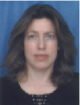
\includegraphics[width=20mm, height=26mm]{edith.png}
\end{minipage}
\end{figure} % Revisado 2017/01/09
\chapter{Antecedentes}
A partir de los estudios realizados por el Grupo de Investigación en Telemedicina de la Universidad Distrital Francisco José de Caldas se han detectado ciertas necesidades y obstáculos para el despliegue de redes de telemedicina. Con base en esto el \textbf{GITEM}, que ha sido pionero en el estudio y desarrollo de soluciones costo efectivas en el área de la telesalud, la teleducación y la administración de los servicios de salud, propone un sistema de información que integra, no solo los aspectos relacionados con la Telemedicina, sino también aquellos que tienen estrecha relación con las tecnologías necesarias para la implementación de los servicios y otros aspectos relevantes.

El proyecto recoge las experiencias que el grupo ha acumulado a través de más de siete años de trabajo continuo en el  área de la telemedicina y las aplica a modelos de gestión de conocimiento para formular una arquitectura conceptual y de software que contribuya a potenciar los ciclos de integración, creación, reproducción y diseminación del conocimiento; a través de un portal especializado.

El \textbf{Sistema de Información para Proyectos de Telemedicina}, conocido desde su primera versión con el nombre genérico de \textbf{SITEM}, es una herramienta de \textit{software libre} orientada a la web, que contiene subsistemas especializados para la gestión de información de diferentes componentes de las redes de telemedicina así como la definición de un modelo que provee los lineamientos para el desarrollo de módulos inéditos. En su más reciente versión explora la integración de \textit{Agentes} notificadores y de Recomendación que analizan constantemente los repositorios de información del sistema para, a partir de un proceso de minería de datos, desplegar información referenciada y adaptada a las necesidades y perfiles de cada uno de los usuarios registrados dentro del sistema. 

Propone un mecanismo para la integración de actores en el área del despliegue de soluciones de Telemedicina proveiendo un escenario ubicuo, basado en tecnologías de la información y un modelo de trabajo colaborativo en red que propende por la construcción evolutiva de una base de información y conocimiento que, asociados a los conceptos de libertad en el uso de la información y el conocimiento, busca elaborar un \textit{recurso público} esencial para el desarrollo de la Telemedicina y la Telesalud en la sociedad.

El modelo conceptual del SITEM aborda a la Telemedicina con un enfoque holístico que trasciende la mera dimensión técnica y tecnológica para abarcar también los aspectos médicos, culturales y de gestión de servicios de salud. Integra, en un solo ambiente, las herramientas básicas de gestión, focalización y orientación de información y conocimiento de diferentes componentes de las redes de Telemedicina que en el estado actual propone reglas formales de estructuración de los almacenes de datos y las bases de conocimiento. La arquitectura del SITEM incluye componentes esenciales para apoyar a los grupos de diseñadores y consultores en la ejecución de sus propuestas en el área que por la complejidad inherente no encuentran un producto que involucre de una forma unificada los diferentes aspectos que requieren ser considerados.

Es común que el desarrollo de soluciones basadas en software Telemédico deban pasar por un proceso de consultoría complejo, y costoso, que muchas entidades de salud son incapaces de costear; de igual manera la concentración de conocimiento en desarrollo de software, el descrédito infundado de soluciones alternativas deliberadamente generalizadas y el desconocimiento por parte de la alta gerencia de nuevas opciones de provisión de productos y servicios hace que todos los proyectos asociados a la Telemedicina y la telesalud parezcan como imposibles de alcanzar sin la inversión de exorbitantes sumas de dinero.
 
\section{Antecedentes del Dominio}
El estudio preliminar de diagnóstico desarrollado por el grupo de investigación GITEM a principios del milenio tenía en mente problemas puntuales para la implementación de servicios médicos prestados a través de medios teleinformáticos en el Distrito Capital\cite{aparicio2000}:

\begin{quote}
“En el momento no existe un diagnóstico real sobre los servicios requeridos en el área de telemedicina, razón suficiente para iniciar un trabajo de campo que establezca la situación actual de servicios médicos y la demanda real, así como la posibilidad de conocer a corto, mediano y largo plazo cuáles serían los costos de inversión que permitirían dar soluciones al problema  de cobertura.

La socialización del conocimiento alrededor de las tecnologías aplicadas al desarrollo de la medicina, es uno de los valores que lleva al éxito de soluciones efectivas en el sector salud, por tal motivo es necesario desarrollar un plan de alfabetización en el sector salud y en el sector gubernamental y académico.

En el país no existen estrategias de investigación en esta área del conocimiento para llevar a cabo un estudio real que permita dar el paso a soluciones verdaderas sobre desarrollo tecnológico o experimental para poder implementar centros de investigación en Telemedicina.

La Universidad Distrital tiene el recurso humano, el conocimiento y la experiencia científica y tecnológica, capaz de dar soluciones tangibles a estas necesidades; unida al conocimiento y experiencia de entidades como clínicas y hospitales  y con la participación de operadores de comunicaciones, puede desarrollar soluciones efectivas a los problemas de salud que afronta la sociedad colombiana.”
\end{quote}

Siendo el estudio totalmente eficaz dio surgimiento al despliegue de nuevos proyectos que aprovecharan de la mejor forma los resultados obtenidos que fueron recopilados en extensos tomos escritos y digitalizados. Para brindar una estructura formal a la documentación, brindar un acceso eficiente de entidades al estudio y gestionar los riesgos asociados al crecimiento de la complejidad a la hora de generar estudios comparativos o de apoyo a la toma de decisiones, se creó al interior del grupo un proyecto de grado denominado \textbf{Sistema de Información en Telemedicina} que en sus primeras fases de desarrollo dio solución parcial al marcar las pautas hacia la integración de información para el \textbf{GITEM} dejando además una investigación valiosa en el tema del desarrollo de software distribuido, interoperable y robusto basado en la filosofía del software libre.

De forma paralela el grupo de investigación implementó, en convenio con \textit{Colciencias}, el Sistema de Referencia y Contrarreferencia para el Distrito Capital, utilizando herramientas de desarrollo propietarias específicamente el middleware .NET de Microsoft con lo que el grupo adquirió experiencia en la desarrollo de aplicaciones siguiendo metodologías efectivas para la construcción de software.

Junto con estos proyectos se desarrolla actualmente cátedra en el área de la Telemedicina ofrecida como seminario inscrito dentro del plan de estudios de la \textit{Maestría en Ciencias de la Información y las Comunicaciones}, lo que ha fomentado el interés investigativo y la formación de profesionales especializados que ha contribuido a la construcción de nuevos saberes en la materia y que se demuestra en la cantidad creciente de proyectos asociados a la línea de investigación.

En la actualidad el grupo de investigación en telemedicina de la Universidad Distrital - \textbf{GITEM}, es catalogado por Colciencias como grupo clase A – el de más alto nivel, y el proyecto SITEM se encuentra institucionalizado por parte del Centro de Investigaciones y Desarrollo Científico con lo que se obtiene una posición de liderazgo en el tema de investigación y se reconoce el trabajo investigativo realizado por el grupo. Todos estos elementos ha generado una base de conocimiento tácito que evidentemente repercute en los sistemas desarrollados, promoviendo y presionando su crecimiento, la adaptación a nuevos requerimientos y el seguimiento de nuevos estándares y legislaciones.

\section{Fases Transcurridas en el SITEM}
En un primer acercamiento el proyecto de investigación se puede asociar a un holotipo proyectivo\cite{hurtado2000} cuyo estadio actual se ha logrado a partir de actividades investigativas que abordan distintos aspectos de la proyección, en la dimensión tecnológica, de los sistemas de Telemedicina. La idea fundamental que siempre ha guiado el proyecto es la de generar un proceso iterativo basado en la construcción y deconstrucción gradual, hermenéutico e incremental de un sistema informático que apoye las labores de consultoría y diseño de redes Telemédicas ahondando de forma asíncrona en cada uno de sus diferentes componentes. 

El proyecto tiene como particularidad tener que cumplir con ambiciosas metas de desarrollo con reducidos recursos técnicos y financieros los cuales deben ser administrados dentro de un ambiente de alta regulación burocrática. El escenario común ha sido el bajo tiempo de permanencia de los integrantes, la ejecución constante de tareas de capacitación, el uso intensivo de tecnologías de la comunicación, el teletrabajo  y la escasa interacción persona a persona. El \textbf{SITEM} inicialmente tenía que ser de calidad, económico y desarrollado rápidamente. Pero teniendo en cuenta lo que \cite{larman2003} nos citaba: “Rápido, barato, bueno: elija dos cualquiera”; con los pies firmemente puestos en el suelo,  dejando a un lado las fuertes esperanzas, debíamos sacrificar un aspecto y el único que se disponía era la rapidez en que versiones estables del proyecto habrían de ver la luz - los conceptos fundamentales de desarrollo de aplicaciones de software libre aportarían varias claves para minimizar el impacto de este sacrificio.

\begin{figure}
 \centering
 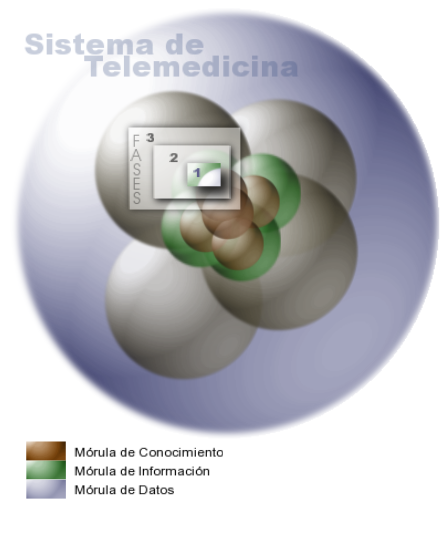
\includegraphics[width=156mm, height=195mm]{modelo_fases.png}
 \caption{Aproximación incremental a un sistema de Gestión de Conocimiento}
 \label{modelo1}
\end{figure}

Con esto como patrón fundamental el grupo de desarrollo plantea un modelo general en donde los objetivos de producir datos, consumir información y compartir conocimiento en el área de interés será alcanzado en varias fases\footnote{A través del presente documento se utilizan los términos de fase en el proceso investigativo y fases del Proceso de Desarrollo del Sistema Software. Las dos se suponen diferentes y su interpretación e importancia están asociados al contexto en el que se ubican.} de las cuales se describen los alcances de aquellas que han culminado.

La figura \ref{modelo1} muestra el proceso de estructuración de un sistema de telemedicina como una sucesión de fases que generan las dimensiones de datos, información y conocimiento de un grupo de componentes dado. El sistema visto como un \textit{holos} presenta al investigador una gran cantidad de datos que en la medida que se descubren, recolectan, observan y registran se van convirtiendo en información susceptible de ser descrita, analizada, integrada y comparada acercándose cada vez más a un conocimiento refinado. El carácter de discernible - el momento en que las dimensiones se solapan en grado sumo, se evidencia con el aumento colectivo de especialización en la materia y en nuestro caso, con el grado de inmersión de los usuarios en el SITEM.

En el transcurso de las fases solo se manejan ciertos aspectos que incremental y constructivamente se suman para crear un modelo cada vez más exacto del sistema con base en las diferentes \textit{mórulas} de datos, información y conocimiento generadas. Aunque en el gráfico se muestra un tanto discretos y exactos, los límites existentes entre las tres mórulas principales - datos, información, conocimiento; son en la realidad difusos. Esto dificulta la consecución del objetivo de cada fase que es tratar de profundizar en uno o varios componentes del holos - conseguir especificidad en el modelo.

Si se consideran los aspectos meramente técnicos del SITEM se corre el riesgo inminente de diseminación en regiones poco profundas del sistema - dispersión en la mórula de datos - razón por la cual la herramienta software se ha convertido en un artefacto intermedio y no en el fin último de la investigación.

\subsection{Sistema de Información para Telemedicina – Fase I}
Con la primera fase de desarrollo del SITEM se logró un conocimiento amplio de los componentes de las redes de telemedicina y sus interrelaciones basado en una investigación exploratoria y descriptiva realizada por los integrantes del grupo GITEM. 

También se determinaron las características esenciales de diferentes portales que implementaban en cierto grado la funcionalidad esperada para el SITEM vislumbrando con este estudio la necesidad de crear un producto software adaptado a las necesidades del entorno distrital, teniendo en cuenta que ninguno de los portales analizados brindaba acceso a información pertinente, confiable, actualizada y estructurada en torno a las redes de telemedicina en idioma español.

La cuestión fundamental que se resolvió en esta fase fue la definición de un modelo para la estructuración y administración de información relevante para los participantes en el diseño, análisis y desarrollo de las redes de Telemedicina. Además se definió un modelo de negocios que lograba mostrar las interrelaciones que tendría el sistema con los proyectos del grupo y un conjunto representativo de portales relacionados temáticamente; encontrando un costo de oportunidad adecuado. En la actualidad dicho modelo de negocios cobra mayor vigencia con la tendencia generalizada de desmonte de inversión en los portales más importantes a nivel mundial – siendo quizás \textbf{ipath}, también basado en la filosofía del software libre, uno de los únicos que continúan activos y en crecimiento, demostrando de paso que el esquema propuesto - gestionado eficientemente, es adecuado para el desarrollo y mantenimiento de sistemas de esta clase.

Al momento de desarrolló de esta fase el grupo de investigación no contaba ni siquiera con un portal web por lo que la arquitectura propuesta incluyó al portal del grupo como un subsistema del SITEM compartiendo de esta forma tanto la plataforma tecnológica como el modelo conceptual, lo que difuminó un poco los alcances reales del Sistema y su implementación no pasó de ser un prototipo de baja funcionalidad. 

Los alcances y logros efectivos de esta fase fueron:

\begin{itemize}
\item Descripción del Modelo de Negocio.
\item Propuesta de Desarrollo
\item Creación de la Arquitectura general del Sistema.
\item Desarrollo del sitio web del grupo GITEM e integración conceptual del SITEM dentro de los proyectos del grupo.
\item Elaboración de los Modelos básicos de Requisitos, análisis y diseño.
\item Estudios sobre filosofía de Software Libre.
\item Construcción de un Prototipo de baja funcionalidad conocido como SITEM versión 0.1, bautizada internamente como \textbf{Kauil}.
\end{itemize}


\begin{figure}
 \centering
 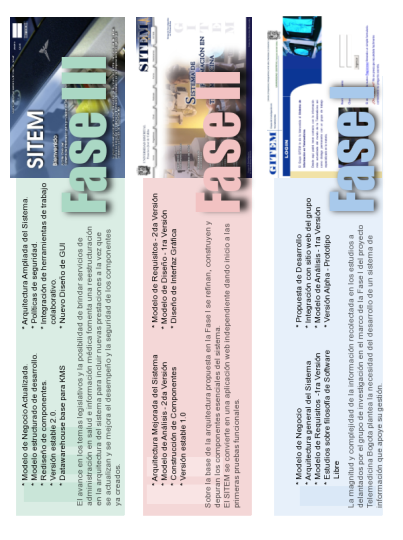
\includegraphics[width=142mm, height=190mm]{fase_sitem.png}
 \caption{Fases transcurridas en el desarrollo del SITEM}
 \label{fase_sitem}
\end{figure}

\subsection{Sistema de Información para Telemedicina – Fase II}

Los modelos de requisitos, análisis y diseño de la primera fase sirven de base para proponer arquitectura general para el Sistema de Información para Proyectos de Telemedicina y con el inicio de la segunda fase se emprenden las actividades necesarias para la construcción de los componentes de software que concretaban dicha arquitectura. Para poder minimizar los riesgos asociados al proyecto se adaptó el \textit{Proceso Unificado de Desarrollo de Software} a las especificidades de desarrollo del Sistema, lo que favoreció efectivamente su elaboración, implementación, mantenimiento y crecimiento.

La arquitectura general se vio poco afectada pero cada uno de los subsistemas componentes fueron más finadamente caracterizados resultando en un modelo de análisis y diseño mejor definido que integraba elementos no tratados en la fase inicial. Debido a la naturaleza del SITEM, el grupo de investigación decide separar los hilos de desarrollo del Sistema y del proceso de estructuración del sitio web del grupo. El SITEM por primera vez se puede acceder desde \textit{Internet} gracias al despliegue que se realiza sobre la plataforma de hardware y software brindada por la \textit{Universidad Distrital}. 

En esta fase se realiza el modelado de datos y se esbozan las primeras rutinas de manejo se seguridad. Para la construcción de componentes se utilizan herramientas de software libre y el grupo de desarrollo aumenta a cinco integrantes. El trabajo se encuentra, con excepción del director del proyecto, soportado y ejecutado por estudiantes de pregrado del proyecto curricular de Ingeniería Electrónica convirtiéndose en el \textbf{primer proyecto de desarrollo de software libre realizado por el GITEM} e involucra la formación transdisciplinar de un grupo de sus integrantes.

Los alcances de esta fase fueron:
\begin{itemize}
\item Arquitectura Mejorada del Sistema
\item Modelo depurado de Requisitos
\item Modelo de Análisis - Segunda Versión
\item Modelo de Diseño
\item Construcción de Componentes software soportado en su totalidad por herramientas de software libre.
\item Diseño de Interfaz Gráfica
\item Versión estable 1.0 y bautizada internamente como \textbf{Gucumatz}.
\item Adaptación del Proceso Unificado de Desarrollo de Software a las especificidades del SITEM.
\item Configuración de la plataforma tecnológica de despliegue del sistema.                                            \end{itemize}

Al final de la fase se obtiene un aplicativo que presenta avances en todos los subsistemas propuestos.


\subsection{Sistema de Información para Telemedicina – Fase III}

El almacén de datos obtenido en la segunda fase aunque interesante es poco funcional cuando se trata de aplicar directamente al apoyo de la implementación de soluciones basadas en software telemédico. Estos proyectos presentan retos adicionales en la medida que deben pasar por procesos de consultoría complejos y costosos que muchas entidades de salud públicas son incapaces de costear. Otros riesgos están asociados a la desinformación que injustificada y deliberadamente mantiene la empresa privada en cuanto a que con software libre no se siguen buenas prácticas de desarrollo de software, ni se obtienen sistemas seguros que garanticen la integridad de los datos - conceptos totalmente alejados de la realidad que pueden minar el juicio objetivo de administradores médicos no especializados en telemedicina - y mucho menos en teleinformática, en cuanto a la posibilidad de alcanzar sistemas eficientes y eficaces sin la inversión de exorbitantes sumas de dinero. 

Es común encontrar en el ámbito colombiano casos de éxito de aplicaciones telemédicas en entidades de salud privadas pero son escasas las aplicaciones en entidades públicas de segundo o tercer nivel. Evidentemente el uso, promoción y difusión de software libre es una práctica necesaria para poder implementar aplicaciones con altos niveles de calidad que beneficien al grueso de la población.

SITEM en esta fase genera una herramienta que ordena la información lógicamente y permite su acceso personalizado en áreas del conocimiento que tienen inferencia sobre las redes de telemedicina: medicina básica, tecnologías de interconexión, equipos de telemedicina, instituciones de salud, entidades prestadores de servicios de telecomunicaciones, entre otras; así mismo integra una serie de servicios en línea que propenden por la consolidación de una comunidad en Telemedicina basada en Internet, figura \ref{sitem_faseIII} .

Se consolida un proceso de desarrollo de software adaptado a las especificidades del grupo de investigación el cual trata de extraer lineamientos de las prácticas mundialmente aceptadas de procesos y métodos como son el Proceso Unificado, Métrica 5, Normas de Calidad ISO 9000 y EFQM. Se trata de buscar el aseguramiento de la calidad en el desarrollo, la interoperabilidad, escalabilidad y el uso extensivo de software libre. Se documenta todas las etapas involucradas en la creación de la aplicación para que sirva de plantilla a sistemas relacionados y se formaliza las áreas de capacitación a partir de ciclos genéricos de transferencia de conocimiento apoyados en tecnologías de la información.

\begin{figure}
 \centering
 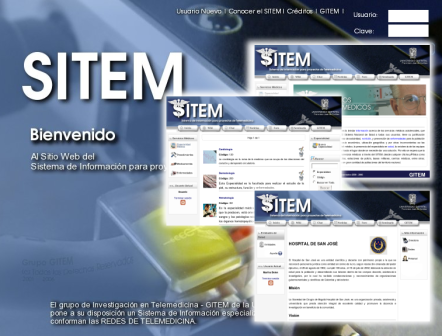
\includegraphics[width=156mm, height=118mm]{pagina_principal.png}
 \caption{Sistema de Información para proyectos de Telemedicina. Interfaz de Usuario en la Fase III}
 \label{sitem_faseIII}
\end{figure} 	% Revisado 2017/01/09
\chapter{Contexto Teórico}

A consideración del grupo, dos aspectos del proyecto son innovadores en el ámbito colombiano: el modelo de dominio e información del contexto de la proyección y diseño de soluciones en Telesalud; y el modelo de federación de aplicaciones que permiten el despliegue de soluciones de alta funcionalidad a bajo coste explotando - y colaborando con, el movimiento de Software Libre y Código Abierto (FLOSS).

El presente capítulo provee la base teórica que sustenta los modelos, presentando las estructuras de información y sus relaciones, abordando el marco legislativo y demás temáticas que son necesarias para caracterizar los componentes primordiales de los Sistemas. Teniendo en cuenta el carácter evolutivo del proyecto software y como referencia para posteriores desarrollos soportados en el SITEM, también se tratan cuestiones relevantes del proceso de ingeniería que guió la integración del sistema.

\section{eSalud}
Teniendo en consideración que el servicio de más alto nivel de la red es la eSalud, es necesario abordar su concepto con el fin de tener un marco para la comprensión del modelo de dominio que se presentará en un capítulo posterior.

La eSalud es definida por la organización Mundial de la Salud (OMS) \cite{oms2016} como \begin{quote}el apoyo que la utilización costo eficaz y segura de las tecnologías de la información y las comunicaciones ofrece a la salud y a los ámbitos relacionados con ella, con inclusión de los servicios de atención de salud, la vigilancia y la documentación sanitarias, así como la educación, los conocimientos y las investigaciones en materia de salud\end{quote}, en si es un término que define un campo multidisciplinar que integra componentes de diferentes áreas del saber que incluye entre otros a la medicina, la ingeniería electrónica, la telemática, la informática, la ingeniería de sistemas, la inteligencia artificial, la biónica, la psicología, la sociología, la antropología, las geociencias, entre muchas otras. Las redes eSalud consideran elementos que van mucho más alla del simple despliegue de redes tecnológicas de intercomunicación y se plantean como redes de interacción social cuyo objetivo primario - más no el único, es la prestación de servicios médicos y relacionados.

Dependiendo el grado en que se presente cada uno de los elementos mostrados en la figura ~\ref{elementosred} y de la mayor o menor correlación entre ellos, se pueden crear sistemas de eSalud que se acerquen al ideal de proveer servicios de salud de alta calidad. 

La OMS y la Unión Internacional de Telecomunicaciones (ITU) proveen \cite{ituoms2012} un método que podría ser utilizado para abordar el desarrollo de proyectos de eSalud complejos, dinámicos y evolutivos. 

\begin{figure}
 \centering
 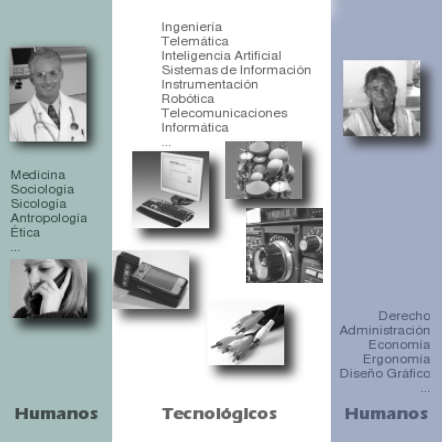
\includegraphics[width=130mm]{sistema_telemedicina.png}
 \caption{Modelo simple de categorías para nodos de una red de eSalud.}
 \label{elementosred}
\end{figure}

\subsection{Componentes Principales de eSalud}

La eSalud comprende áreas que no tienen una división concreta pero se enfocan en ciertos aspectos de interés:

\begin{itemize}
 \item Telemedicina: Provisión remota de servicio clínicos
 \item Telesalud: Telemedicina, complementada con la prestación remota de otros servicios tales como entrenamiento médico, monitoreo de pacientes, cuidado médico, gestión administrativa, etc. 
 \item mSalud: telesalud con el apoyo de dispositivos móviles.
 \item Registro Médico electrónico: Conocido como Historia Clínica Electrónica. Comprende los mecanismos que permiten registrar en un entorno digital seguro, la información sobre los eventos de salud de cada paciente.
 \item eAprendizaje/eEnseñanza: Servicios de enseñanza/aprendizaje de ciencias médica y afines, en modalidad a distancia o virtual.
\end{itemize}

Cabe la pena aclarar que la pluralidad de componentes no es más que un esfuerzo para abordar en un único modelo, todas las tendencias que se han presentado en la evolución de la eSalud. En alguna literatura los términos son intercambiables dependiendo el enfoque del autor. \cite{oms2010}.
\section{Marco Legislativo y Normativo}

OpenSITEM es un sistema que gestiona información sobre diferentes áreas del saber de acuerdo a las categorías de los nodos que se definan. Cada aspecto (atributos, interfaces, interoperaciones) está en un marco legislativo y normativo concreto, o está asociado a estándares y normas de uso extendido o de facto aceptadas en el mundo. La información de OpenSITEM que sea de acceso público no podrá incluir protección por derechos de autor que restrinjan su difusión \cite{congreso565},\cite{congreso23}. Debido a esto, el código fuente de OpenSITEM es cubierto por una licencia abierta que se ciñe a la normatividad expresada en la Ley 565 de 2000: adopción del Tratado de la OMPI sobre Derechos de Autor y complementarias para garantizar que todos los aspectos tanto técnicos como conceptuales estén debidamente registrados \cite{congreso565},\cite{congreso44},\cite{congreso1360}. 

OpenSITEM es una plataforma para la definición de nodos y no es posible \textit{a priori} definir el marco legislativo que regirá cada nodo o categoría. Sin embargo, se describe a continuación un marco relacionado con las categorías base que se han definido en el primer modelo del sistema.

\subsection{En el Ámbito de los Servicios Médicos}

El Derecho a la Salud ha sido reconocido por normas y pactos internacionales contenidos en tratados sobre Derechos Humanos, Económicos, Sociales, y Culturales  (DHESC). Esos acuerdos han sido ratificados por Colombia para su cumplimiento como un derecho de los ciudadanos. “La Corte Constitucional; ha señalado que el inciso segundo del artículo 93 de la Carta Política confiere rango constitucional a todos los tratados de derechos humanos, económicos,  sociales y culturales, ratificados por Colombia y referidos a derechos que ya aparecen en la Carta” \cite{sentencia1319} como ocurre con el Derecho a la Salud. 

Al Ministerio de Salud y Protección Social, le corresponde expedir las normas técnicas y administrativas de obligatorio cumplimiento para las Entidades Promotoras de Salud del régimen contributivo, las Instituciones Prestadoras de Salud del Sistema General de Seguridad Social en Salud, las Administradoras del Régimen Subsidiado y para las Direcciones Seccionales, Distritales y Locales de Salud en cuanto al objetivo de cumplimiento en el desarrollo de actividades de protección específica, detección temprana y atención de enfermedades de interés en Salud Pública. 

A continuación se registra la normatividad que se tuvo en cuenta al momento de definir los componentes actuales del subsistema de servicios médicos en cuanto a la relevancia que se tiene tanto para la proyección de nuevas redes de eSalud, como para apoyar los sistemas básicos ya existentes. Es de anotar que lo contemplado en las leyes nacionales es, en su mayoría, derivado de normas internacionales que han sido objeto de detallados estudios y reconocidas técnicamente con base en las experiencias vividas por los profesionales de esta área. 

\begin{description}

\item[Ley 1751 de 2015]. Por medio de la cual se regula el derecho fundamental a la salud. Es una ley estatutaria que surge a partir de la debacle del proceso de reforma y tiene como efecto positivo el elevar a la salud como un derecho fundamental. Entró en rigor a partir del año 2017 y da lineamientos para reestructurar el sistema de salud a partir del desarrollo de \textit{redes de servicios} públicos, privados o mixtos. También declara la necesidad de establecer políticas relacionadas con la salud tales como la política para la información, la política de innovación, ciencia y tecnología; y la política farmacéutica nacional.

\item[Ley 1419 de 2010].  Por la cual se establecen los lineamientos para el desarrollo de la telesalud en Colombia. Define las redes de telesalud y el aprendizaje en telesalud como ejes principales de la gestión del conocimiento en salud. Si bien esta ley obliga a desarrollar el mapa de conectividad, aún en el 2017 no se encuentra uno que esté disponible para los ciudadanos.

\item[Resolución 2182 de julio 9 de 2004] Con esta resolución se definían las Condiciones de Habilitación para las instituciones que prestan servicios de salud bajo la modalidad de Telemedicina. Fue derogada por el artículo 11 de la \textbf{resolución 1043 de 2006}, con la cual se establecen las condiciones que deben cumplir los Prestadores de Servicios de Salud para habilitar sus servicios e implementar el componente de auditoría para el mejoramiento de la calidad de la atención y se dictan otras disposiciones. 

Posteriormente, con la \textbf{Resolución 1448 de 8 de Mayo de 2006} se regula la prestación de servicios de salud bajo la modalidad de telemedicina y establece las condiciones de habilitación de obligatorio cumplimiento para las instituciones que prestan servicios de salud. Esta resolución aclara que las actuaciones de los médicos en el ejercicio de la prestación de servicios bajo la modalidad de telemedicina se sujetarán a las disposiciones establecidas en la \textbf{Ley 23 de 1981} y demás normas que la reglamenten, modifiquen, adicionen o sustituyan.

\item[Resolución 4678 de noviembre 11 de 2015] Con esta resolución, modificada por la Resolución 1113 de 2017, el Ministerio de Salud y Protección Social adopta una Clasificación Única de Procedimientos en Salud (CUPS) la cual "...corresponde a un ordenamiento lógico y detallado de los procedimientos y servicios en salud que se realizan en al país, en cumplimiento de los principios de interoperabilidad y estandarización de datos utilizando, para tal efecto, la identificación por un código y una descripción validada por los expertos del país."\cite{minsalud4678}. La Clasificación Única de Procedimientos en Salud adaptación para Colombia, se implementa por \textbf{Resolución 365 de 1999}. Su primera publicación se presenta en un solo volumen que contiene la Lista Tabular y el Índice Alfabético. A partir de dicha resolución se realizó la primera actualización de la CUPS (1°A-CUPS) mediante la \textbf{Resolución 2333 de 2000}. En el año 2016, mediante la Resolución 3804, se establece el procedimiento para la actualización de la CUPS, con lo que el Ministerio espera darle una mayor agilidad al proceso.

\item[Resolución 1830 de junio 23 de 1999] adopta para Colombia, “Las codificaciones únicas de especialidades en salud, ocupaciones, actividades económicas y medicamentos esenciales" para el Sistema Integral de Información del SGSSS - SIIS 

\item[Resolución 1895 de noviembre 19 de 2001] por la cual se adopta para la codificación de morbilidad en Colombia, La Clasificación Estadística Internacional de Enfermedades y Problemas Relacionados con la Salud - Décima revisión. 

\begin{quote}
Considerando que en la 43a. Asamblea Mundial de la Salud llevada a cabo en 1990, fue aprobada por la Conferencia Internacional la Clasificación Estadística Internacional de Enfermedades y Problemas Relacionados con la Salud - Décima revisión -, (CIE-10) en la cual Colombia no expresó objeciones y adquirió el compromiso de implementarla. Resuelve Adoptar para la codificación de morbilidad en Colombia, la Clasificación Estadística Internacional de Enfermedades y Problemas Relacionados con la Salud -Décima revisión-, contenida en la publicación científica No.554 de la Organización Panamericana de la Salud, presentada en tres volúmenes: V1. Lista de Categorías; V2 Manual de Instrucciones; V3 Índice Alfabético.\end{quote} 

\item[Resolución 1995 de julio 8 de 1999] por la cual se establecen normas para el manejo de la Historia Clínica.

La Historia Clínica es un documento de vital importancia para la prestación de los servicios de atención en salud y para el desarrollo científico y cultural del sector, \textit{es un documento privado, obligatorio y sometido a reserva}, en el cual se registran cronológicamente las condiciones de salud del paciente, los actos médicos y los demás procedimientos ejecutados por el equipo de salud que interviene en su atención. Dicho documento únicamente puede ser conocido por terceros previa autorización del paciente o en los casos previstos por la ley. 


\item[Circular 015 de abril 4 de 2002] estándar de historias clínicas y registros, establece la obligatoriedad de definir procedimientos para utilizar una historia única institucional. Ello implica que la institución cuente con un mecanismo para unificar la información de cada paciente y su disponibilidad para el equipo de salud. No es restrictivo en cuanto al uso de medio magnético para su archivo, y sí es expreso en que debe garantizarse la confidencialidad y el carácter permanente de registrar en ella y en otros registros asistenciales.


\item [Decreto 2092 de 2 de Julio de 1986], Por el cual se reglamenta parcialmente los Títulos VI y XI de la \textbf{Ley 09 de 1979}, en cuanto a la elaboración, envase o empaque, almacenamiento, transporte y expendio de Medicamentos, Cosméticos y Similares. Se dan las Disposiciones Generales y Definiciones, el Registro Sanitario de Medicamentos, Cosméticos y Similares.
\end{description}

\subsection{En el Ámbito del Desarrollo de Redes Teleinformáticas}

\begin{description}
\item[Documento CONPES 3072] Aunque no es una norma regulatoria, es una declaración oficial del gobierno colombiano acerca de la necesidad de fomentar las Tecnologías de la Información para potenciar la absorción, creación y divulgación del conocimiento por medio del desarrollo sostenible en las infraestructuras física, de información y social. Según \cite{mincomunicaciones3072}:  “... para que el país pueda ofrecer un entorno económico atractivo y participar en la economía del Conocimiento, resulta indispensable desarrollar una sociedad en la que se fomente el uso y aplicación de las Tecnologías de la Información. A través de estas Tecnologías, se puede efectuar un salto en el desarrollo en un tiempo relativamente breve, mucho menor del que se necesita para superar el déficit de infraestructura física.".

El documento CONPES brinda un referente válido pues la mayoría de los objetivos estratégicos del OpenSITEM contienen el espíritu expresado en diferentes partes del mismo.

\item[Documento CONPES 3582] Política Nacional de Ciencia, Tecnología e Innovación. En el cual se enfatiza el desarrollo de la salud y la tecnología como mecanismos de generación de valor social.

\item[Resolución 087 de 1997] “Por medio de la cual se regula en forma integral los servicios de Telefonía Pública Básica Conmutada (TPBC) en Colombia.” En donde claramente se expresa que: \begin{quote}
Los servicios de TPBC deberán ser utilizados como instrumento para impulsar el desarrollo político, económico y social del país con el objeto de elevar el nivel y la calidad de vida de los habitantes en Colombia. Los servicios de TPBC serán utilizados de manera responsable para contribuir a la defensa de la democracia, a la promoción de la participación de los colombianos en la vida de la Nación y la garantía de la dignidad humana y de otros derechos fundamentales consagrados en la Constitución Política, y para asegurar la convivencia pacífica.\end{quote} 

Esta resolución presenta particular importancia para la extracción de elementos semánticos y algunos componentes necesarios en las redes de telecomunicaciones basadas en telefonía conmutada. Algunas heurísticas usadas en el subsistema de consultoría también se basan en apartes de esta resolución.

\item [Manual de Calidad de Servicio] “Con este Manual de calidad de servicio (QoS) se especifican los parámetros de calidad de servicio de red que permiten el suministro de servicios a los clientes y los usuarios, satisfaciendo sus expectativas de calidad de servicio. Estos parámetros tienen que ver tanto con la implementación del servicio como con su utilización continua. Asimismo, la calidad de servicio se relaciona con todos los aspectos relativos a la evaluación y gestión de las redes.”\cite{ITU2004}

Sus principales aspectos son recogidos en \cite{crtcondiciones} y \cite{crtindicadores}  las cuales sirven de base para el proyecto de resolución\cite{crtqos} de la Comisión de Regulación de Comunicaciones y que especifica entre otros: las definiciones relativas a la QoS, parámetros de medición, variables y propiedades técnicas de diferentes enlaces. Aunque el objetivo principal de este manual es el de garantizar la QoS en un sistema de telecomunicaciones dado es importante notar que sus indicaciones deben ser tenidas en cuenta al momento de proyectar los servicios de telecomunicaciones en un sistema de telemedicina dado. En estos aspectos también se considera dentro del modelado de ciertos componentes del OpenSITEM las recomendaciones de la UIT en \cite{ITUG1000} y \cite{ITUG1010}, las cuales aún no tienen un equivalente en la normatividad colombiana pero son de uso extendido alrededor del orbe.

\end{description}

\subsection{En el ámbito del Tratamiento de Datos e Información}  

\begin{description}
 \item[Ley 1581 de 2014 y Ley 1266 de 2008]. Estas leyes están relacionadas con la protección de los datos personales y el aseguramiento de la privacidad de la información personal.
 
\end{description}
\section{Aspectos Claves en la Gestión y Dirección del Conocimiento}

Como se aclaró anteriormente, OpenSITEM es una federación de diferentes tipos de sistemas software y sirve de soporte para el trabajo de los equipos de diseño de redes de eSalud del grupo de investigación GITEM (o similares). En esa línea, parte de su funcionalidad está enfocada en brindar apoyo a los flujos de trabajo de comunidades de práctica yu por tanto es necesario que se aborden aspectos relacionados con la gestión del conocimiento. A continuación se presenta la aproximación conceptual de está área.

\subsection{Acerca del conocimiento}

En la presente investigación conocimiento es entendido como un concepto que encierra, entre otras, las siguientes definiciones y se usarán de acuerdo a su contexto como partes complementarias de una misma meta – definición.

De acuerdo con Gunter Dueck\cite{dueck2001}, el conocimiento es un concepto que puede tener componentes en una o varias de las siguientes dimensiones:

\begin{itemize}
\item  \textbf{Episteme} -\textit{ Dimensión abstracta – o metafísica}, en forma de generalizaciones, bases, leyes y principios científicos.

\item \textbf{Phronesis }– \textit{Dimensión práctica}, relativa al conocimiento pragmático discernido a través de las practicas aceptadas por la sociedad.

\item \textbf{Techne} – \textit{Dimensión técnica}, relativa a la forma de hacer las cosas, de la realización de actividades concretada en la forma de manuales, procedimientos y comunidades de práctica.

\item \textbf{Metis} – \textit{Dimensión objetiva}, como forma de volver corpóreo, real y sustancial la conjugación de los otros tipos de conocimiento.
\end{itemize}

Esta concepción multidimensional extiende y explica la taxonomía del conocimiento dada por los griegos:

“El conocimiento incluye restricciones implícitas y explícitas entre objetos (entidades), operaciones y relaciones, que permiten recoger heurísticas generales y específicas así como los procedimientos de inferencias relacionados con la situación a modelar”.\cite{sowa1984}

Otros autores despojan del sentido filosófico y colocan su definición en un plano simple y utilitario: “El conocimiento es información organizada y analizada para hacerla comprensible y aplicable a la resolución de problemas y toma de decisiones”.\cite{turban1992}. Si bien esta es una definición reduccionista, sirve de base para las propuestas de representación de conocimiento en documentos XML - comúnmente denominadas \textit{ontologías}. 


\subsection{Ciclo de Conocimiento}

Múltiples factores deben ser considerados cuando se trata de capturar, crear y diseminar el conocimiento dentro de un grupo de personas. La no homogeneidad en los medios de almacenamiento de conocimiento es uno de ellos. El conocimiento - en cualquiera de sus formas, puede estar guardado en diferentes partes que van desde entidades biológicas - mente humana, genes; a repositorios de conocimiento estructurado tales como ontologías, grafos de relación o mapas mentales.

Otro factor importante es la capacidad de acceso al conocimiento que es muy diferente al mero hecho de acceder a una fuente de conocimiento dada. En \cite{nokata1995} se considera que el conocimiento puede estar en dos estadios con propiedades diferentes: tácito y explícito. 

\begin{itemize}
\item \textbf{Conocimiento tácito:} Este conocimiento se corresponde con el conocimiento obtenido a través de la experiencia, conocimiento simultáneo  y conocimiento análogo. Esta forma de conocimiento usualmente se encuentra en medios de almacenamiento biológicos como la mente humana.

\item \textbf{Conocimiento explícito:} Se corresponde con el conocimiento racional, conocimiento secuencial, y conocimiento digital y se encuentra almacenado en documentos, bases de conocimiento, ontologías o cualquier otro medio abstracto de representación.
\end{itemize}

En \cite{liebowitz1998} se establece un tercer estadio llamado conocimiento implícito.

\begin{itemize}
\item \textit{Conocimiento Implícito:} Acceso directo mediante consulta y discusión. Requiere la localización y comunicación previa de conocimiento informal.
\end{itemize}

Un \textit{Ciclo de Conocimiento} es el proceso por el cual el conocimiento se transforma de tácito a explícito y viceversa por medio de las siguientes actividades:

\begin{itemize}
\item \textbf{Socialización:} Compartir conocimiento tácito entre individuos. El conocimiento permanece siendo tácito sin ser transformado en explícito. Este tipo de patrón no es muy interesante debido a su naturaleza tácita (Tácito - Tácito).

\item \textbf{Articulación:} Alguien transforma el conocimiento tácito en explícito (Tácito - Explícito).

\item \textbf{Síntesis:} Combinación de conocimiento explícito para crear nuevo conocimiento explícito  (Explícito - Explícito).
 
\item \textbf{Interiorización:} Proceso de transformar conocimiento explícito en tácito (Explícito - Tácito).
\end{itemize}

\begin{figure}
 \centering
 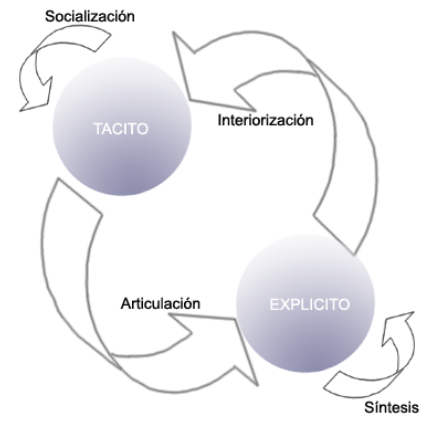
\includegraphics[width=100mm]{Ciclo_Conocimiento.png}
 \caption{Ciclo de Conocimiento}
 \label{ciclo_conocimiento}
\end{figure}

El flujo de conocimiento organizacional más importante es la transformación del conocimiento tácito en explícito \cite{davies2011}, esto es, la \textit{articulación} que se apoya en procesos avanzados de socialización. Esto permite acumular conocimiento explícito que puede ser compartido y accedido por los miembros de la organización. Por el contrario, la interiorización es el proceso natural llevado a cabo a través del aprendizaje individual por parte de los integrantes de la organización, esto es, la asimilación de conocimiento. 

El tercer flujo de conocimiento relacionado con la transformación de conocimiento es la \textit{combinación} o síntesis. En este caso se transfiere conocimiento a otra forma explícita de conocimiento. Un ejemplo sería el cambiar el formato de una base de conocimiento, agrupar ontologías o refinar heurísticas. Este tipo de flujo de conocimiento es importante para seleccionar, combinar y distribuir el conocimiento existente con diferentes fines. Por ser quizás el flujo de conocimiento más formal en OpenSITEM algunos componentes específicos implementan flujos de síntesis de conocimiento.

El cuarto flujo del ciclo de vida del conocimiento permite transformar conocimiento tácito en otras formas de conocimiento tácito mediante procesos de socialización. Un ejemplo de esto es cuando se transfiere conocimiento tácito de un experto a un ingeniero de conocimiento en una entrevista personal.

\subsection{Tecnologías del Conocimiento}

En la actualidad el conocimiento se considera un activo fundamental y como lo expresa \cite{gang2007}, tiene dos propiedades de vital importancia para contribuir al desarrollo de las organizaciones o comunidades de práctica:

\begin{itemize}
\item \textbf{Es explicable.} Cuando no se evidencia esta propiedad el conocimiento permanece tácito y en ninguna medida puede considerarse como perteneciente a la comunidad o la organización. Es entonces una tésis que solo aquel conocimiento que se ha convertido en explícito es el que posee una organización; de otra manera es propiedad exclusiva del individuo.

\item \textbf{Se puede comunicar y compartir.} Cuando no se toman medidas que formalicen estas actividades el conocimiento se pierde. Es decir, la organización o comunidad debe tener procesos conocidos que garanticen flujos de conocimiento basados en la síntesis, interiorización y socialización.
\end{itemize}

En general para que el conocimiento pueda generar ventajas competitivas debe ser gestionado de alguna manera. Esta necesidad dio surgimiento a dos áreas de investigacion comunmente agrupadas bajo el concepto de Tecnologías de Conocimento: Ingeniería de Conocimiento y Gestión de Conocimiento. 

Uno de los primeros problemas que deben atacar las tecnologías de conocimiento es el asociado con el Modelado de Conocimiento. En \cite{benafia2016} se expresan algunos principios a tener en cuenta cuando se modela el conocimiento:

\begin{itemize}
\item \textbf{Definición de roles de conocimiento}. El conocimiento se puede dividir en unidades atómicas que tienen propiedades irreductibles y que se asocian para lograr funciones que identifican dicha unidad.

\item \textbf{Identificación de tipos de conocimiento.} Cada unidad de conocimiento debe enmarcarse en uno o varios de los siguientes tipos de conocimiento: de tareas, inferencial, del dominio, ontologías del dominio, modelos del dominio. 

\item \textbf{Capacidad de ser compartido y reutilizado.} Las unidades de conocimiento pueden ser expresadas usando lenguajes y reglas formales. Lo que permite que pueda ser entendido por entidades con roles de conocimiento definidos.

\item \textbf{Uso de modelos gráficos.} La unidades de conocimiento pueden ser representadas mediante grafos tipo red en los cuales tanto los nodos como las rutas de interconexión son unidades atómicas de conocimiento.
\end{itemize}


\subsection{Gestión de conocimiento}

La gestión del conocimiento es de esos conceptos \textit{polisémicos} que no pocos autores pretenden consolidar en una sola definición \cite{girard2015}. En este proyecto partimos de una visión sistémica que lo transcienda a lo que en investigación holística se comprende como sintagma\cite{hurtado2000}. La \textit{gestión de conocimiento}, como se percibe en la presente investigación, es “una unión sintagmática de diversos paradigmas” \cite{hurtado2000}. Fue \textit{Karl Wiig}, quien usó el término de \textit{gestión de conocimiento} por primera vez durante una conferencia en Suiza y a partir de ese momento diversos autores han conceptualizado el término surgiendo definiciones parciales tales como:

“La Gestión de Conocimiento es la construcción y aplicación sistemática, explícita y deliberada de conocimiento para maximizar la efectividad organizacional con respecto al conocimiento, por lo que usa sus activos de conocimiento”\cite{wiig1993}

“La Gestión de Conocimiento es el proceso de capturar experiencia colectiva organizacional donde ésta resida (por ejemplo, bases de datos, documentos, mentes humanas) y su distribución allá donde pueda ayudar a mejorar los resultados”\cite{hibbard1997}

“La Gestión de Conocimiento es la gestión y control explícito del conocimiento en una organización para lograr los objetivos de la organización” (van der Spek and Spijkervet, 1997)

Consecuente con la concepción de la gestión de conocimiento como un sintagma se puede concebir un paradigma asociado a un proceso con ciertas actividades implicadas: 

\begin{itemize}
\item Identificación y mapeo de bienes intelectuales de la organización.
\item Generación de conocimiento nuevo que permita obtener una ventaja competitiva. 
\item Recopilación accesible de información organizacional. 
\item Compartir buenas prácticas y tecnología, incluyendo técnicas de trabajo en grupo.
\end{itemize}

Este paradigma explora el conocimiento técnico, pragmático y objetivo considerando que la conjugación de leyes rígida e epistemológicas van en contravía de la dinámica misma de los sistemas. La articulación de este conocimiento debe ser mantenido de alguna forma en la organización, y de ahí surge el concepto de Memoria Corporativa. El saber hacer está completamente diseminado en la organización y debe ser integrado de forma coherente para facilitar el acceso al mismo y su reutilización, esto es, expresarlo en forma de memoria corporativa. 

Las memorias corporativas se consideran un elemento clave para gestionar el conocimiento porque facilitan su conservación, distribución y reutilización. Van Heijst define la memoria corporativa como una “representación de conocimiento e información organizacional explícita y persistente”, mientras que en (Nagenda y Plaza, 1996) se define como “los recursos colectivos de datos y conocimiento de una compañía, incluyendo experiencias en proyectos, experiencia en resolución de problemas, etc”. En (Abecker, 1998), una memoria corporativa es referida como “un contenedor que integra información contextual, documentos e información no estructurada, que facilita su uso y reutilización”.

%\section {Ontologias}


1.5 ONTOLOGÍAS

Tal como ocurre con el conocimiento, el concepto de ontología ha recibido múltiples definiciones a lo largo de la historia y es necesario aclarar que, una vez más y debido a sus múltiples usos, el término trasciende sus raíces etimológicas y filosóficas para convertirse en si mismo en un concepto con semántica de tipo contextual. Inicialmente para la filosofía una ontología es una 
“Parte de la metafísica que trata del ser en general y de sus propiedades trascendentales.” Diccionario de la Real Academia de la Lengua

“Ciencia o estudio del ser: específicamente, una rama de la metafísica relacionada con la naturaleza y las relaciones del ser; un sistema particular según el cual se investigan los problemas de la naturaleza del ser; esto es, filosofía fundamental”.

“Teoría relativa a los tipos de entidades y específicamente los tipos de entidades abstractas que se admiten en el lenguaje de un sistema” 

Q!ueda claro que el término ha sido tomado prestado de ls escuales filosóficas y es por ende allí en donde se puede obtener un contexto más apropiado que pèrmita concretar lo que, en el campo de la gestión de conocimiento, una ontología pretende englobar.

La “Oxford Companion of Philosophy” define ontología de la siguiente forma: 

 “Ontología, entendida como una rama de la metafísica, es la ciencia del ser en general,       abarcando aspectos como la naturaleza de la existencia y la estructura categórica de la       realidad. El término ontología tiene algunos usos adicionales en filosofía. En un sentido       derivativo se usa para referirse a un conjunto de cosas cuya existencia queda reconocida por una teoría o sistema de pensamiento. En este sentido se habla de la ontología de una teoría o de un sistema metafísico definido por tal ontología”

Y es por esto que la ontología puede ser concebida como una forma de reconocer – formalizar, la existencia de supuestos metafísicos tales como el conocimiento. Es esta formulación la que comúnmente es aceptada en el área de la inteligencia artificial sobre todo la expresada por Quine (Quine, 1961), quien dijo que todo lo que puede ser cuantificado existe.

La primera definición de ontología en Inteligencia Artificial apareció en (Neches et al, 1991):

“Una ontología define los términos básicos y relaciones que conforman el vocabulario de un área específica, así como las reglas para combinar dichos términos y las  relaciones para definir extensiones de vocabularios”

Una de las definiciones más extendidas es la dada por Tom Gruber (Gruber, 1993): 

 "Una ontología es una especificación explícita de una conceptualización. El término       proviene de la filosofía, donde una ontología es un recuento sistemático de la existencia. En sistemas de Inteligencia Artificial, lo que existe es lo que puede ser representado. Cuando el conocimiento de un dominio se representa mediante un formalismo declarativo, el conjunto de objetos que puede ser representado se llama universo del discurso. Esos conjuntos de objetos, y las relaciones que se establecen entre ellos, son reflejados en un vocabulario con el cual representamos el conocimiento en un sistema basado en conocimiento. Así, en el contexto de IA, podemos describir la ontología de un programa como un conjunto de términos. En tal ontología, las definiciones asocian nombres de entidades del universo del discurso con textos comprensibles por los humanos que describen el significado de los nombres, y axiomas formales que limitan la interpretación y buen uso de dichos términos. Formalmente, una ontología es una teoría lógica”
     
Gruber entiende por conceptualización “una interpretación estructurada de una parte del mundo que usan los seres humanos para pensar y comunicar sobre ella. Para un informático, una conceptualización podría ser la clasificación de sistemas informáticos atendiendo a su naturaleza física en sistemas hardware, sistemas software y sistemas firmware.” (Fernández, 2003). Además dicha conceptualización debe ser, de alguna forma, factible de ser compartida y entendida.

Nicola Guarino (Guarino, 1995) tratando de crear una definición concertada  expresó:

“Un punto de inicio en este esfuerzo clarificador será el cuidadoso análisis de la       interpretación dada por Gruber. El problema principal de dicha interpretación es que se basa en la noción de conceptualización. Una conceptualización es un conjunto de relaciones extensionales que describen un estado particular, mientras que la noción que tenemos en mente es intensional, esto es, algo como una rejilla conceptual al que le imponemos varios posibles estados ...En el sentido filosófico, podemos referirnos a una ontología como un sistema particular de categorías que representa una cierta visión del mundo. Como tal, este sistema no        depende de un lenguaje particular: la ontología de Aristóteles es siempre la misma,       independientemente del lenguaje usado para describirla. Por otro lado, en su uso más típico en IA, una ontología es un artefacto ingenieril constituido por un vocabulario específico para describir una cierta realidad, más un conjunto de supuestos explícitos concernientes al significado pretendido de las palabras del vocabulario. Este conjunto de supuestos tiene generalmente la forma de teorías lógicas de primer orden, donde las palabras del vocabulario aparecen como predicados unarios o binarios, respectivamente llamados conceptos y relaciones. En el caso más simple, una ontología describe una jerarquía de conceptos relacionados por relaciones de subsunción; en los casos más sofisticados, se añaden axiomas para expresar otras relaciones entre conceptos y restringir la posible interpretación.”

Más tarde Guarino modificaría su definición para abarcar conceptos más globales para la interpretación afirmando que: 

“Una ontología puede especificar una conceptualización en una forma muy indirecta, puesto que i) solo puede aproximar un conjunto de modelos pretendidos; y ii) tal conjunto de modelos pretendidos sólo es una caracterización débil de una conceptualización.”. (Guarino, 1998)

Borst (Borst, 1997), redefine la ontología de Gruber:

“Una ontología es una especificación formal de una conceptualización compartida.” 

A la par que (Studer et al, 1998) explica que:
“Conceptualización se refiere a un modelo abstracto de algún fenómeno en el mundo a través de la identificación de los conceptos relevantes de dicho fenómeno. Explícita significa que el tipo de conceptos y restricciones usados se definen explícitamente. Formal representa el hecho de que la ontología debería ser entendible por las máquinas. Compartida refleja la noción de que una ontología captura conocimiento consensual, esto es, que no es de un individuo, sino que es aceptado por un grupo” 

Con lo anterior se puede tener una visión adecuada de las ontologías – quizás no completa pero práctica, que permite asociar técnicas a la definición propia de estructuras que modelen y sirvan para expresar – socializar, el estado de conceptos abstractos.

1.5.1 Tipos de ontologías
      
En general las ontologías, referidas como medio para modelar sistemas abstractos, pueden ser clasificadas de acuerdo a ciertos criterios como son: (a) el tipo de conocimiento contenido; y (b) la motivación de la ontología.

1.5.1.1. Ontologías según el conocimiento contenido

Este es el criterio donde existe mayor diversidad, la cual puede ser ilustrada por las dos siguientes clasificaciones de ontologías. La primera de ellas fue propuesta en (Van Heijst et al, 1997), donde se distinguen tres tipos de ontologías: 
Ontologías terminológicas, lingüísticas: Especifican los términos usados para representar conocimiento en el dominio. Un ejemplo de este tipo de ontologías es la red semántica UMLS (Unified Medical Language System) (Lindberg et al, 1993).

Ontologías de información: Especifican la estructura de los registros de la base de datos. Los esquemas de bases de datos serían un ejemplo. 

Ontologías para modelar conocimiento: Especifican conceptualizaciones de conocimiento. Estas ontologías tienen una estructura interna mucho más rica que los anteriores tipos de ontologías, y éstas son las ontologías que interesan a los desarrolladores de sistemas basados en conocimiento.      

Una clasificación alternativa fue propuesta en (Mizoguchi et al, 1995), donde también se proponen tres categorías:

Ontologías del dominio: Contienen todos los conceptos asociados a un dominio particular.
Ontologías de tarea: Establecen la forma en la cual se puede usar el conocimiento del dominio para realizar tareas específicas. De esta forma, una aplicación podría realizar búsquedas de información mientras otra podría gestionar la asignación de bloques libre de memoria.
Ontologías generales: Contienen descripciones generales sobre objetos, eventos, relaciones    temporales,   relaciones    causales, modelos de  comportamiento y funcionalidades.

1.5.1.2. Ontologías por motivación para su creación

Inicialmente se distinguen cuatro tipos de ontologías:

Ontologías para la representación de conocimiento: Permiten explicar las conceptualizaciones que subyacen de los formalismos de representación de conocimiento (Davis et al, 1993).

Ontologías genéricas: Definen conceptos considerados genéricos en diferentes áreas. Ejemplos de tales conceptos serían componente, subclase, proceso, estado, etc. Estas ontologías son reutilizables en diferentes dominios. Se llaman también ontologías abstractas o superteorías porque permiten definir conceptos abstractos, y dichas ontologías pueden ser usadas para definir conceptos de forma más específica en diferentes dominios. Como ejemplos podemos ver la taxonomía, la mereología, la topología y la teoría general de sistemas.

Ontologías del dominio: Definen conceptualizaciones específicas del dominio. Las metodologías actuales de adquisición de conocimiento distinguen entre ontologías y conocimiento del dominio, porque el último describe situaciones factuales del dominio, mientras que las ontologías imponen descripciones sobre la estructura y contenido del conocimiento del dominio.

Ontologías de aplicación: Están ligadas al desarrollo de una aplicación concreta. Tales ontologías cubren los aspectos relacionados con aplicaciones particulares. Típicamente, estas ontologías toman conceptos de ontologías del dominio y genéricas, así como métodos específicos para realizar la tarea, por lo que no son muy adecuadas para ser reutilizadas.

Una clasificación alternativa fue propuesta por Poli (Poli, 2000). En dicha clasificación se identifican los siguientes tipos de ontologías: 

Ontologías generales: Tienen que ver con las categorías fundamentales y sus conexiones de dependencia. Con respecto a las categorías fundamentales, los investigadores se dan cada vez más cuenta de la dificultad de manejar este nivel supremo. Por ello, es de máxima importancia emplear una organización de categorías principales que sea lo más transparente posible. Existen categorías fundamentales que se aplican a todos los niveles ontológicos. Sin embargo, muchas de las categorías top- level pueden tener diferentes valores en niveles diferentes de la ontología, aunque deben  tener algo en común. 

Ontologías categóricas: Estudian las diversas formas en las que una categoría se da cuenta de los diversos niveles ontológicos, determinando la posible presencia de una teoría general que subsume sus concretizaciones. Mientras que la ontología general está más relacionada con la arquitectura de la teoría, la ontología categórica es más sensible a los detalles de las categorías individuales. Sin embargo, es obvio que ambas son necesarias.

Ontologías del dominio: Se refieren a la estructuración detallada de un contexto de análisis con respecto a los subdominios que lo componen. 

Ontologías genéricas: Parecen ligadas a corpus lingüísticos y léxicos conceptuales. De hecho, se pueden clasificar los términos en varios niveles. Esto significa que cada término debería ser accesible por defecto únicamente en su sentido genérico, mientas que sus significados especializados quedan para cuando se active una ontología del dominio específica. Por otro lado, la ontología del dominio contiene términos que no tienen correspondencias analíticas en ontologías genéricas. El conocimiento del dominio “satura” el conocimiento genérico.

Ontología regional: Analiza las categorías y sus conexiones de interdependencia para cada nivel ontológico (estrato o capa). 

Ontología aplicada: Estas ontologías son la aplicación concreta de entorno ontológico a un objeto específico (por ejemplo, un proyecto).

 1.5.2. Ontologías de tipo Formal y Descriptiva

Una tercera clasificación se basa en el grado de formalidad de la ontología. Según este criterio se distinguen tres tipos de ontologías en (Poli, 2002): 

Ontología descriptiva, relacionada con la recolección de información sobre los ítems del dominio analizado. La unidad y variedad del mundo es la salida de las conexiones de dependencia y formas de independencia entre los ítems. Cosas materiales, plantas y animales, así como los productos de los talentos y actividades de animales y humanos, son ítems del mundo. 

En otras palabras, el mundo no solo contiene cosas, animadas o no, sino también actividades y procesos, así como los productos derivados de los mismos. Es difícil negar que existen pensamientos, sensaciones y decisiones, así como el completo espectro de actividades mentales, así como uno está obligado a admitir la existencia de reglas, lenguajes, sociedades y costumbres (Poli,2001a).        

Ontología formal, que destila, filtra, codifica y organiza los resultados de una ontología descriptiva. Según esta interpretación, la ontología formal es formal en el sentido usado por Husserl es sus “Logical Investigations”. Ser formal en este sentido implica tratar con categorías como cosa, proceso, materia, forma, todo, parte, etc. Estas categorías caracterizan aspectos y tipos de realidad que todavía no han sido utilizados bajo ningún formalismo.        

La codificación formal en sentido estricto se da al nivel de ontología formalizada. El objetivo es encontrar la codificación formal apropiada para los constructores adquiridos de forma descriptiva y purificarlos formalmente como se indica. El nivel de construcciones formalizadas también está relacionado con la evaluación de la adecuación (expresiva, computacional, cognitiva) de los distintos formalismos, y con el problema de las traducciones recíprocas. La fuerte similaridad entre los términos “formal” y “formalizada” es un contratiempo. Una forma de evitar la confusión es utilizar “categórica” en vez de formal. La mayor parte de las teorías contemporáneas sólo reconocen dos niveles de análisis y suelen unir las categorías formales con el análisis formalizado. Como consecuencia, se suele negar la relevancia específica de los análisis categóricos. 

Los tres niveles ontológicos son diferentes pero no están separados, puesto que están relacionados en muchos aspectos. El conocimiento descriptivo puede referirse a categorías formales, y las salidas formalizadas a los otros dos niveles. Por otro lado, es más delicado establecer las diferencias y conexiones entre varias facetas ontológicas como se muestra en (Poli, 2002a).        

La aplicación de métodos lógico-formales a una ontología la transforma en ontología formal. Los primeros ontólogos formales creían que la tarea de construcción podía ser llevada a cabo de forma sistemática y está completamente basada en la resolución de problemas lógicos, esto es, en la gramática lógica de lenguajes particulares. En contraste, la antigua tradición ontológica se ha quedado en un almacén de intuiciones ontológicas, constituyendo argumentos informales e incluso retóricos sobre esas intuiciones como base. Como se establece en (Gangemi et al, 1999),       las relaciones formales implican entidades de todas las esferas materiales, de forma que son comprensibles per se como nociones universales. Por el contrario, las relaciones materiales son específicas de una o más esferas materiales. Esto presupone una división a priori del dominio en esferas materiales: primero se debe realizar una distinción entre relaciones formales y materiales con base a su comportamiento con respecto a tales subdominios. De esta forma, las relaciones formales establecen las conexiones y las diferencias entre subdominios primitivos, mientras que las relaciones materiales caracterizan las propiedades de un subdominio específico. Si se asume un dominio plano, sin estructura a priori, entonces no sería válida la distinción entre relaciones formales y materiales. 

1.5.3 Ingeniería Ontológica

Las ontologías proporcionan un vocabulario común de un área y definen, a diferentes niveles de formalismo, el significado de los términos y relaciones entre ellos. El conocimiento en ontologías se formaliza principalmente usando cinco tipos de componentes: clases, relaciones, funciones, axiomas e instancias (Gruber, 93).

Las clases en la ontología se suelen organizar en taxonomías. Algunas veces, la noción de ontología se diluye en el sentido que las taxonomías se consideran ontologías completas [Studer et al.; 98]. Se suele usar tanto el término clases como conceptos. Un concepto puede ser algo sobre lo que se dice algo y, por lo tanto, también podría ser la descripción de una tarea, función, acción, estrategia, proceso de razonamiento, etc. 

Las relaciones representan un tipo de interacción entre los conceptos del dominio. Se definen formalmente como cualquier subconjunto de un producto de n conjuntos, esto es: 
R: C1 x C2 x ... x Cn.
Como ejemplos de relaciones binarios incluimos: “subclase de” y “conectado a”. Las funciones son un tipo especial de relaciones en las que el n-ésimo elemento de la relación es único para los n-1 precedentes. Formalmente, definimos las funciones F como: 
F: C1 x C2 x ... x Cn-1 x  Cn. 
Como ejemplos podemos mencionar las funciones “madre de” y “precio de un coche usado”. 

Los axiomas son expresiones que son siempre ciertas. Pueden ser incluidas en una ontología con muchos propósitos, tales como definir el significado de los componentes ontológicos, definir restricciones complejas sobre los valores de los atributos, argumentos de relaciones, etc verificando la corrección de la información especificada en la ontología o deduciendo nueva información. Tales ontologías son llamadas ontologías pesadas, en contraste con las ontologías ligeras que no incluyen axiomas. 

Las instancias se usan para representar elementos específicos.

1.5.3.1. Relaciones

En (Gómez-Pérez et al, 2000) se enumeran las relaciones más comunes en dominios reales, a saber: equivalencia, taxonómica, partonómica, dependencia, topológica, causal, funcional, cronológica, similaridad, condicional y propósito. Sin embargo, no todas las relaciones tienen la misma relevancia ni imponen el mismo tipo de propiedades jerárquicas a la ontología. Entre este conjunto de relaciones podemos subrayar tres de ellas: taxonomía, mereología, y topología. Taxonomía.

La palabra taxonomía tiene su origen en dos términos griegos, a saber, taxis (orden) y nomos (tratado) y esta palabra proviene de la Filosofía. Taxonomía es la ciencia que estudia la división en grupos ordenados o categorías. Desde un punto de vista ontológico, una taxonomía es una organización ontológica basada en una relación de orden parcial llamada IS-A, a través de la cual se agrupan las entidades y son subsumidas por clases de más ato nivel. En general, las taxonomías han sido importantes para modelar esquemas de bases de datos, sistemas basadas en
conocimiento y vocabularios semánticos (Guarino and Welty, 2001).

A continuación se presentan las propiedades satisfechas por las relaciones taxonómicas. Con este propósito, se usará la notación empleada en (Guarino and Welty, 2001). De esta forma, se dice que un individuo x perteneciente a una clase OJO::::

Asimetría: Esta propiedad significa que la inclusión de una clase de individuos, X, en una clase Y implica la no inclusión de Y en X. Formalmente, esta propiedad garantiza que: (X es a Y) si y solo si no ocurre que (Y es a X).

Transitividad: Sea X incluido en una clase Y, que a su vez está incluido en una clase Z, ambas inclusiones a través de relaciones.

Irreflexividad: Admitir la reflexividad en relaciones taxonómicas solo tendría sentido para modelar tautologías. Una tautología es la expresión de un mismo hecho de distintas maneras. La relación taxonómica se considera no reflexiva.

Existen otras propiedades taxonómicas que están relacionadas con los atributos de los conceptos a través de la taxonomía:

Redefinición: Esta propiedad consiste en cambiar el nombre de una propiedad común a dos conceptos, padre e hijo, y se asigna un nombre diferente al atributo en el hijo. 

Herencia múltiple: Esta propiedad está asociada con atributos conceptuales. Un concepto puede tener diferentes padres taxonómicos, así que este concepto heredaría propiedades de todos sus padres. 

Además de las propiedades taxonómicas básicas, existen otras condiciones basadas en cuestiones filosóficas relacionadas con taxonomías. Algunas de estas condiciones se señalan en (Guarino and Welty, 2001):

Identidad
Unidad
Esencia
Dependencia
Rigidez

Las dos primeras condiciones se enlazan al concepto filosófico de “ser”. Según Guarino, las intuiciones tras ambos conceptos requieren, con la finalidad de comprenderlos, hacer una distinción entre ellos. Así, la condición de identidad se relaciona al problema de distinguir una instancia de su clase específica de instancias de la misma clase, por medio de lo que llamamos “propiedad característica”, la cual es única para cada instancia.


\subsubsection{Sistemas de Gestión de Conocimiento}

En IA, las bases de conocimiento son generadas para ser consumidas en sistemas expertos y basados en conocimiento, donde las computadoras usan inferencias para responder a cuestiones de usuario. Aunque es importante la adquisición de conocimiento para inferencias computacionales, en los desarrollos más recientes en Gestión del Conocimiento, el conocimiento queda disponible para consumo humano directo o para desarrollar software que procese dicho conocimiento. 

Históricamente, la Gestión de Conocimiento se ha centrado en un único grupo a través de lo que generalmente se ha conocido como sistema de información ejecutiva (EIS), que contiene un conjunto de herramientas para acceder a bases de datos, generar alertas, etc para apoyar el proceso de toma de decisiones. Más recientemente, se ha comenzado a diseñar sistemas de Gestión de Conocimiento para organizaciones completas. Si los ejecutivos necesitan acceder a la información y al conocimiento, es probable que sus empleados tengan interés en esa información.
 
De acuerdo con (O´Leary, 1999) citado por (Valencia, 2005), las principales funciones de un sistema de gestión de conocimiento son facilitar:

\begin{itemize}
\item La conversión de datos y texto en conocimiento;
\item La conversión de conocimiento individual y de grupo en conocimiento explícito;
\item La conexión de individuos y conocimiento a otros individuos y conocimientos;
\item La comunicación de información entre diferentes grupos;
\item La creación de nuevo conocimiento útil para la organización;
\end{itemize}

\subsubsection{Sistemas Integrados para el Soporte de Desempeño}

Sistemas que integran múltiples fuentes y herramientas de gestión de conocimiento en un único ambiente de trabajo para apoyar de una manera más efectiva las tareas relacionadas con: (Winslow and Bramer, 1994)

\begin{itemize}
\item \textbf{Infraestructura:} Organización y estructura del entorno de trabajo. 
\item \textbf{Control:} Monitorización, coordinación y control.
\item \textbf{Navegación:} Interacción hombre-máquina.
\item \textbf{Presentación:} Posibilidad para personalizar datos y servicios.
\item \textbf{Adquisición:} Captura conocimiento, casos, opiniones, aprendizaje y datos sensoriales en diferentes medios y su transformación en formato interno.
\item \textbf{Consultoría:} Consultar servicios, asistencia y recordatorios.
\item \textbf{Instrucción:} Ayuda y entrenamiento.
\item \textbf{Aprendizaje:} Aplicación de técnicas de descubrimiento de conocimiento y minería de datos.
\item \textbf{Evaluación:} Valoración y certificación basada en medidas del rendimiento y la calidad.
\item \textbf{Referencia:} Constituyen fuentes de conocimiento y experiencia para la organización.
\end{itemize}

Estos sistemas se han convertido en la actualidad en una necesidad debido al crecimiento desmesurado de aplicaciones incompatibles y protocolos no estandarizados. 
\section{Ingeniería de Software}
A medida que el marco conceptual del OpenSITEM crece, el cúmulo de nuevos requerimientos - no vislumbrados en su planteamiento inicial, fomenta que los riesgos asociados al desarrollo de los componentes también crezcan. Lo que en un principio no era más que una "herramienta" para la administración del acervo documental fruto de una investigación, se convirtió en una propuesta de sistema de información y conocimiento que suponía un reto novedoso al interior del grupo de investigación. 

Es evidente que se deben sumar nuevos saberes para procurar manejar formalmente el proceso de elaboración del sistema: un punto inicial y obligado de estudio se centró en la ingeniería de software. 

Como rama de la ingeniería comparte la definición fundamental que de la misma brindó a mediados del siglo pasado el \textbf{Consejo de Ingenieros para el Desarrollo Profesional} - ECPD, por sus siglas en inglés; y que en general propone que: \begin{description}
\item[Ingeniería]
Es la aplicación creativa de principios científicos para el diseño o desarrollo de estructuras, máquinas, aparatos, procesos de manufactura o sistemas genéricos, para ser usados de forma independientemente o combinados; o la construcción y operación de los mismos con total conocimiento de su diseño; o el pronóstico de su comportamiento bajo ciertas condiciones de operación; todo aquello respecto a una funcionalidad esperada asegurando economía en el manejo de los recursos y con seguridad para la vida y la propiedad. \end{description}\footnote{Adaptación de la definición hecha por los autores.}

Se concibe entonces a la ingeniería de software como la aplicación de los principios de ingeniería a los sistemas de software con base a “un acercamiento sistemático, cuantificable y disciplinado del desarrollo. operación y mantenimiento de software”\cite{softwareengineering}; y ciertamente se fundamenta en actividades interrelacionadas, propias del ser humano cognosciente y creativo que en \cite{objectoriented} se identifican como: 

\begin{itemize}
\item \textbf{Actividades de Modelado:} Para abstraer la complejidad del dominio del problema en unidades factibles de ser objeto de estudio y análisis. En este contexto las nociones de contratos funcionales e independencia conceptual juegan un rol importante. Se pretende con estas actividades obtener modelos de análisis - como representaciones relativamente simples de la realidad y modelos de diseño - como representaciones del dominio de la solución de un problema dado, representado con un modelo de análisis. 
\item \textbf{Actividades de Resolución de problemas:} Siendo la ingeniería de software un proceso guiado de búsqueda de solución a un problema específico del ser humano que es viable de ser apoyado por sistemas software. Se concibe actualmente como un proceso investigativo que, de acuerdo a un acercamiento holístico, contempla flujos de trabajo continuos y evolutivos de exploración, descripción, análisis, comparación, explicación, predicción, proposición, modificación, confirmación y evaluación 
\item \textbf{Actividades de Adquisición de conocimiento:} Durante el desarrollo del sistema software el ingeniero, a partir de un modelo constructivista, recrea constantemente su conocimiento tácito a partir de las nuevas experiencias y el mayor conocimiento del dominio del problema así como de los diferentes paradigmas usados en la consecución de soluciones óptimas. En realidad el ingeniero, así como los demás actores que intervienen con el sistema, ven revalidados o reformados sus conocimientos a medida que los requerimientos son cumplidos y los riesgos minimizados.
\end{itemize}

También contempla actividades propias de trabajo colaborativo que producen integración de saberes en ambientes inter, trans y multidisciplinarios, lo que potencia efectivamente la creación de ciclos de conocimiento que contribuyen al refinamiento continuo del sistema - como objeto perfectible, y del conocimiento directo, que tanto del sistema como del proceso, tienen los actores vistos como sujetos perfectibles, racionales y cognoscientes; dentro de una dinámica de retroalimentación entre el sujeto que crea el sistema y el sistema mismo.

\subsection{Proceso de Desarrollo del Software}
Un proceso de desarrollo de software puede ser visto como el conjunto de actividades que deben realizar un grupo de personas para dar solución - mediante un sistema software- a un problema cuyas características y condiciones de resolución han sido especificadas. El producto final, el software, es un \textbf{sistema} o sea un conjunto de componentes funcionales que se relacionan por medio de interfaces definidas logran el objetivo común de solucionar los problemas determinados. 

Para determinar el proceso más apropiado según las necesidades y especificidades del proyecto se condujo una metodología \footnote{La metodología no fue exhaustiva y se limitó a un grupo muy reducido de elementos cuya caracterización se basó exclusivamente en indicadores de tipo cualitativo. Se recomienda remitirse a \cite{carty}, \cite{pressman}, \cite{jacobson2000}, \cite{koch} - entre otros, para detalles de los diferentes procesos.} centrada en diferentes modelos ampliamente aceptados en el campo de la ingeniería de software que al final dio lugar a un proceso consolidado de guía para el desarrollo del Sistema de Información para Proyectos de Telemedicina. Se aclara que este modelo, como el sistema y los actores, no es indiferente del proceso evolutivo de adaptación de conocimiento por lo que en realidad no se considera como una fórmula mágica sino simplemente como un caso específico que aporta unos lineamientos interesantes para otros proyectos de software similares y sirve de base para los ingenieros de proceso de fases posteriores en el ciclo de vida del macroproyecto SITEM. En últimas, un sistema software exitoso es aquél en el cual todos sus componentes se refinan constantemente y el proceso de desarrollo es un componentes nuclear que tiene mayor incidencia.

Existen tantos procesos de desarrollo de sistemas en el mundo que la mera enumeración taxativa podría cubrir cientos de páginas. El dilema de cual es el mejor de ellos es irresoluble, sin embargo se puede definir las características óptimas para un contexto en particular teniendo en cuenta múltiples indicadores a partir de aspectos tales como:

\begin{itemize}
 \item Tamaño del Grupo de Desarrollo
 \item Presupuesto
 \item Límites de tiempo.
 \ 
\end{itemize}

\subsection{Principios de Diseño y Desarrollo}

A través del tiempo se han decantado ciertas prácticas que son reconocidas como las más óptimas cuando se trata de construir un sistema software de gran magnitud - tanto en líneas de código, como en funcionalidad y recursos involucrados. Estos principios son tenidos en cuenta independientemente del proceso de desarrollo que se siga. Quizás los de mayor difusión son los \textit{patrones GRASP} - acrónimo de General Responsibility Assignment Software Patterns, que se basan en la asignación precisa de responsabilidades a cada uno de los componentes del sistema software.\footnote{Aún el Object Management Group declara el uso de ciertos principios de diseño en el desarrollo del metamodelo que especifica a UML}.

En el desarrollo del SITEM se recomienda, como estrategia para mantener la calidad del software, que los integrantes del grupo tengan en cuenta y adquieran competencias en el manejo de los siguientes patrones y principios: \footnote{Debido a que el proceso general adoptado contiene elementos del Desarrollo de Software de Código Abierto \cite{koch}, no siempre se obtiene un seguimiento preciso de los patrones por parte de todos los participantes. Refinamientos sucesivos y estrategias de capacitación se despliegan al interior del grupo para incrementalmente llegar a este objetivo.}

\begin{itemize}
\item \textbf{Modularidad}. Para facilitar las tareas de mantenimiento, depuración e incremento en la funcionalidad, se requiere que el sistema se implemente con base en componentes que presente propiedades de \textit{alta cohesión} funcional entre sus elementos y tengan \textit{bajo acoplamiento} entre sí. La alta cohesión funcional tiene en cuenta que el componente realiza solo tareas relacionadas y utiliza un conjunto de datos homogéneo. El bajo acoplamiento se refiere al hecho de que un componente se relaciona con otro a través de una interfaz estable y definida; dicha relación no está supeditada a la implementación interna de ninguno de los componentes, con bajo acoplamiento un cambio en un componente no requeriría ningún cambio en la implementación del componente asociado.

\item \textbf{Prueba continua.} Todos los módulos y sus componentes deben ser probados en cuanto su funcionalidad y el cumplimiento de los demás principios y patrones. Las actividades de prueba podrán ser automatizadas o realizadas manualmente pero en cualquier caso deben ser formalmente documentadas. Es una recomendación que en lo posible el personal de prueba sea diferente a aquel que ha diseñado, o construido, el componente.

\item \textbf{Codificar claramente.} La forma en que se ingresa el código o se agrupa un conjunto de elementos gráficos en un diagrama deben ser hecha de tal forma que se facilite su comprensión. Se recomienda el uso de comentarios para aquellas partes del código cuya funcionalidad no sea evidente o cuando se evite el tener que analizar piezas de código extensas.
 
\item \textbf{Abstracción Funcional por capas}. Los diferentes componentes del SITEM deberán centrar su funcionalidad en tres capas principales: datos, aplicación e interfaz. Los unidades que manejen cada una de las capas deben propender por conservar la modularidad.

\item \textbf{Reutilización}. Los diferentes componentes del SITEM - denominados bloques dentro del modelo de desarrollo, deben estar codificados de tal forma que puedan ser fácilmente adaptados en los diferentes módulos sistema.

\item \textbf{Re-creación de componentes}. Se debe conocer la estructura interna de un determinado componente para poder sugerir mejoras. Este principio no pretende desplazar a la reutilización sino que debe complementarlo. El contexto definirá cual de los dos deberá ser usado. El tiempo transcurrido desde la creación y la cantidad de uso del componente son indicadores a tener en cuenta.

\item \textbf{Controlar las versiones}. Debe mantenerse un repositorio que permita recuperar los estados anteriores de cualquier componente dentro del sistema. El incremento general en la funcionalidad, el refinamiento en el desempeño y la experiencia adquirida al desarrollar el software es información que permanece latente en los repositorios. Los repositorios integrados permiten mantener la sincronización de los grupos de trabajo y blinda el hilo estable - “oficial”- de los hilos secundarios en desarrollo o depuración. 

\item \textbf{Documentar}. Ya sea empotrado dentro del código, usando lenguajes de modelado o en artefactos independientes se deben documentar las actividades interesantes que se realicen en el desarrollo del sistema. La documentación debe usar estándares multiplataforma para que pueda ser transparentemente visualizados,editados y compartidos entre los integrantes del equipo de desarrollo.
\end{itemize}

\subsection{Proceso de Desarrollo de Software de Código Abierto}
Es indiscutible el papel preponderante que tiene la planificación en el desarrollo de cualquier tipo de sistema, sin embargo, no debe olvidarse que cuando se requiere solucionar un problema no basta con el mero seguimiento de una receta y es aquel “toque” único que brinda el ser humano el que hace que los sistemas de software se diferencien unos de otros. No es por casualidad que en nuestro medio el software se considera un producto que esta cubierto por la misma legislación que las obras literarias o musicales.

Apelando a ese recurso intangible llamado pasión, que aún hoy solo es característico de los seres humanos, se ha extendido en los últimos años el proceso de desarrollo de software de código abierto. Todos los paradigmas que las grandes empresas de desarrollo de software se han encargado de poner como las \textit{mejores prácticas}, se han reevaluado, trastocado, pisoteado y sin más ni más un gran cisma apareció en el horizonte. Este renacimiento moderno surge como respuesta humana al gran vacío de satisfacción de necesidades que brindaba el software a principios de los año noventa.

\begin{figure}
 \centering
 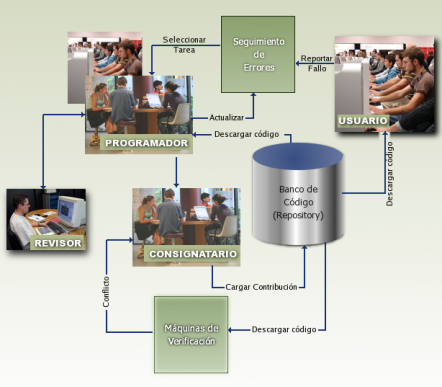
\includegraphics[width=100mm]{proceso_fs.png}
 \caption{Conceptos Básicos en el Desarrollo de Software de Código Abierto}
\label{proceso_fs} 
\end{figure}

Más que una forma de realizar sistemas, se trata de una visión revolucionaria en torno al software como patrimonio de la humanidad y se une a la filosofía del software libre que se expresa en \cite{stallman2002}:

\begin{quote}
“Software Libre” se refiere a la libertad de los usuarios para ejecutar, copiar, distribuir, estudiar, cambiar y mejorar el software. De modo más preciso, se refiere a cuatro libertades de los usuarios del software:

\begin{itemize}
\item La libertad de usar el programa, con cualquier propósito (libertad 0).
\item La libertad de estudiar cómo funciona el programa, y adaptarlo a tus necesidades (libertad 1). El acceso al código fuente es una condición previa para esto.
\item La libertad de distribuir copias, con lo que puedes ayudar a tu vecino (libertad 2).
\item La libertad de mejorar el programa y hacer públicas las mejoras a los demás, de modo que toda la comunidad se beneficie. (libertad 3). El acceso al código fuente es un requisito previo para esto.
\end{itemize}
\end{quote} 

Las aplicaciones más representativas del mundo del software libre como Apache, Mozilla, MySQL, PostgreSQL y el mismo sistema operativo Linux, luego de sus etapas primarias, adoptaron como proceso de desarrollo uno que contravenía en gran manera los fundamentos del control riguroso y ponía el futuro del sistema en manos de la anarquía \footnote{Definida en su sentido positivo como la situación humana en donde es innecesaria e indeseable la autoridad, lo que conlleva a una sociedad libre basada en el respeto mutuo de sus miembros y la cooperación voluntaria entre individuos.\cite{bce}}. Tal como lo propone Linus Torval “la idea es liberar versiones de prueba rápido a menudo, delegar cuanto sea posible, estar abierto hasta el punto de resultar promiscuo”.

Algunos principios fundamentales en este tipo de desarrollo los expone \cite{raymond}:

\begin{quote}
\begin{enumerate}
\item Todo buen trabajo de software comienza a partir de las necesidades personales del programador. (Todo buen trabajo empieza cuando uno tiene que rascarse su propia comezón). 

Esto podría sonar muy obvio: el viejo proverbio dice que "la necesidad es la madre de todos los inventos". Empero, hay muchos programadores de software que gastan sus días, a cambio de un salario, en programas que ni necesitan ni quieren. No ocurre lo mismo en el mundo Linux; lo que sirve para explicar por qué se da una calidad promedio de software tan alta en esa comunidad.
\item Los buenos programadores saben qué escribir. Los mejores, qué reescribir (y reutilizar).

... una importante característica de los grandes programadores es la meticulosidad con la que construyen. Saben que les pondrán diez no por el esfuerzo, sino por los resultados; y que casi siempre será más fácil partir de una buena solución parcial que de cero.
\item "Contemple desecharlo; de todos modos tendrá que hacerlo." cita encontrada en el capítulo 11 de libro The Mythical Man-Month escrito por el célebre Fred Brooks.

Diciéndolo de otro modo: no se entiende cabalmente un problema hasta que se implementa la primera solución. La siguiente vez quizás uno ya sepa lo suficiente para solucionarlo. Así que si quieres resolverlo, prepárate a empezar de nuevo al menos una vez.

\item Si tienes la actitud adecuada, encontrarás problemas interesantes.

\item Cuando se pierde el interés en un programa, el último deber es heredarlo a un sucesor competente.

\item. Tratar a los usuarios como colaboradores es la forma más apropiada de mejorar el código, y la más efectiva de depurarlo.

\item Libere rápido y a menudo, y escuche a sus clientes.

\item Dada una base suficiente de desarrolladores asistentes y beta-testers, casi cualquier problema puede ser caracterizado rápidamente, y su solución ser obvia al menos para alguien.

Dicho de manera menos formal, "con muchas miradas, todos los errores saltarán a la vista". A esto lo he bautizado como la Ley de Linus.

\item Las estructuras de datos inteligentes y el código burdo funcionan mucho mejor que en el caso inverso.

De nuevo Fred Brooks, Capítulo 11: “Muéstreme su código y esconda sus estructuras de datos, y continuaré intrigado. Muéstreme sus estructuras de datos y generalmente no necesitaré ver su código; resultará evidente.” 

\end{enumerate}
\end{quote} 
 
En general un proceso de desarrollo de software libre se basa en el hecho de que el programa puede ser instalado y el código fuente está disponible para cualquier persona. Es decir, la ausencia de barreras en cuanto a la limitación en el uso hace que muchas personas interesas en la funcionalidad que brinda el software lo descarguen y empiecen a utilizarlo. Dando inicio al siguiente ciclo:
\begin{enumerate}
\item El grupo inicial de programadores mantiene un sitio en la red para obtener retroalimentación de los usuarios los cuales reportan fallos, disafuncionalidades y solicitan nuevas características. 

\item Un desarrollador - que puede ser uno de los usuarios, revisa la lista de reportes y decide trabajar en uno específico; para tal efecto descarga la última versión del código fuente la modifica y la envía a un revisor para que este convalide la contribución.

\item La contribución se agrega al código fuente generando una nueva versión del sistema. Esto se realiza sincronizando el código fuente de desarrollo con aquél existente en la bodega de código fuente - repository, la cuál normalmente es un gestionada por un programa para el control de versiones. 

\item Si en algún momento dos programadores están realizando modificaciones a la misma porción de código y pretenden sincronizarlas ocurre un conflicto que deberá ser resuelto siguiendo reglas definidas que habitualmente contemplan el bloqueo de la versión más reciente, el aviso para resolución entre desarrolladores que causan el conflicto o el descarte de las contribuciones.
\end{enumerate}

De esta forma se va refinando el software siguiendo el ciclo mostrado en la figura \ref{proceso_fs}. El grupo de desarrollo se ve aumentado cuando usuarios expertos empiezan a proponer y realizar cambios directos en el código; cuando uno de ellos demuestra tener el suficiente interés y respeto hacia los intereses del software se le asigna el permiso para escribir directamente en la bodega de código.

La creación de la documentación así como de los modelos de requerimientos,análisis, diseño y despliegue siguen el mismo proceso.

\subsubsection{Métodos Ligeros}

Ha principios del milenio un grupo de experimentados desarrolladores, entre los que se encontraban Kent Beck, Alistair Cockburn, Martin Fowler y Dave Thomas, redactaron un manifiesto en el que consignaban los elementos de mayor importancia dentro del desarrollo de sistemas software \cite{beck1999}:
\begin{quote}
Nosotros estamos descubriendo mejores formas de desarrollar software dado que lo creamos y ayudamos a otros a realizar esta tarea. Por medio del trabajo de desarrollo hemos encontrado de gran valor elegir:

\begin{itemize}
\item \textbf{\textit{Individuos e interacciones}} sobre \textit{procesos y herramientas}
\item \textbf{\textit{Software ejecutable}} sobre \textit{documentación profusa}
\item \textbf{\textit{Colaboración del Cliente en el desarrollo}} sobre \textit{contrato de negocios}
\item \textbf{\textit{Respuesta al cambio}} sobre \textit{ceñirse a un plan.}
\end{itemize}

Mientras que existe valor en los elementos de la derecha nosotros valoramos más los elementos de la izquierda.\end{quote}

Con esto sentaban las bases para el despliegue de nuevos métodos de realizar software agrupados bajo el nombre genérico de “ágiles”\footnote{Siendo por definición un método caracterizado por ser liviano y ligero} que se contraponían a los métodos y procesos tradicionalmente rígidos y altamente planificados.

En \cite{koch} se expresan claramente las razones del porqué se desarrollan estos métodos y sus principales características. Los métodos ágiles nacen como respuesta del desarrollador puro al ambiente altamente industrializado y burocrático en el cual transcurren la mayoría de proyectos de desarrollo de software. En estos ambientes es típico el riguroso control que sobre el cumplimiento de cronogramas, planes de trabajo y presupuestos mantienen los denominados \textit{ingenieros de proceso}. El enfoque tradicional se basa en la planificación con la que se trata de \textit{predecir} desde las primeras etapas todos los pormenores del ciclo de desarrollo.

Debido a que los métodos tradicionales tienen fundamento en la ingeniería civil y mecánica, tratan de mitigar los riesgos poniendo un especial interés a las actividades de modelo en especial en las etapas de análisis y diseño; en general relegan a los desarrolladores a etapas de construcción erroneamente consideradas de \textit{cero esfuerzo} intelectual. Los requisitos del software se tratan de fijar desde los inicios del desarrollo, firmandose usualmente un contrato de aceptación de los mismos por parte del cliente. Estos métodos tradicionales siguen los lineamientos de aseguramiento de la calidad por la cual los procesos son eficientemente documentados, controlados, auditados, vigilados y mejorados. Todos esos aspectos hacen que el elemento clave sea el proceso y se relegue a segundo plano el crear productos que en realidad aporten un nuevo valor al cliente.

Para atacar la abrumadora complejidad que añade el proceso al sistema de software, los métodos ágiles proponen cambiar el paradigma \textit{predictivo} - rígido y resistente al cambio; por uno adaptativo que sea flexible y reaccione rápidamente antes cambios inesperados en los requisitos del software. Aquellos que han desarrollado un software de mediana o alta complejidad conocen de primera mano el hecho de que los requisitos no son estáticos, ellos cambian, evolucionan se transforman ya que en sí, no son sino abstracciones de necesidades del mundo real y este no es estático sino que se caracteriza por una fuerte dinámica.

El \textit{cliente también debe ser adaptable} en el sentido de que la mayoría de las veces los requerimientos del sistema los va descubriendo a medida que interactua con él. Una de las premisas de los procesos ágiles es el mantener un contacto permanente con el cliente e involucrarlo en todas las fases del desarrollo. Con esto se logra que el cliente obtenga un software que realmente cope sus intereses y (el cliente) sea consiente de los costos asociados al desarrollo del mismo.

Así como los requisitos cambian durante el desarrollo también lo hacen los recursos y el escenario en el cual se desenvuelve el equipo de trabajo. Para atacar esta característica de los sistemas software, se recomienda \textit{aferrarse a un presupuesto global} pero distribuyéndolo en pequeños presupuestos que solventen las tareas que ha corto plazo realizan los involucrados en el desarrollo.

Es claro con lo expuesto hasta ahora que el enfoque es considerar el desarrollo como una “\textit{carrera de 100 metros planos}” y no como una maratón. En tal sentido se deben gestar planes a corto plazo cuyo objetivo principal sea generar versiones del sistema que puedan ser probadas, corregidas e incrementalmente adicionadas en funcionalidad. Cada plan transcurre en lo que se denomina una iteración la cual usualmente no supera el mes de duración - algunos recomiendan una duración de dos semanas o ménos.\cite{beck1999}

Otro característica de los métodos clásicos, y que atacan los métodos ágiles, es aquella en la cual se considera a las personas como recursos intercambiables mediante la definición de \textit{roles} con funciones específicas y predictivas. Esto hace que las personas - cuyo comportamiento es poco predecible y no lineal \cite{cockburn1999}, tengan una moral baja y descienda su productividad; en el mejor de los casos trabajan con esfuerzo y, si sus condiciones son excelsas, rapidamente abandonan el grupo perdiéndose un activo intangible que repercute negativamente en la calidad global del sistema. Para los metodólogos ágiles el desarrollo se centra en las personas más que en los procesos, considera a cada miembro del grupo como un \textit{ser creativo e irreemplazable}, esto genera un gran cambio en cuanto al método: \textit{no es estático} ni recetario. Evoluciona, se recrea, se adapta y se concerta dentro el grupo de trabajo.

Evidentemente el proceso de desarrollo de software libre maneja los principios promulgados por los métodos ágiles los cuales encuentran quizás su máxima expresión en la Programación Extrema \cite{beck1999}.


\subsubsection{Proceso Unificado}
Según lo expresa \cite{alhir2003}:
\begin{quote}
El Proceso Unificado (UP) es un proceso de desarrollo de software basado en componentes dirigido por casos de uso, centrado en la arquitectura, iterativo e incremental...que utiliza la especificación UML dada por el Object Management Group (OMG) para preparar los esquemas del sistema. El Proceso Unificado es aplicable a diferentes tipos de sistemas de software, incluyendo proyectos de pequeña y larga escala; proyectos que tengan varios grados de complejidad técnica y administrativa, a través de diferentes dominios de aplicación y culturas organizacionales.

El PU nace de la unificación, en 1995, de la aproximación sugerida por Rational Software Corporation y el proceso orientado a objetos de la empresa Objetory AB. Se puede considerar al Proceso Unificado como un modelo de ciclo de vida del proyecto que incluye contexto, colaboraciones e interacciones. El UP es documentado totalmente en el libro “The Unified Software Development Process” escrito por Booch, Rumbaugh y Jacobson, y publicado por Addison- Wesley en 1999.\end{quote} 

Un sistema desde que nace hasta que muere repite el Proceso Unificado en ciclos de desarrollo constituidos por fases secuenciales cuyo objetivo es la producción incremental de liberaciones del sistema, llamadas comúnmente como generaciones del sistema. Cada una de las fases se convierte en un hito principal y esta constituido por pequeños microprocesos denominados \textit{iteraciones}. Habitualmente la numeración de las fases se hace de acuerdo a números enteros mientras que las iteraciones se hacen en números decimales. 

Las fases para el desarrollo de proyectos en el Proceso Unificado son cuatro \cite{jacobson2000}, a saber:

\begin{description}
\item [Fase de Concepción.] Tambien conocida como de inicio. Se centra en el establecimiento de las fronteras, ámbitos, riesgos asociados y visión del proyecto. Determina la viabilidad y los objetivos del proyecto. En esta fase podría tenerse una arquitectura general del sistema que esboze los subsistemas más importantes.

\item [Fase de Elaboración.] Se enfoca en la determinación de la arquitectura y requisitos del sistema; de esta forma se establece su viabilidad técnica. Durante esta fase se construyen los casos de uso críticos y se obtiene una arquitectura refinada del sistema. 

\item [Fase de Construcción] Es en la que se crea la mayor funcionalidad del producto, finaliza con cierta capacidad operativa. Se centra en la construcción del sistema y la arquitectura del sistema se considera estable.

\item [Fase de Transición]. Concluye con la liberación del producto, centrándose en la transición o distribución del sistema a la comunidad o usuario final. 

\end{description}

Dentro de las iteraciones el grupo de trabajo deberá distribuir sus esfuerzos en áreas estratégicas que conduzcan a la mitigación temprana de los riesgos, estás áreas son conocidas dentro del PU como disciplinas, figura \ref{proceso_unificado}:

\begin{itemize}
\item \textbf{Disciplina de administración de cambios en la configuración}, la cual se centra en la administración de la configuración del sistema y de las peticiones de cambios en la misma.

\item \textbf{Disciplina de administración de proyecto.}

\item \textbf{Disciplina de ambiente} que se centra en los ambientes de desarrollo del proyecto, incluyendo los procesos y las herramientas.

\item \textbf{Disciplina de modelado del negocio;} focalizado en la comprensión del negocio que esta siendo automatizado por el sistema capturando dicho conocimiento en un modelo del negocio.

\item \textbf{Disciplina de requerimientos,} necesaria para entender los requerimientos del sistema que automatiza el negocio y captura dichos requerimientos en un modelo de casos de uso.

\item \textbf{Disciplina de diseño y análisis,} centrada en analizar los requisitos y diseñar en sistema capturando tales  conocimientos en un modelo de análisis/diseño.

\item \textbf{Disciplina de implementación} para la implementación del sistema basado en el modelo de implementación.

\item \textbf{Disciplina de pruebas} que maneja las pruebas (evaluaciones) del sistema comparándolos con los requerimientos basándose primordialmente en el modelo de pruebas.

\item \textbf{Disciplina de distribución} encargada de la distribución del sistema basado en el modelo de distribución.
\end{itemize}

Durante la etapa de concepción la mayoría del esfuerzo está distribuido a través del modelo del negocio y la disciplina de requerimientos. 

Durante la fase de elaboración el esfuerzo se distribuye entre las disciplinas de implementación, diseño, análisis y requerimientos. Durante la etapa de construcción el esfuerzo se distribuye entre las disciplinas de análisis, diseño, implementación y pruebas. 

En la fase de transición el esfuerzo se distribuye a través de las disciplinas de prueba y distribución. Obviamente las disciplinas de soporte se distribuyen entre todas las cuatro fases. El objetivo general es producir el sistema, por lo tanto todas las disciplinas nucleares están comprometidas tanto como sea posible para no introducir riesgos en el proceso; esto es, los practicantes son los responsables de determinar cuales disciplinas comprometer y en que momento hacerlo.

En este punto es necesario definir varios conceptos: 
\begin{itemize}
\item \textbf{riesgo} en el Proceso Unificado se concibe como un obstáculo para alcanzar el éxito en la ejecución de una actividad, este riesgo puede estar determinado por características del negocio, humanas o técnicas.

\item \textbf{Iteración} es un paso o rama a través de un ruta hasta cierto destino. Dicho de otra forma es un movimiento planeado que puede ser evaluado para demostrar un progreso tangible dentro de una actividad o proceso, además, de acuerdo a lo citado por \cite{Zavala2000}: “Una iteración es iterativa en el aspecto de que es un acto repetitivo que propende la mejora continua del trabajo. Aditiva en el caso de que el resultado es siempre superior al alcanzado con un solo trabajo y paralela ya que el trabajo puede ser concurrente dentro de la iteración.”

\end{itemize}


\begin{figure}
 \centering
 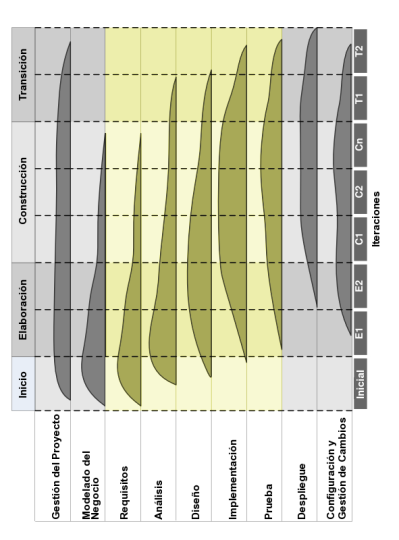
\includegraphics[width=140mm, height=190mm]{pu.png}
 \caption{Ciclo de Desarrollo de un sistema según el Proceso Unificado}
 \label{proceso_unificado}
\end{figure}

Cuando se decantan los \textit{requerimientos}, aquello que el sistema debe cumplir, se está declarando explícitamente los casos de uso los cuales, dado que el Proceso Unificado está manejado por ellos, determinan las iteraciones. De la misma forma en que los casos evolucionan en el marco de las disciplinas regidas por un proceso iterativo, los sistemas evolucionan constantemente con base en iteraciones realizados en el marco de su arquitectura. Incluyendo en la arquitectura todos los elementos, sus colaboraciones e interacciones.  

Resulta pues obvio que la iteración, dado que es un avance demostrable, tiende en últimas a reducir los riesgos inherentes a cada una de las etapas del proceso de desarrollo. Esto ha sido definido por \cite{alhir2003} en su artículo:
\begin{quote}
.. de esta forma las iteraciones confrontan los riesgos derivados de los casos de uso y la arquitectura para alcanzar el éxito en el proyecto, buscando en todo momento reconciliar las fuerza técnicas y del negocio. Una iteración esta acotada en el tiempo con inicio y final fijos en donde una colección de colaboraciones son planeadas, ejecutadas y evaluadas del tal forma que en todo momento se pueda demostrar progreso en el proceso... un caso de uso evoluciona a través de un gran número de iteraciones y a través de cualquier número de disciplinas nucleares en una iteración. La experiencia y aprendizaje obtenido en una iteración evidentemente conduce la aplicación de las próximas iteraciones dentro del proceso..\end{quote} 

La iteración se convierte en el hito más importante para asegurar el crecimiento continuo y el aseguramiento de la calidad total dentro del sistema que se está desarrollando. Las iteraciones marcan totalmente el ciclo de desarrollo del SITEM que utiliza una aproximación iterativa propuesta por el Proceso Unificado.

\section{UML: Lenguaje de Modelado Unificado}

Independiente del modelo utilizado para la construcción y gestión del desarrollo del sistema se requiere que la comunicación entre los diferentes integrantes del grupo de desarrollo sea efectiva. Se hace indispensable que todo el equipo utilice y entienda un lenguaje consistente y unificado con el cual expresen claramente sus ideas y desde el cual puedan marcar claramente las directrices a seguir. El lenguaje de Modelado Unificado, UML por sus siglas en inglés, brinda las características tanto sintácticas como semánticas para lograr caracterizar lógicamente cualquier tipo de software permitiendo ser utilizado en cualquier etapa del diseño y es especialmente útil en aquellos desarrollos enfocados a objetos.

El Lenguaje de Modelado Unificado es definido por el \textit{Object Management Group}\footnote{La página del OMG (www.omg.org) describe la organización como un consorcio de la industria de la informática, sin ánimo de lucro, con caracter internacional y de membresía abierta. Los diferentes grupos de trabajo del OMG desarrollan estándares en un rango amplio de tecnologías.}:
\begin{quote}
UML es un lenguaje visual para la especificación, construcción, y documentación de los artefactos de un sistema. Es un lenguaje de modelado de propósito generalque puede ser usado con la mayoría de los métodos orientados a objetos y a componentes; que puede ser aplicado a todos los dominios de aplicación (p.e., salud, finanzas, telecomunicaciones, aeroespacial) y plataformas de implementación (p.e., J2EE, .NET). \end{quote} 

En \cite{jacobson2005} se recalca que UML es usado para entender, diseñar, buscar, configurar, mantener y controlar la información acerca de los sistemas.

Con UML se crean artefactos con información acerca de la estructura - o vista estática- y el comportamiento - o vista dinámica- de un sistema. Cada vista del sistema se modela como una colección de objetos que interactuan, es decir, que tienen interfaces y relaciones entre ellos perfectamente definidas. Fruto de tal relación entre objetos el sistema ofrece una funcionalidad o cumple un objetivo que es de interés.
\section{Portales de Información y Conocimiento}

Antes de la explosión de servicios a través de la Internet, los portales basados en aplicaciones web estaban recomendados solo para organizaciones que por su complejidad (en tamaño ó geografía) necesitaran de un sistema tecnológico para que todo su personal pudiese tener acceso a la información en forma compartida y simultánea. Sin embargo, fundamentado en el crecimiento del uso de Internet\footnote{El porcentaje de la población con acceso a Internet en Colombia a crecido de un 2,1\% en el año 2000 a un 15,8\% en el 2007, según la Comisión de Regulación de Telecomunicaciones.} surgue la necesidad de la sociedad por mantener cierto orden en la corriente de bytes y grupos de usuarios con intereses de información comunes empiezan a conglomerarse alrededor de portales temáticos no organizacionales.

Un portal de información no es, en esencia, una fuente nueva de información; es una vista de la información existente que dispuesta en una forma ordenada se convierte en una herramienta de conocimiento extraordinariamente poderosa permitiendo poner al descubierto información valiosa que se enmascaraba entre otra no menos interesante – Data Mining.
Dentro de las múltiples ventajas que ofrece el portal, es que proporciona la facilidad de obtener información actualizada a muy corto plazo, lo que es indispensable para la óptima toma de decisiones. Dicha información esta disponible, en condiciones óptimas,  veinticuatro horas al día, trescientos sesenta y cinco días del año, permitiendo así acceder a los datos que se necesitan de acuerdo con la disponibilidad singular de tiempo y apoyar la toma de decisiones bajo cualquier circunstancia y lugar.

Gran cantidad de organizaciones y grupos de usuarios están explotando el uso de los portales creando y transformando servicios y procesos tradicionales convirtiéndolos en servidores de autoservicio, pudiendo así dedicarse a aquellos de mayor valor agregado a la organización, el personal o el grupo de investigación. 

\subsection{Beneficios y obstáculos para la implementación de portales basados en aplicaciones web.}

Las facilidades que proporciona la tecnología, permite que el portal sea accedido a través de numerosas opciones, esto es a través de computadoras de escritorio y portátiles integradas a la red interna de la organización, a través de Internet por redes de banda ancha y estrecha y de los diversos medios inalámbricos como son las tecnologías celular, WiFi, WiMax, BlueTooh por intermedio de PDA, celulares y equipos de cómputo en redes WLAN.

Debido a la estructura del portal, se tiene una fuerte correlación entre diversas aplicaciones que nos permiten analizar interrelaciones que serían realmente complejas y tardadas si no se contara con ellos. Sin embargo, es importante recalcar más que los beneficios los problemas potenciales. De hecho en el éxito de un portal están enfocados factores clave que tienen beneficios y problemas asociados.

\begin{description}
 \item[Factor Humano] Los individuos adaptan los procesos de información en diferentes maneras. 
 \item[Factor Tecnológico] Intranets, pueden ser costosas y poco efectivas si la organización no tiene la tecnología necesaria para construirlas.
 \end{description} 

La principal ventaja obtenida al construir y mantener un portal basado en aplicaciones web es mejorar la eficiencia y efectividad en la comunicación de los miembros de una organización o un grupo de usuarios, lo que aumenta la objetividad en la toma de decisiones y la transferencia de conocimiento. Todo lo anterior se maximiza si el portal se concibe como fruto de un proceso de investigación en donde todos sus componentes y servicios se construyen, mantienen, distribuyen e integran de acuerdo a los requerimientos de los usuarios finales\cite{sarmento2005}.

Una de las características importantes de los portales es que en un sólo lugar - y con un mecanismo de acceso unificado, los usuarios pueden acceder a las aplicaciones. Esta integración con aplicaciones y servicios orientados al trabajo colaborativo hacen que trascienda los límites de un mero repositorio organizacional - que permite el autoservicio de requerimientos y extracción de información básica - y lo convierte en una herramienta de administración del conocimiento, útil para la toma de decisiones.

Las novedosas tecnologías que convergen en Internet permiten que la información sea personalizada y dirigida de tal forma que se potencian ciclos de creación, captura y diseminación de conocimiento necesarios para el crecimiento de los activos intangibles de los grupos y organizaciones. Así los portales convierten la información en valor, ya que eliminan las barreras de distancia y disponibilidad de información, reduciendo costos conectando a múltiples personas en diversos sitios al mismo tiempo.

La tabla \ref{beneficio} muestra los principales beneficios potenciales de desplegar los portales de información y conocimiento dentro del quehacer de las organizaciones, los grupos de trabajo y las comunidades de práctica.

\begin{table}
\begin{center}
\begin{tabular}{|l|}
\hline
\textbf{Beneficios Humanos (suaves)}\\
\hline
Provee estructura de soporte 24 hrs.\\
Servicio centrado en el usuario.\\
Medio ambiente amigable.\\
\hline
\textbf{Beneficios Físicos y capitales (beneficios fuertes)}\\
\hline
Creación medioambiente libre de papel.\\
Mejorar eficiencia y efectividad.\\
Reducción de costos.\\
Menores tiempos en consecución de información.\\
\hline
\textbf{Beneficios estratégicos}\\
\hline
Creación de herramientas innovadoras de apoyo.\\
Proveer información a tiempo real.\\
Apoyo a proceso de negocios de reingeniería\\
Apoyo a los ciclos de creación, captura y diseminación de conocimiento.\\
Aumento de Capital intangible.\\
Formalización del \textit{Know-How}.\\
\hline
\end{tabular}
\caption{Algunos Beneficios Potenciales al Implementar un Portal}
\label{beneficio} 
\end{center}
\end{table}

Los riesgos que se afrontan también son enormes y pueden llevar al traste cualquier política o proyecto de desarrollo; la tabla \ref{riesgos} muestra algunos de los más importantes que deben ser minimizados.

\begin{table}
\begin{center}
\begin{tabular}{|l|}
\hline
\textbf{De tipo Humano (Fuertes)}\\
\hline
Indiferencia de la administración.\\
Sobrevaloración del papel de las TIC\\
Dirección centrada en el capital financiero\\
Estructuras organizacionales conservadoras.\\
Micropoderes y feudos organizacionales autogestionados.\\
Ignorancia y/o resistencia respecto al uso de TIC.\\
Resistencia a estandarizar la información.\\
Resistencia a compartir información/conocimiento.\\
\hline
\textbf{Riesgos Físicos/Capital}\\
\hline
Procesos orientados a la técnica y no multidimensionales.\\
Carencia de capital(TIC marginales).\\
Dificultad de integración de tecnología nueva y la existente.\\
Ausencia de inter, trans y multidisciplinariedad.\\
\hline
\textbf{Riesgos tecnológicos (Débiles)}\\
\hline
Estándares propietarios.\\
Redes de interconexión da baja velocidad.\\
Alta relación Consumo/Adopción de tecnología.\\
\hline
\end{tabular}
\caption{Algunos riesgos Potenciales al Implementar un Portal}
\label{riesgos} 
\end{center}
\end{table}

\subsection{Ciclo de Vida de los Portales}
Los portales como representación sistemática del quehacer de un grupo humano evoluciona en la medida que dicho grupo mejora su conocimiento de las relaciones entre sus miembros y el entorno que los rodean. En general pueden determinarse cinco macro-etapas~\cite{egovernment} que aumentan gradualmente su funcionalidad basado en el  conocimiento organizacional y la interrelación de usuarios a través del Portal:

\begin{description}
\item[Presencia Emergente]
Esta es la etapa primaria por la que pasa un portal en donde su funcionalidad es la de distribuir información interesante para un grupo de usuarios, el cual es totalmente caracterizado por el grupo de personas que construye - en todas sus dimensiones, el portal. Dichos usuarios no intervienen directamente en la estructura del Portal el cual complementa sus servicios por medio de enlaces y dependencia a otros portales temáticamente relacionados.

\item[Presencia Mejorada] 
Los usuarios pueden determinar en cierto grado la navegación a través de búsquedas en el archivo del sitio. Un portal en esta etapa presentará gran cantidad de información que usualmente se agrupa por áreas temáticas. Los mapas del portal se distribuyen profusamente con el fin de guiar a los usuarios en su tránsito por el mismo y usualmente un sistema básico de ayuda prediseñada esta disponible.
 
\item[Interacción]
Los portales registran a sus usuarios. Se implementan herramientas en línea como las salas de charla - chat, las listas de correo y los foros; se realiza capacitación básica por medio de seminarios basados en contenidos y se hace uso extensivo de recursos multimediales. La ayuda es síncrona o asíncrona pero ágil lo que fomenta una depuración y actualización de la información contenida en el portal.

\item[Transacción] 
Los usuarios realizan operaciones a través del portal. El comercio electrónico, la gestión de contenidos, la personalización de los ambientes del portal, búsquedas semánticas y el despliegue de servicios avanzados - cursos, blogs, etc; caracterizan esta etapa.

\item[Transformación] 
La etapa más avanzada de los portales en donde se han estructurado comunidades de práctica sobre temas concretos que potencian los ciclos de conocimiento mediante las herramientas brindadas por el portal. Se observa una jerarquía \textit{ad hoc} de usuarios con base en su aporte. Ellos mismos generan contenido que es convalidado por la comunidad y los administradores técnicos limitan sus funciones a aquellas relacionadas con mantener operativa la plataforma tecnológica. Las transacciones y el contacto en tiempo real son rutinarios. Las aplicaciones son de conocimiento general y el nivel de inmersión en el portal es alto.
\end{description}


\subsection{Aplicaciones Web}

También conocidas como \textbf{WebApps} son, en su concepción más básica, aplicaciones que responden a peticiones realizadas por un usuario por medio de un navegador (cliente) y ejecutan la lógica del programa en un servidor. Las aplicaciones web usualmente interactúan con sistemas de bases de datos y distribuyen los resultados de sus operaciones en lenguajes estándar tales como HTML, SMIL, XML,  RDF, SVG, etc.\cite{jackson2005}. Las WebApps también se pueden encontrar en ambientes diferentes al modelo cliente - servidor\cite{bos2004}. 

Entre las características de las aplicaciones web se destacan\cite{bos2004}:

\begin{itemize}
\item \textbf{No requieren instalación.} En general las aplicaciones web no necesitan ejecutar rutinas de instalación en las máquinas cliente. Quizás en algunos lenguajes sea necesario la preparación de un ambiente específico de trabajo que en la mayoría de las veces es de acceso público.

\item \textbf{Accesibilidad.} Las aplicaciones web se despliegan desde de una página web. Los protocolos usados son estandarizados y abstraen fácilmente las capas de aplicación de las de diseño y datos.

\item \textbf{Facilidad en el Desarrollo.} Los lenguajes usados son de alto nivel, con un buen soporte para cadenas de caracteres, diferentes tipos de datos y con facilidades para la programación orientada a objetos. La mayoría de ellos con sintaxis similares y herramientas de desarrollo gratuitas de fácil adquisición. 

\item \textbf{Independencia de la Plataforma.} Las \textit{WebApps engines} implementan el modelo de capa intermedia lo que permite que las diferentes WebApps puedan ser desplegadas sobre diferentes plataformas sin detrimento de su funcionalidad. El uso de métodos genéricos definidos en interfaces de programación (API) ayuda en gran manera a garantizar esta característica.

\item \textbf{Seguridad.} No obstante la facilidad de acceso de la WebApp, estas pueden implementar rutinas avanzadas que brindan ambientes transaccionales seguros aislados del sistema de archivos y configuración del sistema en donde se alojan. El intercambio de información cifrada por la red y la integración con la seguridad de los servidores de bases de datos forman un contexto de alta seguridad.

\item \textbf{Privacidad.} Las WebApps pueden operar fácilmente sobre una Plataforma de Preferencias de Privacidad debido a que la mayoría de los motores están habilitados para soportar el protocolo \textbf{P3P}.

\item \textbf{Almacenamiento Persistente.} Tanto en el cliente - a través de archivos texto para el manejo de sesiones; como en el servidor de base de datos.

\item \textbf{Integración.} Las aplicaciones Web pueden brindar sus servicios - u obtener uno determinado, a través de interfaces claras y definidas en las denominadas redes de servicios Web.
\end{itemize}

\input{Federación de Aplicaciones}
\chapter{OpenSITEM: Sistema Federado de Aplicaciones para la Caracterización de Nodos Potenciales de Redes de e-salud}

\textbf{OpenSITEM }es un sistema federado de aplicaciones de software libre o de código abierto que provee herramientas para analizar datos e información de los siguientes elementos que son de interés para la descripción - y definición de capacidad de, nodos potenciales de redes de e-salud: entidades de salud, servicios médicos, tecnologías de interconexión, operadores de telecomunicaciones, equipos médicos, organizaciones, profesionales, estándares, pacientes, enfermedades, medicamentos y proyectos. Provee un ambiente para apoyar las tareas de las comunidades de práctica involucradas en la investigación, el diseño, mantenimiento, desarrollo e implementación de redes de eSalud. Tuvo su génesis conceptual en la primera fase del Proyecto Telemedicina Bogotá como solución a la necesidad de administrar los resultados del estudio de campo realizado a las entidades e instituciones de salud y los operadores de Telecomunicaciones en la ciudad de Bogotá.

Su principal objetivo es: Implementar un sistema que permita la definición, categorización y caracterización de nodos potenciales de redes de eSalud, para apoyar las actividades básicas de los \textit{trabajadores del conocimiento} en el área de la telemedicina del grupo GITEM\footnote{Conformado por profesionales y estudiantes de la Universidad Distrital así como por profesionales de las diferentes instituciones que han participado en los diferentes estudios de campo.}  ofreciéndoles, además de un repositorio de datos, herramientas que facilitan las tareas de capturar, extraer, organizar, analizar, encontrar, sintetizar, distribuir y compartir información y conocimiento de nodos potenciales de las redes de eSalud. OpenSITEM cuenta con herramientas para poder  actualizar el estado de los nodos definods en el modelo base así como para la definición de nodos y categorías inéditas del Sistema de Salud de Bogotá Distrito Capital. El modelo base de nodos y categorías se construye a partir del estudio de campo realizado por el grupo de investigación, haciendo especial énfasis en los requerimientos de eSalud que se definieron en esa época.Con OpenSITEM se sistematiza los resultados de los estudios de campo emprendidos por el grupo de investigación GITEM y se constituye una plataforma para gestionar los datos de nodos potenciales de redes de eSalud. Contribuye a disminuir el tiempo de adquisición, análisis y despliegue de la información.  
\begin{figure}
 \centering
 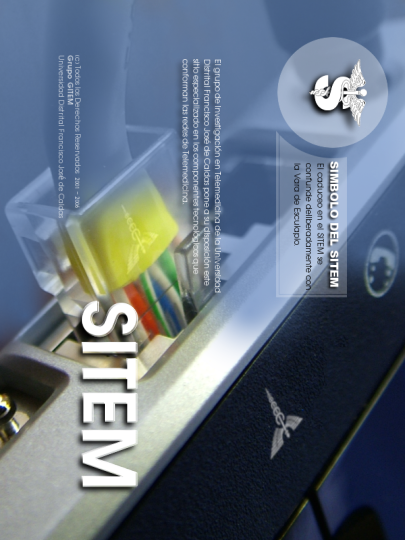
\includegraphics[width=142mm, height=190mm]{sitem_principal.png}
 \caption{Imagen en el año 2017 de la página principal de OpenSITEM}
 \label{pantalla_sitem}
\end{figure}

El proceso de integración del sistema\footnote{OpenSITEM es un sistema federado de aplicaciones.} está basado en métodos ampliamente conocidos \cite {balduino2010}, \cite{koch},\cite{jacobson2000},\cite{larman2004}. Para el diseño de los módulos inéditos se ha tenido en consideración principios, patrones y antipatrones, tratando de minimizar los riesgos asociados a la mala calidad del software.

OpenSITEM hace uso extensivo de aplicaciones existentes, marcos de trabajo, bibliotecas, APIs, servicios web y plantillas, lo que ha permitido lograr un alto grado de funcionalidad específica. Los módulos propios\footnote{En referencia a la autoría, no al carácter de código abierto.} - aquellos que hacen parte de la suite desarrollada por GITEM - se implementan sobre el framework OpenSARA \footnote{Diseñado y construido por GITEM. OpenSARA es un producto de este proyecto y se ha usado en otros dominios tanto en la Universidad Distrital (sistema de gestión de inventarios, sistema de consultas a comunidades, sistema de evaluación para acreditación, entre otros), como por algunas empresas del sector TI (OpenKyOS).}.

\section{Módulos Funcionales}

OpenSITEM- incluyendo las aplicaciones de terceros y las desarrolladas por GITEM, ofrece los siguientes módulos base:

\begin{table}[]
\centering
\caption{Módulos base de OpenSITEM}
\label{tabla_modulos_opensitem}
\begin{tabular}{lcl}
\rowcolor[HTML]{C0C0C0} 
\multicolumn{1}{c}{\cellcolor[HTML]{C0C0C0}\textbf{Módulo}} & \textbf{Elaboración} & \multicolumn{1}{c}{\cellcolor[HTML]{C0C0C0}\textbf{Nombre}}            \\
Motor de Federación de Aplicaciones                         & Propia               & OpenSITEM-FE                                                           \\
Motor de recomendación                                      & Propia               & OpenSITEM-RS                                                           \\
Gestión de Nodos                                            & Propia               & OpenSITEM-NM                                                           \\
Diseñador de Redes                                          & Propia               & OpenSITEM-ND                                                           \\
Analizador de Redes                                         & Propia               & OpenSITEM-NA                                                           \\
Gestión de Encuestas                                        & Propia               & OpenSITEM-PM                                                           \\
Inteligencia de Negocio                                     & Tercero              & Knowage                                                                \\
Sistema de Información Geográfica                           & Tercero/Propia       & \begin{tabular}[c]{@{}l@{}}Cesium\\ qGIS\\ Leaflet\end{tabular}        \\
Gestión Documental                                          & Tercero              & Alfresco                                                               \\
Gestión de Reportes                                         & Tercero/Propio       & \begin{tabular}[c]{@{}l@{}}Reportico\\ Varias bibliotecas\end{tabular}
\end{tabular}
\end{table}

\subsection{Características innovadoras de OpenSITEM}


OpenSITEM presenta innovaciones en diferentes dominios:

\begin{itemize}
 \item Dominio de Aplicación: Desarrolla un motor y un proceso para la federación de aplicaciones. 
 \item Dominio de arquitectura: Propone un modelo de arquitectura para nodos en redes de eSalud.
 \item Dominio de utilidad: Implementa una plataforma para soportar flujos de trabajo de investigadores del GITEM. En el mercado no existe una herramienta que de manera unificada cumpliera con el modelo de requerimientos definido.
 \item Dominio social: Tanto el framework (OpenSARA) como los módulos de OpenSITEM están disponibles en repositorios públicos y cobijados por licencia de código abierto. El framework ya se ha utilizado por equipos de trabajo externos al grupo GITEM. Se tiene presupuestado que la fase IV del proyecto (transición) permita que los datos también sean abiertos. 
\end{itemize}


\section{Descripción de la Arquitectura de OpenSITEM}

OpenSITEM es una aplicación federada de arquitectura orientada a servicios, con características como las descritas en {earl2017}. La integración es realizada por un motor que permite el intercambio de mensajes y la sincronización de sesiones entre los diferentes aplicativos federados sin llegar a considerar una arquitectura de Bus de Servicio Empresarial (ESB por sus siglas en inglés)\footnote{Aunque existen ESB de corte empresarial tales como Mule, WSO2, Apache Service Mix o similares, el análisis de utilidad mostró que la mayoría de funcionalidades que ofrecen nunca serían utilizadas y entonces se optó por la simplicidad arquitectónica y evitar la tarea recurrente de configuración y administración del ESB. Ver el anexo \ref{appendix:lista_de_chequeo_ESB}.} 

El presente informe describe la arquitectura general de OpenSITEM y de los módulos inéditos realizados en el marco del proyecto. Las aplicaciones federadas construidas por terceros se abstraen, visibilizando únicamente las interfaces provenientes de las API o de los servicios web de adaptación. 

\subsection{Arquitectura General}

La descripción de la arquitectura sistema (AD) se realiza con base al modelo conceptual definido en \cite{ISO42010}. Dada la extensión de los artefactos, se presentan aquellos apartes de la AD que a juicio de los autores se consideran relevantes para explicar las propiedades fundamentales.

\subsubsection{Interesados e Intereses}

El proyecto considera una aplicación inédita de la cual no se encontró referente de modelo de dominio. En este escenario se vuelve particularmente importante la identificación de los interesados los cuales están enfocados a los investigadores del grupo GITEM que participan en proyectos relacionados con las redes de eSalud, así como expertos en el diseño de redes de telecomunicaciones y de prestación de servicios médicos.

Los mecanismos utilizados para la identificación fueron:

\begin{itemize}
 \item Entrevistas Directas: Realizadas en su mayoría durante la primera iteración de la fase de inicio. Se definió una entrevista base, anexo \ref{appendix:entrevista_posible_interesado}.
 \item Reunión Presencial: De duración fija (30 minutos) y con agenda previa \footnote{La agenda en las reuniones de identificación fue simple. Se buscaba tener una idea de quienes eran los interesados representativos de los diferentes roles que existen en el grupo.}.
 \item Matriz de identificación: En donde se consignaron las evaluaciones de los atributos de liderazgo, poder de decisión, nivel de interés en el proyecto, conocimiento, actitud ante el proyecto (oposición, neutralidad, soporte), procedencia (externa o interna - GITEM, Universidad). 
\end{itemize}

La siguiente tabla muestra el resultado del proceso de identificación:


\begin{table}[]
\centering
\caption{Principales Interesados}
\label{tabla_principales_interesados}
\begin{tabular}{ll}
\multicolumn{1}{c}{\textbf{Interesado}} & \multicolumn{1}{c}{\textbf{Intereses Principales}}                                                                                                                                                                                                                                                                                                                                                                                                                                                                                                                                                                                   \\
Asistente de Investigación Hospital     & \begin{tabular}[c]{@{}l@{}}*  Ingresar y corregir la información recopilada en el estudio de campo.\\ * Elaborar informes a partir de la información ingresada utilizando diferentes filtros y formatos.\\ * Generar una plantilla del informe de investigación que cumpla con los parámetros exigidos por la Universidad.\\ * Registrar las evidencias de las visitas de campo y demás entregables que exige el proyecto.\\ * Gestionar el proyecto de caracterización de los hospitales.\\ * Visualizar geográficamente algunos atributos del hospital (ubicación, zona de influencia, procedencia de pacientes, etc)\end{tabular} \\
Analista en Proyectos eSalud del GITEM  & \begin{tabular}[c]{@{}l@{}}* Analizar la información de diferentes nodos (centros de atención en salud, proveedores de telecomunicaciones, profesionales de salud, pacientes, equipos médicos, servicios médicos, servicios de educación, etc)\\ * Evaluar la potencialidad de los nodos para pertenecer a una red de eSalud.\end{tabular}                                                                                                                                                                                                                                                                                           \\
Diseñador de redes de eSalud            & \begin{tabular}[c]{@{}l@{}}* Diseñar redes de eSalud a partir de la interconexión de nodos de prestadores de salud.\\ * Evaluar la potencialidad de las redes diseñadas.\end{tabular}                                                                                                                                                                                                                                                                                                                                                                                                                                                \\
Experto en nodo                         & \begin{tabular}[c]{@{}l@{}}* Ingresar y corregir información relacionada con el nodo.\\ * Elaborar informes a partir de la información ingresada utilizando diferentes filtros y formatos.\end{tabular}                                                                                                                                                                                                                                                                                                                                                                                                                             
\end{tabular}
\end{table}

\subsubsection{Punto de Vista Estructural}

La estructura de OpenSITEM se presenta principalmente desde tres puntos de vista:

\begin{itemize}
 \item Punto de Vista de Negocio (\ref{punto_negocio}): Con los grupos de actores, roles generales, servicios de negocio y procesos de negocio.
 \item Punto de Vista de Aplicación (\ref{punto_aplicacion}): Con los grupos de Servicios de aplicación y Módulos de Aplicación (federadas y nativas\footnote{Una aplicación federada es aquella que mayormente ha sidos desarrollada por equipos externos, mientas que una aplicación nativa es la que mayormente ha sido desarrollada por integrantes de GITEM.}).
 \item Punto de Vista Infraestructura (\ref{punto_infraestructura}): Con los grupos de Servicio de Infraestructura y Componente de Infraestructura.
\end{itemize}

\begin{figure}
 \centering
 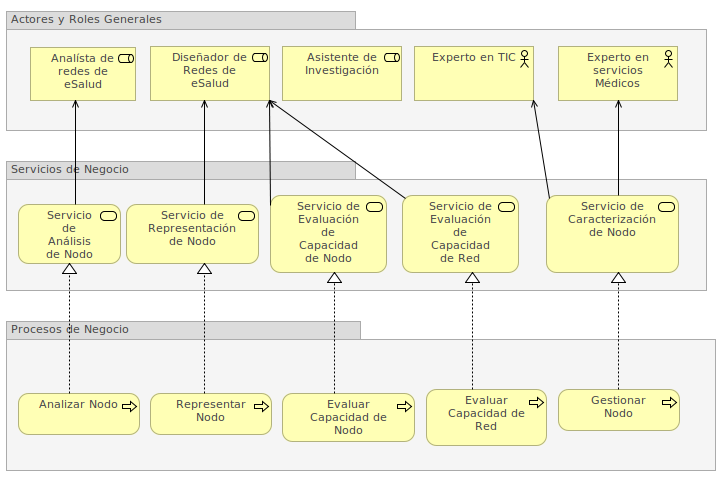
\includegraphics[width=120mm]{negocio_vista_por_capas.png}
 \caption{Punto de Vista de Negocio - Vista Conceptual por Capas}
 \label{punto_negocio}
\end{figure}

\begin{figure}
 \centering
 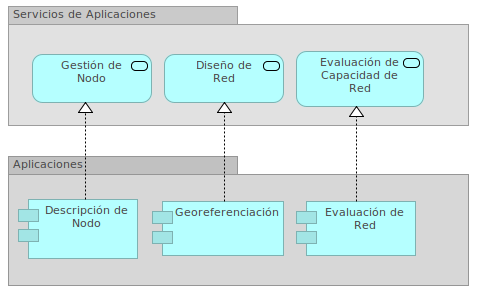
\includegraphics[width=120mm]{punto_aplicacion.png}
 \caption{Punto de Vista de Aplicación - Vista Conceptual por Capas.}
 \label{punto_aplicacion}
\end{figure}

Las aplicaciones nativas se denotan por las iniciales de cada módulo. Por ejemplo el motor de federación (Federation Engine) se conoce como OpenSITEM-FE, el gestor de nodos (Node Management) como OpenSITEM-NM, etc.

\begin{figure}
 \centering
 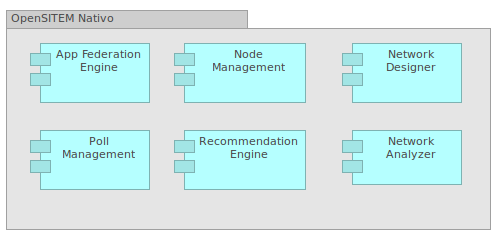
\includegraphics[width=120mm]{opensitem_nativo.png}
 \caption{Punto de Vista de Aplicación - Aplicaciones nativas de OpenSITEM.}
 \label{punto_aplicacion}
\end{figure}


\begin{figure}
 \centering
 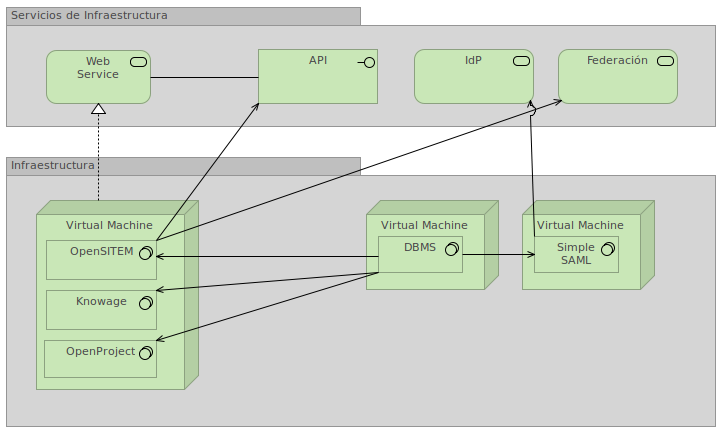
\includegraphics[width=120mm]{punto_infraestructura.png}
 \caption{Punto de Vista de Infraestructura - Vista Conceptual por Capas.}
 \label{punto_infraestructura}
\end{figure}


\subsubsection{Punto de Vista de Comportamiento}

\paragraph{OpenSITEM-FE: Motor de Federación de Aplicaciones}

OpenSITEM no es un sistema de federación universal de aplicaciones. Integra aplicaciones que expongan su funcionalidad a través de interfaz de programación de aplicaciones (API) o de servicios web, utilizando protocolos de la pila TCP/IP con representación basada en XML o JSON. Por esta razón - y por las mostradas en el anexo \ref{appendix:lista_de_chequeo_ESB}; se prescindió de emplear una solución ESB y se diseñó un motor de integración con la siguiente funcionalidad:
\begin{itemize}
 \item Evaluación de Federación: Servicio que se encarga de recibir el mensaje proveniente de una aplicación - a través de un servicio web general, y definir si dicho mensaje hace parte de una transacción que es necesario ser federada. En el contexto de OpenSITEm, se dice que una transacción es federada cuando luego de su ejecución debe ``disparar'' transacciones en uno o varios sistemas diferentes.
 \item Acceso a Aplicación: Servicio por el cual un usuario adquiere las credenciales para acceder o consumir un servicio específico de una aplicación federada.
 \item 	Registro de transacción: Servicio específico por aplicación federada que se encarga de consumir un servicio web, y objetivo es realizar una transacción en una aplicación. 
\end{itemize}

\begin{figure}
 \centering
 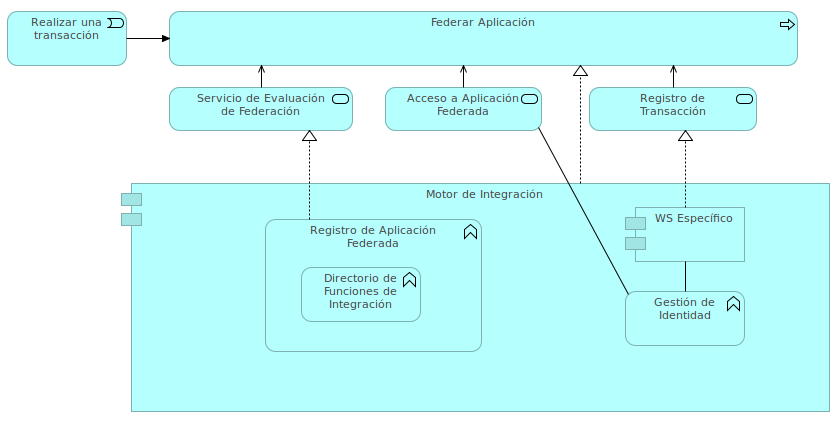
\includegraphics[width=120mm]{motor_integracion_vista_comportamiento.png}
 \caption{Punto de Vista de Comportamiento - Modelo General del Motor de Federación de Aplicaciones.}
 \label{punto_infraestructura}
\end{figure}


\subsubsection{Punto de Vista de Distribución}

Tanto OpenSITEM como cada una de las aplicaciones federadas están desplegadas en una infraestructura virtualizada. Aunque al momento de elaborar este informe se está trabajando en migrar a contenedores, la tecnología que se empela esta 100\% relacionada con máquinas virtuales.

\begin{figure}
 \centering
 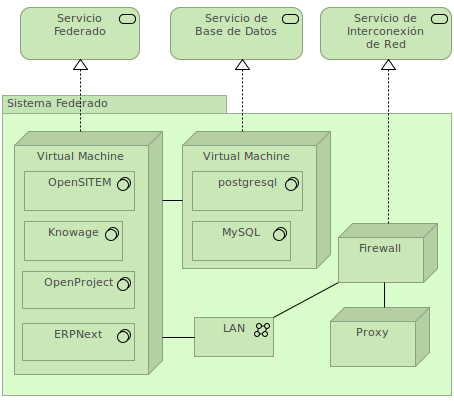
\includegraphics[width=120mm]{openSITEM_Vista_Distribucion.png}
 \caption{Punto de Vista de Distribución.}
 \label{punto_infraestructura}
\end{figure}

En un plano técnico, cada una de las instancias utiliza un sistema operativo GNU/Linux con distribución Centos.


\subsection{Gestión de nodos}

El módulo de gestión de nodos se puede considerar como un directorio enriquecido de los objetos con potencialidad de pertenecer a una red de eSalud. En OpenSITEM se considera que este es el nivel ontológico de mayor abstracción y constituye lo que denominamos el \textit{Catálogo de Nodos}.




\subsection{Motor de Recomendación}


\subsection{Gestión de Encuestas}






\section{Modelo de Nodos}

Como se presentó anteriormente, el motor de gestión de nodos permite la definición de cualquier tipo de nodo. No obstante, el equipo de trabajo ha definido un modelo base de nodos que se consideran el conjunto reducido que permite describir los elementos primordiales \footnote{En es te caso el carácter de \textit{primordial} fue definido por el grupo de interesados del GITEM.}

















\subsubsection{Subsistema Entidades de Salud} 
Este subsistema, figura \ref{entidades}, se creó para gestionar los datos recopilados en el estudio de campo realizado por el grupo GITEM en el marco del proyecto del Sistema de Gestión de Salud para el Distrito Capital fases I y II. Es por ende el subsistema base para el SITEM y su objetivo principal es la gestión de información referente a las entidades de salud en el entorno colombiano enfocándose en tres redes principales: la red de especialidades médicas, la red de comunicaciones y la red de atención.

\begin{figure}
 \centering
 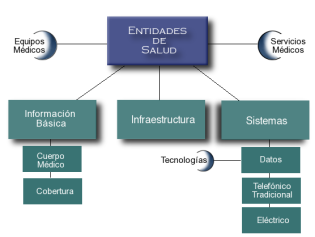
\includegraphics[width=80mm, height=52mm]{entidades.png}
 \caption{Arquitectura Básica del Subsistema Entidades}
\label{entidades}
\end{figure}

La información disponible en el subsistema puede ser administrada por cada una de las entidades prestadoras de servicios de salud, de tal forma que se cree gradualmente un catálogo flexible para conocer el estado actual de las entidades y su potencialidad para ser parte en redes que presten servicios de salud a distancia usando TIC. Por defecto, las entidades se asocian a la arquitectura de red de la secretaría de Salud de Bogotá pero por medio del módulo denominado \textit{redes de atención} se puede crear fácilmente cualquier prototipo de red jerárquica de atención \cite{yellowlees}.

\subsubsection{Subsistema Tecnologías de Interconexión} 
Administra información relacionada con las tecnologías y protocolos de interconexión disponibles en las redes de acceso y transporte. Estas tecnologías se ordenan principalmente sobre el modelo de referencia OSI pudiéndose crear  - desde el módulo de arquitecturas, cualquier otro tipo de modelo. En la actualidad se tiene como alternativa de clasificación el modelo de TCP/IP. Es una guía técnica que muestra la información de las capas físicas, de enlace y de red en formatos básicos- o de características generales; e intermedios - o de características técnicas.

El objetivo principal que se persigue con la implementación de este subsistema es proveer a los analistas información para la revisión sistemática de las diferentes opciones que brindan los fabricantes de dispositivos y así proyectar redes que sean técnicamente viables. La información se estructura de acuerdo a indicadores cualitativos y cuantitativos que permiten evidenciar el carácter de interoperabilidad, impacto y permanencia de la tecnología en el mercado. 

\subsection{Subsistema Equipos y Tecnologías}
Información técnica sobre los diversos equipos y tecnologías usadas en Telemedicina. Posee secciones para la gestión de Información especializada de proveedores y fabricantes, así como la gestión de especificaciones técnicas, funcionales y físicas de los equipos.

Combinado con los demás subsistemas provee un mecanismo eficiente para realizar auditorías \textit{ex-ante} en redes tecnológicas, valorando alternativas de intercambio y reposición en los nodos.

\subsubsection{Subsistema Operadores de Telecomunicaciones}

\begin{figure}
 \centering
 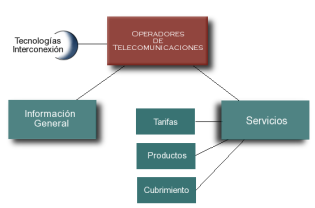
\includegraphics[width=80mm, height=52mm]{operadores.png}
 \caption{Arquitectura Básica del Subsistema Operadores de Telecomunicaciones}
 \label{operadores}
\end{figure}

Contiene información relacionada con operadores de telecomunicaciones, figura \ref{operadores}, con énfasis en las características técnicas de los servicios que ofrecen, su cobertura y tarifas. Brinda a los analistas información comparativa entre operadores lo que permite determinar las ventajas y desventajas entre diferentes opciones de interconexión, de acuerdo a los servicios médicos que se quieren implementar. Este módulo se complementa con la información de los subsistemas de tecnologías de interconexión y servicios médicos, así como de la información de dominio público que muestra el \textit{Sistema de Información Unificado para el sector de las Telecomunicaciones} mantenido por la Comisión Reguladora de Telecomunicaciones.

\subsection{Subsistema Organizaciones y Proyectos} 

Posee herramientas informáticas para la gestión de información de proyectos nacionales y de la región en el ámbito de la Telemedicina, la Telesalud y la Tele - educación en medicina. 

Incluye secciones para la gestión de los datos correspondientes a organizaciones y grupos de investigación que trabajen en el área de la Telemedicina.  Este subsistema es uno de los pilares del SITEM pues en él se despliegan aplicaciones que fomentan el trabajo en grupo y se realiza la captura de las experiencias adquiridas en los diferentes proyectos desarrollados en el área. Así mismo el módulo posee herramientas de edición que permiten la sincronización del trabajo en la realización de estudios de factibilidad y estudios técnicos.

En la actualidad se está desarrollando la opción de generar automáticamente matrices comparativas sobre criterios predefinidos, lo que brinda una fuente de información para el seguimiento de buenas prácticas en el desarrollo de proyectos en el área.

\subsection{Subsistema Servicios Médicos} 
Este subsistema cuya arquitectura se muestra en la figura \ref{servicios}, contiene una guía catalogada de los diferentes servicios y especialidades médicas disponibles. Se pone especial atención en la descripción detallada de los requerimientos técnicos y tecnológicos que requiere cada especialidad así como el perfil de los profesionales y entidades educativas de formación de especialistas. Algunos componentes de este subsistema permiten la gestión de información - con base en la normatividad colombiana e internacional, relativa a procedimientos, medicamentos, enfermedades, laboratorios, etc. Esto lo convierte en un elemento de apoyo de una plataforma de servicios como puede ser la de consulta remota, el telediagnóstico o la tele - educación médica.

\begin{figure}
 \centering
 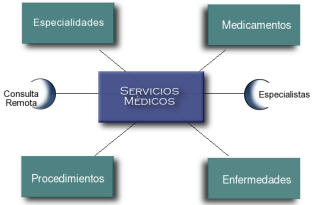
\includegraphics[width=80mm, height=60mm]{servicios.png}
 \caption{Subsistema Servicios Médicos}
 \label{servicios}
\end{figure}

\subsection{Subsistemas Entornos de Aprendizaje} 
Siguiendo la filosofía de integración del SITEM a proyectos de software libre, el subsistema de entornos de aprendizaje incorpora y adapta los elementos de la plataforma \textbf{Moodle} y provee un ambiente en línea para la estructuración, mantenimiento y distribución de conocimiento a través de cursos y seminarios. 

El subsistema permite libre acceso de usuarios a un conjunto de cursos y seminarios que apoyan el desarrollo de competencias en el área de la teleinformática, la telesalud, la telemedicina, las tecnologías de la información y las comunicaciones. Con un enfoque constructivista se procura la retroalimentación de los contenidos por parte de la comunidad. 

Como patrón de desarrollo el SITEM integra a su arquitectura, figura \ref{aplicaciones_sitem}, soluciones exitosas y robustas en el mundo del software libre, de esta forma reutiliza gran cantidad de aplicaciones, las adapta para proveer un ambiente integrado y aumenta sus prestaciones para implementar nuevos casos de uso. Entre las aplicaciones, mostradas en la figura \ref{aplicaciones_sitem}, que contribuyen enormemente en el SITEM se pueden citar:

\begin{description}
 \item[Moodle] Es un ambiente integrado de aplicaciones para la creación, organización, mantenimiento y seguimiento de cursos en línea. El fin primordial de sus herramientas es dar soporte a un marco de educación social constructivista.

\item[PHPBB] Conjunto de módulos escritos en PHP y Python para la gestión de foros en línea; aunque su línea funcional base hace parte de Moodle, en el SITEM los foros de carácter general - aquellos que no pertenecen a un entorno de aprendizaje específico, se implementan usando PHPBB. El manejo de sesiones, la gestión de usuario y la autenticación se han recodificado para que sean compatibles con los subsistemas principales del SITEM.

\item[MediaWiki] Herramienta para la construcción de sitios web tipo Wiki. Un Wiki es un neologismo basado en un término hawaiano y hace referencia a un sitio en el cual el contenido se construye de forma colaborativa usando para ello un lenguaje de etiquetado intermedio que permite la aplicación de cierta plantillas a porciones de texto para poder darles un formato específico. Aunque la información de una página Wiki no esta estructurada, el sistema lleva un historial de cambios por lo que será posible reconstruir el estado de dicha página en cualquier momento de su vida. Este aplicativo esta siendo usado en el SITEM para la construcción de su enciclopedia, los manuales de usuario y en ciertos módulos que requieren la construcción colaborativa de contenidos.

\item[MapServer] Es una aplicación desarrollada en Python que proporciona al SITEM los servicios básicos necesarios para la georeferenciación de la información en el subsistema de consultoría. La plataforma de MapServer define un conjunto de bibliotecas que permiten el manejo de información geográfica. Es software libre y soporta entre otros los formatos: ESRI shapefiles, PostGIS, ESRI ArcSDE, GML; utilizando la librería OGR (http://www.gdal.org/ogr/, 2007).

\item[Google] Su servicio web de motor de búsqueda se usa en el SITEM. Esta es una solución parcial que a corto plazo será desplazada por herramientas de software libre tales como DataparkSearch (http://www.dataparksearch.org/, 2007), ASPSeek (http://www.aspseek.com) y algunas bibliotecas en desarrollo por los integrantes del GITEM.

\item[Sistema de Información Unificado del Sector de Telecomunicaciones] Conocido como SIUST, es un aplicativo Web desarrollado por la Comisión Reguladora de Telecomunicaciones que contiene información del sector de las telecomunicaciones en Colombia: “...información técnica de infraestructura, normatividad del sector, estadísticas comerciales e índices financieros de los prestadores de servicios y los indicadores de gestión del sector entre otros.” \footnote{Tomado del sitio web del SIUST. http://www.siust.gov.co/siust/}

La información, que es de acceso público, permite que el SITEM se nutra de ella para complementar y validar sus propias bases de datos en algunos subsistemas.

\item[Wikipedia] Quizás la fuente de información colaborativa más grande en Internet, debido a que sus contenidos son de uso libre, el SITEM se nutre de ellos y a su vez los complementa. A partir de información disponible se han editado más de 50 artículos en Wikipedia que tienen relación temática con el SITEM.

 \end{description}

\begin{figure}
 \centering
 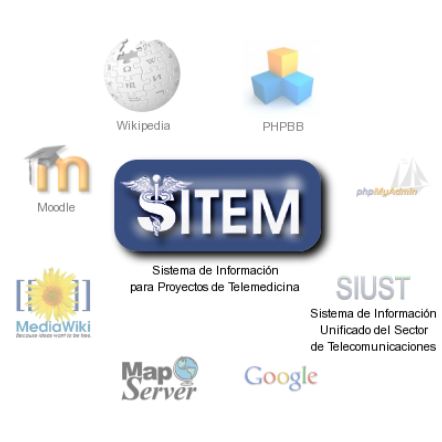
\includegraphics[width=156mm, height=156mm]{sitem_aplicaciones.png}
 \caption{Aplicaciones de Software Libre o Uso libre que complementan al SITEM}
 \label{aplicaciones_sitem}
\end{figure}

Es un objetivo claro del proyecto la integración con otros productos de software libre promoviendo el uso de tales herramientas, el desplazamiento del mercado hacia soluciones basadas en productos de código abierto como estrategia válida para el despliegue de aplicaciones en Telemedicina en entidades que tengan bajos recursos para el montaje y mantenimiento de redes de atención soportas en TIC.

\section {Aspectos Relativos a la Fase de Transición}

El actual despliegue de la solución en una plataforma tecnológica adecuada tal como se muestra en el anexo \ref{modelo_despliegue}, garantiza un óptimo servicio a los potenciales usuarios \footnote{La versión actual esta disponible en Internet en la dirección http://gitem.udistrital.edu.co/sitem/} y marca el paso de la versión 3.0 del producto a la fase de transición. Las herramientas básicas se encuentran disponibles para que el grupo de investigación convoque a las entidades de salud, profesionales en el área de la tecnología, especialistas en medicina y fabricantes - distribuidores - de dispositivos médicos que participaron en la primera fase del Estudio Red de Telemedicina Bogotá \cite{aparicio2000} para que de forma conjunta enriquezcan la base de información en el subproceso de prueba piloto.

Basado en el módulo de generación de herramientas para la recolección de información, anexo \ref{manual_usuario}, el grupo aplicará diferentes instrumentos entre los que se incluyen:

\begin{itemize}
\item Entrevistas: Con el objeto de acordar las directrices a seguir tanto con los operadores de telecomunicaciones, como los prestadores del servicio de salud que participaron de la fase I de recolección de información con el propósito de socializar los resultados del proyecto e invitarlos para que editen y actualicen sus datos obteniendo beneficios incrementalmente. Dichos servicios van desde la disponibilidad de un mapa de sedes, servicios y profesionales hasta la consolidación de información para la gestión de sus redes tecnológicas primarias.

\item Encuestas: Para identificar nuevos requerimientos de servicios que puedan ser desplegados en la plataforma propuesta. Además, estos instrumentos permitirán medir el impacto en la cobertura de los servicios y de participación de las instituciones objeto de la investigación de campo.
\end{itemize}

Las unidades de recolección de información mostradas en el anexo \ref{formulario_preliminar}, se han adaptado de aquellas propuestas por el proyecto europeo HERMES. \footnote{Proyecto de investigación a tres años, financiado por la Comunidad Económica Europea y que cumplió sus objetivos hacia principios del milenio dejando como resultado un conjunto de preguntas básicas que apoyan los procesos de implementación de soluciones médicas apoyadas en las TIC.} El modelo investigación evaluativa que continua en la fase IV del proyecto pretende medir la evolución del nivel de servicios de salud prestados con el apoyo de TIC comparando sucesivamente el modo de operación encontrado entre el año 2000 y 2005 con aquel encontrado entre el año 2008 y 2011 luego que algunas entidades interactúen con el SITEM.

\subsection {Fuentes de Información Primaria}

Para la carga de información inicial en el SITEM se utilizan los resultados del estudio de campo realizado en varias instituciones de carácter público y privado. Dicho resultados se encuentran consignados en sendas tesis en formato digital e impresos disponibles en la biblioteca de la Universidad Distrital y archivo del grupo de investigación:

\begin{itemize}
 \item Hospital Rafael Uribe Uribe.\cite{guarin2003}
 \item Hospital San Pedro Claver.\cite{ardila2001},\cite{rozo2002}
 \item Hospital Simón Bolívar. \cite{acero2002}
 \item Hospital El Tunal. \cite{ruiz2002}\cite{duque2002}
 \item Hospital La Victoria.\cite{barrero2000}
 \item Hospital San José.\cite{gonzalez2002}
\end{itemize}
\chapter{Experiencia de Desarrollo de OpenSITEM}

Como se ha mencionado, openSITEM es centrado en la arquitectura y guiado por casos de uso. Tanto el Director de Proyecto como los equipos de trabajo temporales, están comprometidos con la tarea de generar un aplicativo funcional que esté alineado - de manera emergente, con las vistas arquitectónicas planteadas.

Con el método definido, los artefactos se construyen de manera iterativa e incremental. El ``orden'' en el que aquí se muestra no implica una secuencia de actividades pues no en pocas ocasiones, abordar la disciplina de \textit{Modelado de Dominio} se realiza a continuación de - o en paralelo a, un taller de requisitos y dicho taller surge de una nueva restricción detectada al momento de despliegue. Esta capacidad de adaptación al cambio es lo que ha permitido que openSITEM vaya realizando la transición desde un aplicativo específico a una suite escalable - potenciada por la arquitectura de federación de aplicaciones, orientada a servicios que está implementando.

En la implementación de cada uno de los módulos de openSITEM se siguen las fases contempladas en el Proceso Unificado\footnote{Inicio, elaboración, construcción y transición.} y se desarrollan flujos de trabajo en las disciplinas básicas de:

\begin{itemize}
\item Requisitos.
\item Arquitectura.
\item Elaboración.
\item Pruebas.
\item Despliegue.
\end{itemize}

A partir de iteraciones continuas por las diferentes disciplinas se refinan constantemente los modelos y se presentan resultados que permiten medir los avances, así como comprobar los niveles de calidad y la validez tanto de los entregables como del método empleado. 

\section{Modelo de Requisitos}

Un requisito es una declaración explícita y aceptada de la funcionalidad que un usuario espera del sistema. Dicha declaración debe ser coherente con el objeto de estudio de openSITEM, respetando siempre los principios normativos y de propiedad intelectual. Cada requisito se plasma en un documento denominado Caso de Uso, el cual describe un conjunto de escenarios de interacción del usuario con el sistema, con el propósito de obtener algo de valor.

\subsection{Declaración del Problema}

OpenSITEM es una propuesta de solución a los siguientes problemas:

\begin{itemize}
 \item La información de los estudios de campo no está estructurada, está dispersa, se ha perdido y es difícil de consultar y consolidar.
 \item El equipo de diseño de GITEM no cuenta con un mecanismo estándar para caracterizar los componentes de las redes de eSalud.
 \item No es posible determinar el valor de un nodo dentro de una red de eSalud.
 \item No existe capacidad de análisis multitemporal para determinar la valides de la categorización de nodos de una red de eSalud.
\end{itemize}

\subsection{Responsabilidades del Sistema}

El sistema debe contribuir a que los investigadores:

\begin{itemize}

\item Caractericen nodos con potencialidad de pertenecer a redes de eSalud.
\item Creen instancias de nodos a partir de la información de los estudios de campo que desarrollo el grupo.
\item Comparen nodos de la misma categoría para definir cual tiene mayor valor relativo.
\item Consulten catálogos especializados en cada categoría de nodos.
\item Definan modelos de categorías de nodos.
\item Evalúen la potencialidad de un nodo para pertenecer a una red de eSalud.
\end{itemize}


\section{Alcance}

OpenSITEM no implementa todo el modelo del requisitos. Los módulos desarrollados son prototipos funcionales que sirven de guía para el desarrollo y evolución posterior de la solución. Si relacionamos esto con el proceso OpenUP, el grupo en la fase III alcanza el final de la fase elaboración.

\section{Definición de actores}

El sistema es manejado por varios tipos de usuarios, cada uno con características específicas. Este tratamiento especial tiene que ver con el mantenimiento de la integridad de la información, la cual solo puede ser gestionada por un grupo selecto de usuarios. 

Algunos actores esperados en el openSITEM son:

\begin{itemize}
\item Administrador.
\item Consultor.
\item Especialista Médico.
\item Profesional TIC.
\item Usuario General.
\end{itemize}

Cada uno de ellos con las características mostradas en el anexo \ref{modelo_requisitos}.

\section{Casos de uso}

Los requisitos funcionales son declarados con diferente nivel de detalle empleando casos de uso, diagramas de comportamiento y de interacción. Al caracterizar una interacción por medio de un caso de uso se espera tener información acerca de:

\begin{itemize}
\item Nombre del Caso de Uso
\item Objetivo que se logra al ejecutarse el caso de uso.
\item Código que lo identifique unívocamente dentro del banco de artefactos.
\item Actores que intervienen al desarrollarse el caso de uso.
\item Casos de uso con los que está relacionado.
\item Precondiciones.  El estado del sistema que debe asegurarse antes de que el caso de uso inicie. Debido a que es responsabilidad del sistema no se verifica en el caso de uso.
\item Postcondiciones. Las características y estado del sistema una vez se haya terminado el caso de uso.
\item Flujo de Tareas. Flujo principal y flujos alternativos de las actividades que se suceden para lograr la funcionalidad deseada. Se debe mantener claridad en el modelo por lo que se recomienda utilizar diferentes artefactos para los flujos alternativos cuando esto lo amerite.
\end{itemize}

La tabla \ref{casouso}, muestra el flujo principal del un caso de uso de openSITEM.

\begin{table}
\begin{center}
\begin{tabular}{|l|p{10cm}|}
\hline
\textbf{Caso de Uso}&\\
\hline
Nombre & Evaluar Capacidad de un Nodo\\
\hline
Objetivo & El actor asigna un valor y un diagnóstico a un nodo que da cuenta de la capacidad que tiene dicho nodo de pertenecer a una red de eSalud .\\
\hline
Código Interno & UC-GENERAL-XXXX \\
\hline
Actores & Consultor\\
\hline
Precondiciones & El nodo se encuentra registrado en el sistema en estado ACTIVO.\\
\hline
Flujo Básico & 1. El Consultor selecciona el nodo que desea evaluar.\\
& 2. OpenSITEM presenta los datos relacionados con el nodo\\
& 3. El Consultor revisa el historial de valoraciones del nodo.\\
& 4. El Consultor revisa el valor de los atributos del nodo. \\
& 5. El Consultor valora el nodo.\\
& 6. El Consultor argumenta la valoración a través de un diagnóstico.\\
& 7. OpenSITEM guarda los datos de la valoración.\\
& 8. OpenSITEM envía una notificación de la valoración a los interesados.\\
\hline
Postcondiciones & Se agregó una valoración argumentada al sistema.\\
\hline
Casos de uso relacionados&Consultar Historial de Valoración de Nodo\\
\hline
\end{tabular}
\caption{Caso de Uso Evaluar Capacidad de Nodo}
\label{casouso} 
\end{center}
\end{table}

El modelo actual tiene 80 casos de uso principales definidos\footnote{No se incluyen casos de uso implementados en aplicaciones conexas.} y más de 230 flujos alternativos - los más relevantes incluidos en el anexo \ref{modelo_requisitos}. Con esto se concreta los requerimientos de más alto nivel definido por el grupo GITEM. Se recalca que el grueso de ellos aún no se han desarrollado por lo que se probablemente el modelo se adapte a medida que se progresa en la construcción.

\section{Arquitectura}

Los requisitos son insumo para modelar los elementos del sistema y sus relaciones. El equipo de desarrollo se ha apoyado en diferentes diagramas de estructura y de comportamiento e interacción para describir la estructura y el comportamiento del sistema. El anexo \ref{modelo_analisis} corresponde a las vistas de la arquitectura que contienen los elementos más interesantes para diferentes partes del sistema. Como puede observarse en dicho anexo, se han aplicado varios patrones de diseño \footnote{Basados en General Responsibility Assignment Software Patterns (GRASP) y GoF} \cite{larman2003}, \cite{gamma1994} especialmente se presta atención a mantener los principios de:

\begin{itemize}
\item Alta Cohesión
\item Bajo Acoplamiento
\end{itemize}

Asignando responsabilidades teniendo en cuenta:
\begin{itemize}
\item Experto en Información.
\item Controlador
\end{itemize}

En la figura \ref{secuencia}, se muestra el diagrama de interacción correspondiente a la realización del caso de uso no esencial de registrarse en el sistema.

\begin{figure}
 \centering
 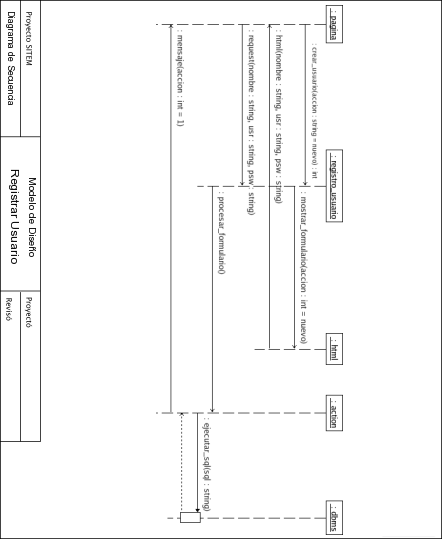
\includegraphics[width=156mm, height=156mm]{secuencia.png}
 \caption{Realización del Caso de Uso registrarse en el Sistema}
 \label{secuencia}
\end{figure}


\section{Modelo de Implementación}

El conjunto de diagramas del Anexo \ref{modelo_analisis} brinda la información fundamental para el modelo de implementación. En el openSITEM se agrupan los diferentes componentes en la jerarquía de carpetas mostrada en la figura \ref{carpetas_sitem}.

Cada una de las carpetas contiene los ficheros de código fuente del producto:

\begin{itemize}
 \item \textbf{Clases:} Contiene los archivos en PHP que implementan las clases. 
\item \textbf{Funciones:} Grupo de funciones en JavaScript para la validación de información en el nodo de usuario. En la actualidad la fase IV contempla complementar esta aproximación con la utilización de AJAX.
\item \textbf{Configuración:} Alberga el archivo \textit{config.inc.php} que guarda las variables de ingreso a la base de datos. Dichas variables se encuentran codificadas de acuerdo al algoritmo que se seleccione (o implemente) desde la clase \textit{codificar}.
\item \textbf{Bloques:} Agrupa el código fuente de cada bloque desarrollado en el openSITEM. Un bloque se define como una unidad de funcionalidad independiente que puede utilizarse en cualquier página.
\item \textbf{Estilo:} Información acerca de los parámetros generales de estilo - tamaño de fuente, color de bordes, fondos, colores de letras, etc; para diferentes componentes del openSITEM. La modificación o inclusión de parámetros afectará la interfaz global del sistema. Actualmente los estilos en el openSITEM se basan en hojas de estilo CSS.
\item \textbf{Gráficos:} Todos los archivos gráficos usados en el proyecto.
\item \textbf{Documentos:} Carpeta inicialmente vacía que se utiliza para guardar los archivos que los usuarios carguen a través del protocolo HTTP. Por seguridad se recomienda que esta carpeta se encuentre fuera del directorio en donde se encuentra instalada la aplicación.
\item \textbf{Instalar:} Contiene el instalador del producto. Esta carpeta debería ser retirada una vez el sitio se encuentre en producción.
\item \textbf{Desarrollo:} Con varios scripts que facilitan la tarea de desarrollo y adaptación de bloques en el sistema. Estos scripts se han construidos pensando en plataformas de desarrollo y prueba por lo que se supone no debe encontrarse en plataformas de producción.
\end{itemize}

En todo caso, durante el proceso de instalación se puede - y recomienda; asociar nuevos nombres a las carpetas por lo que en teoría ningún desarrollo basado en el openSITEM que esté en etapa de producción debería tener nombres de carpetas conocidos.

\begin{figure}
 \centering
 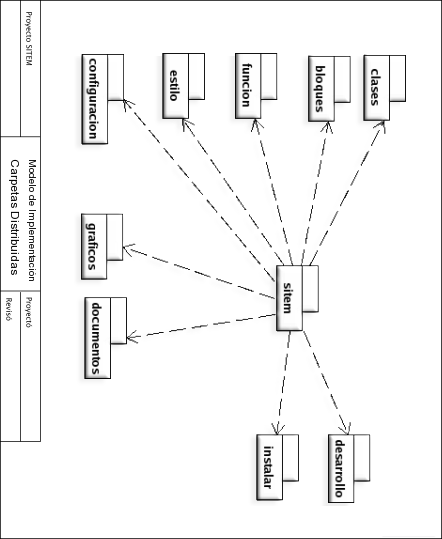
\includegraphics[width=156mm, height=156mm]{carpetas.png}
 \caption{Carpetas que se distribuyen con el openSITEM}
 \label{carpetas_sitem}
\end{figure}

\section{Acerca de la Seguridad en el Sistema}

Al tratarse de una aplicación web se tiene grandes retos con la seguridad. Se emplea como referencia el top 10 del proyecto OWASP\cite{owasp2017}, que para el año 2017 considera que los riesgos más importantes son: 

\begin{itemize}
  \item Inyección.
  \item Fallos en la Autenticación.
  \item Exposición de datos sensibles.
  \item Entidades externas XML.
  \item Fallos en el Control de Acceso.
  \item Fallos en la configuración.
  \item Cross-Site Scripting (XSS).
  \item De-serialización insegura.
  \item Uso de componentes con vulnerabilidades conocidas.
  \item Gestión y seguimiento ineficiente a los registros del sistema.
\end{itemize}

Para cada una de estos riesgos el equipo de desarrollo ha estudiado e implementado las técnicas y controles que la misma guía de la OWASP declara. La documentación del modelo de seguridad está siendo elaborada en el marco de una tesis de pregrado, la cual se encuentra en sus primeras etapas.

Como ejemplo, la figura\ref{desenlace} muestra la manera que OpenSITEM implementa un control sobre A2:2017, usando el gestor de sesiones de lado de servidor para generar un identificador aleatorio para cada una de las peticiones de página. Dicha técnica se asegura de crear cada cierto periodo de tiempo\footnote{Predefinido a 5 minutos} una llave única que garantiza un alto nivel de entropía en la cadena codificada - lo que implica que cada recurso tendrá un tiempo de expiración.

\begin{figure}
 \centering
 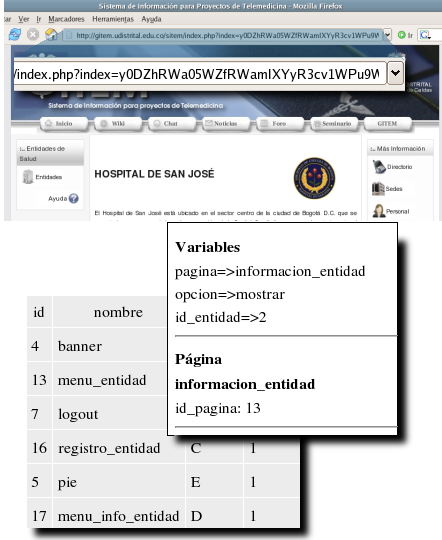
\includegraphics[width=80mm]{desenlace.png}
 \caption{URL encriptada. Con la herramienta \textit{Desenlace} el desarrollador puede descifrar los datos}
 \label{desenlace}
\end{figure}

En cuanto a la integridad de los datos se tiene un modelo de comparación de contenidos que se activa cada periodo de tiempo, el cual es programable; proponiéndose mantener una copia de respaldo verificada y avalada por el administrador. En caso de corrupción o pérdida de datos se mantiene una lista completa de los usuarios del sistema de hasta 1’000.000 de sesiones de tipo desplazamiento en donde el usuario más antiguo es descartado para la inclusión del nuevo cuando el tamaño asignado es completado, asegurándose el manejo eficiente de disco. 

Por ningún motivo se permite el acceso a sitios restringidos a usuarios que no hayan sido plenamente identificados en el sistema. En sitios críticos se hace una revisión de los datos de acceso guardados en cookies o se constata los datos de inicio de sesión. Se han evitado al máximo el uso de carácter comodín y todos los accesos a la base de datos son validados en su sintaxis. El openSITEM actualmente propone el uso de protocolos seguros tales como SSL.

Vale la pena destacar el uso de métodos de autenticación de usuario basado en sesiones y codificación de datos que permiten ofrecer un contenido personalizado de acuerdo al perfil de cada uno de los clientes del sistema.


\section{Modelo de Datos}

Dentro del proceso de desarrollo del openSITEM el modelado y elaboración del sistema de bases de datos es una de las partes fundamentales de la propuesta. Se ha venido estructurando el modelo de acuerdo a las necesidades de cada módulo en particular para garantizar la independencia entre ellos en cada una de las capas, incluyendo la de persistencia.

Dependiendo de las características de cada subsistemas se implementan o no políticas transaccionales. El modelo de seguridad en los datos hereda todos los elementos del servidor tales como bloqueos de puertos, ocultación de ventanas, manejo de sockets, etc; además, un esquema lógico de validación por conexiones persistentes complementa estas características.

El anexo \ref{modelo_datos} contiene los diagramas de clases que describen la arquitectura de datos del sistema y cada uno de sus subsistemas asociados. 

En la actualidad el openSITEM acepta bases de datos PostgreSQL, MySQL y ORACLE. La capa de persistencia del hilo principal se despliega sobre un servidor MySQL.


\section{Interfaz gráfica.}

De acuerdo a los diagramas conceptuales del portal GITEM y de openSITEM. Se han utilizado para la creación de las páginas los conceptos de diseño web enumerado por \cite{krug2014}, intentando evitar al máximo las páginas sobrecargadas de información. La navegación es guiada mediante enlaces, los cuales están agrupados temáticamente logrando una coherencia en el contenido. 

Los gráficos han sido optimizados y su inclusión es necesaria para dar ayuda visual al contenido basado en texto. Teniendo en cuenta que el openSITEM esta diseñado para interactuar permanentemente y por periodos prolongados de tiempo con el cliente, se han evitado deliberadamente la utilización  de componentes dinámicos. No obstante, el diseño no pierde atractivo ya que su implementación se fundamenta en bibliotecas de uso extendido.

Para reducir el tiempo de acceso al portal, sobre todo cuando se trabaja con conexiones lentas, se da la posibilidad en algunos subsistemas de descargar en formato PDF todo el contenido del grupo de páginas en donde se este ubicado.

\subsection{Arquitectura de la página}

Independiente del subsistema que nos encontremos las páginas siempre están compuestas por cinco secciones denominadas genéricamente con las letras A, B, C, D y E. En ellas se distribuyen los diferentes bloque que conforman la página en una arquitectura Top - Down. Las páginas que no tienen bloques en todas las secciones colapsan aquellas que no se utilizan para dar una impresión visual consistente. Las figuras \ref{secciones} y \ref{seccion_colapsada} muestran gráficamente el manejo de las secciones en cada página.

\begin{figure}
 \centering
 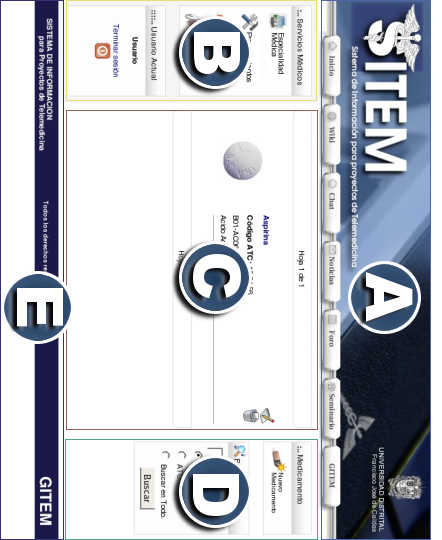
\includegraphics[width=156mm, height=156mm]{secciones.png}
 \caption{Arquitectura de una página en el openSITEM}
 \label{secciones}
\end{figure}

\begin{figure}
 \centering
 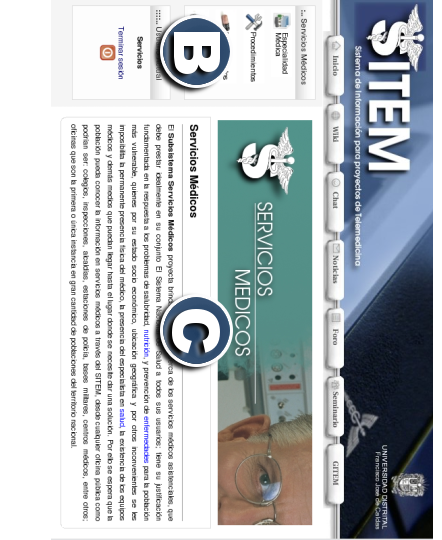
\includegraphics[width=156mm, height=156mm]{seccion_colapsada.png}
 \caption{Página del openSITEM en donde la Sección D se ha colapsado.}
 \label{seccion_colapsada}
\end{figure}

\section{Entregables del proyecto}

Los siguientes artefactos – documentos, son generados y utilizados por el proyecto. En el anexo \ref{entregables} se tiene extractos importantes de algunos de ellos.

\begin{itemize}
\item \textbf{Plan General de Trabajo}
\item \textbf{Modelo de Casos de Uso}. El cual especifica los requerimientos que debe cumplir el módulo de software y que en últimas constituye los contratos que éste, el módulo, tiene con actores externos. Este artefacto estará hecho en su totalidad usando el Lenguaje de Modelado Unificado. 

Dentro de este modelo se tienen dos vistas claras: la del negocio y la del sistema. El modelo de Casos de Uso del Negocio ilustra el ámbito del negocio que esta siendo modelado. El diagrama contiene actores del negocio y los servicio o funciones que ellos requieren del negocio. El modelo de casos de uso del sistema representa el ámbito de una aplicación. De esto se tiene que un solo modelo de casos de uso del negocio puede tener muchos Modelos de casos de uso asociados, donde cada modelo de casos de uso representa una única aplicación.

\item \textbf{Modelo de Objetos.} El cual describe la forma en que cada requerimiento – o contrato,  es cumplido. Establece las entidades internas, la información que intercambian y los flujos de trabajo que logran el cumplimiento de los requisitos. Los grafos correspondientes podrán incluir diagramas estáticos o interactivos expresados en UML.

\item \textbf{Glosario.} Que es el único artefacto válido de consulta para la terminología usada en el desarrollo del openSITEM. Ver el anexo \ref{glosario}.

\item \textbf{Visión.} Este documento define la visión del openSITEM. Es de todos el que marca las pautas conceptuales. 

\item \textbf{Especificaciones Adicionales.} Este documento captura los requisitos que no han sido incluidos como parte de los casos de uso y se refieren requisitos no-funcionales globales. Dichos requisitos incluyen: requisitos legales o normas, aplicación de estándares, requisitos de calidad del producto, tales como: confiabilidad, desempeño, etc., u otros requisitos de ambiente, tales como: sistema operativo, requisitos de compatibilidad, etc. 

\item \textbf{Prototipos de Interfaces de Usuario.} Se trata de prototipos que permiten al usuario hacerse una idea más o menos precisa de las interfaces que proveerá el sistema y así, conseguir retroalimentación de su parte respecto a los requisitos del sistema. Estos prototipos se realizarán como: dibujos a mano en papel, dibujos con alguna herramienta gráfica o prototipos ejecutables interactivos, siguiendo ese orden de acuerdo al avance del proyecto. Sólo los de este último tipo serán entregados al final de la fase de Elaboración, los otros serán desechados. Asimismo, este artefacto, será desechado en la fase de Construcción en la medida que el resultado de las iteraciones vayan desarrollando el producto final. 

\item \textbf{Arquitectura.} Este modelo establece la realización de los casos de uso en clases y pasando desde una representación en términos de análisis (sin incluir aspectos de implementación) hacia una de diseño (incluyendo una orientación hacia el entorno de implementación), de acuerdo al avance del proyecto.  Consultar el anexo \ref{modelo_analisis}.

\item \textbf{Modelo de Datos.} Previendo que la persistencia de la información del sistema será soportada por una base de datos relacional, este modelo describe la representación lógica de los datos persistentes, de acuerdo con el enfoque para modelado relacional de datos. Para expresar este modelo se utiliza un Diagrama de Clases (donde se utiliza un profile UML para Modelado de Datos, para conseguir la representación de tablas, claves, etc.). El anexo \ref{modelo_datos} contiene los artefactos más importantes del modelo de datos. 

\item \textbf{Modelo de Implementación.} Este modelo es una colección de componentes y los subsistemas que los contienen. Estos componentes incluyen: ficheros ejecutables, ficheros de código fuente, y todo otro tipo de ficheros necesarios para la implantación y despliegue del sistema.

\item \textbf{Modelo de Despliegue.} Este modelo muestra el despliegue la configuración de tipos de nodos del sistema, en los cuales se hará el despliegue de los componentes. Ver anexo \ref{modelo_despliegue} 

\item \textbf{Casos de Prueba.} Cada prueba es especificada mediante un documento que establece las condiciones de ejecución, las entradas de la prueba, y los resultados esperados. Estos casos de prueba son aplicados como pruebas de regresión en cada iteración. Cada caso de prueba llevará asociado un procedimiento de prueba con las instrucciones para realizar la prueba, y dependiendo del tipo de prueba dicho procedimiento podrá ser automatizable mediante un script de prueba. 

\item \textbf{Solicitud de Cambio.} Los cambios propuestos para los artefactos se formalizan mediante este documento. Mediante este documento se hace un seguimiento de los defectos detectados, solicitud de mejoras o cambios en los requisitos del producto. Así se provee un registro de decisiones de cambios, de su evaluación e impacto, y se asegura que éstos sean conocidos por el equipo de desarrollo. Los cambios se establecen respecto de la última baseline (el estado del conjunto de los artefactos en un momento determinado del proyecto) establecida. En nuestro caso al final de cada iteración se establecerá una baseline. 

\item \textbf{Plan de Iteración.} El conjunto de actividades y tareas se orden temporalmente y se le asignan recursos a corto plazo. Se realiza para cada iteración y en todas las fases. 

\item \textbf{Lista de Riesgos.} Este documento incluye una lista de los riesgos conocidos y vigentes en el proyecto, ordenados en orden decreciente de importancia y con acciones específicas de contingencia o para su mitigación. El anexo \ref{riesgos} contiene la declaración de los riesgos más importantes detectados en el proyecto así como estrategias para minimizarlos.

\end{itemize}
\begin{thebibliography}{}

\bibitem[Acero y Ariza,2002] {acero2002} Acero, D. Ariza, M.\textit{Requerimientos tecnicos y financieros para la implementacion de una red piloto de Telemedicina en el Hospital Simón Bolivar}.Grupo de Investigación en Telemedicina,  Universidad Distrital Francisco José de Caldas.2002.

\bibitem[Alhir,2003] {alhir2003} \textit{Understanding the Unified Process.} Methods and Tools, Martinig Associates. 2002.

\bibitem[Aparicio-Ramirez,2003] {aparicio2003} Aparicio,L. y Ramírez, J.\textit{Arquitectura de Red de Telemedicina}, Centro de Investigaciones y Desarrollo Científico, Universidad Distrital F.J.C, 2003.

\bibitem[Aparicio,2000] {aparicio2000} Aparicio,L.\textit{Propuesta de Estudio Red de Telemedicina Bogota}, Grupo GITEM, Universidad Distrital F.J.C, 2000.

\bibitem[Ardila,2001] {ardila2001} Ardila,J y Ardila, M.\textit{Evaluación y diagnóstico de los servicios básicos y especializados al servicio de la salud de la clínica San Pedro Claver para el desarrollo de la red de Telemedicina de Bogotá}.Grupo de Investigación en Telemedicina,  Universidad Distrital Francisco José de Caldas.2001.


\bibitem[Bashshur,1977] {bashshur77} Bashshur, R., Lovett J. \textit{Assessment of telemedicine: results of the initial experience.} Aviation, Space and Environmental Medicine 1977.

\bibitem[Bashshur,1995] {bashshur95} Bashshur, R. \textit{On the Definition and Evaluation of Telemedicine. Telemedicine Journal.} Volume 1, Number 1, Mary Ann Liebert, Inc., Publishers. 1995.

\bibitem[Beck,1999] {beck1999} Beck, K. \textit{ Extreme Programming Explained: Embrace Change }. Addison-Wesley. 1999.

\bibitem[Benafia,2016] {benafia2016} Benafia, A., Mazouzi, S. y Maanru, R. \textit{From Linguistic to Conceptual: A Framework Based on a Pipeline for Building Ontologies from Texts}. Journal of Advanced Computational Intelligence and Intelligent Informatics. 2016.

\bibitem[Bergeron,2003] {bergeron2003} Bergeron, B. \textit{Essentials of knowledge management.} Jhon Wiley \& Sons, New Jersey, 2003.

\bibitem[Bos,2004] {bos2004} Bos,B.\textit{A proposal for Webapps}. W3C Consortium,2004.

\bibitem[Boggs,2002] {boggs2002} Boggs,W. Boogs, M.\textit{UML with Rational Rose 2002}. SyBex,2002.

\bibitem[BCE,2003] {bce} Britannica Concise Encyclopedia.\textit{Anarchism.}. Obtenido en julio 18, 2003, desde:    http://search.eb.com/ebc/article?eu=380585.

\bibitem[Brugge, Dutoit, 2000] {objectoriented} Brugge, B. y Dutoit, A.~H.\textit{Object-Oriented Software Engineering}. Prentice Hall, 2000.

\bibitem[McCarty, 2006] {carty} Carty, J. \textit{Dynamics of Software Development}.Microsoft Press, 2006.

\bibitem[Cockburn, 1999] {cockburn1999} Cockburn, A. \textit{The Impact of Object-Orientation on Application Development.} IBM Systems Journal 38. Páginas 308-332, 1999.

\bibitem[Ley 23,1982] {congreso23} Congreso de la República. \textit{Ley 23 de 1982: Sobre Derechos de Autor}. República de Colombia, 1982.

\bibitem[Dec 1360,1989] {congreso1360} Congreso de la República. \textit{Decreto 1360 de 1989: Inscripción del soporte lógico (software) en el Registro Nacional del Derecho de Autor}. República de Colombia, 1989.

\bibitem[Ley 44,1993] {congreso44} Congreso de la República. \textit{Ley 44 de 1993: Modifica y adiciona la Ley 23 de 1982 y modifica la Ley 29 de 1944}. República de Colombia, 1993.

\bibitem[Ley 565,2000] {congreso565} Congreso de la República. \textit{Ley 565 de 2000: adopción del Tratado de la OMPI sobre Derechos de Autor}. República de Colombia, 2000.

\bibitem[CRT,QoS,2006] {crtcondiciones} Comisión de Regulación de Telecomunicaciones. \textit{Condiciones de Calidad en Servicios de Telecomunicaciones.} República de Colombia, 2006. 

\bibitem[CRT,Indicadores,2006] {crtindicadores} Comisión de Regulación de Telecomunicaciones. \textit{Indicadores de Calidad en Servicios de Telecomunicaciones.} República de Colombia, 2006. 

\bibitem[CRT,QoS,2007] {crtqos} Comisión de Regulación de Telecomunicaciones.\textit{Proyecto de Resolución para Indicadores de Calidad de Servicio.} República de Colombia, 2007.

\bibitem[Corte1319,2001] {sentencia1319} Corte Constitucional de Colombia.\textit{Sentencia T-1319 de 2001.} República de Colombia, 2001

\bibitem[Craig, 2005] {craig2005} Craig J, Patterson V. \textit{Introduction to the practice of telemedicine.} Journal of Telemedicine and Telecare. 2005. Págs 3-9.

\bibitem[Davenport,1998] {davenport1998} Davenport, T. y Prusak, L.\textit{Working Knowledge: How Organizations Manage What They Know}, Harvard Business School Press, Boston.1998

\bibitem[Davies,2011] {davies2011}. Davies, M. Knowledge – Explicit, implicit and tacit: Philosophical aspects. , International Encyclopedia of Social and Behavioral Sciences, Elsevier. 2011.

\bibitem[Dueck,2001] {dueck2001} Dueck,G.\textit{Views of knowledge are human views.}IBM Systems Journal, Volumen 40, Número 4, 2001.

\bibitem[Duque \textit{et al},2002] {duque2002} Duque,J. García J, Caicedo, D.\textit{Estudio sobre los requerimientos técnicos y financieros para implementar los servicios telemédicos en el Hospital El Tunal,  para el proyecto telemedicina Bogotá 2000.}.Grupo de Investigación en Telemedicina,  Universidad Distrital Francisco José de Caldas.2002.

\bibitem[UN, 2005] {egovernment} Department of Economic and Social Affairs.\textit{UN Global E-government Readiness Report 2005 From e-government to e-inclusion}. Naciones Unidas, New York, 2005.

\bibitem[Firestone,2001] {firestone2001} Firestone, J.\textit{Key Issues in Knowledge Management. Knowledge and Innovation.} Knowledge Management Consortium International. Volumen 1. 2001.

\bibitem[Gang,2007] {gang2007} Gang, L. y Yi, L. \textit{A Relational Model of Knowledge Share, Knowledge Acquisition and Product Innovation}. Universidad Xi'an Jiaotong. China. 2007.

\bibitem[Girard,2015] {girard2015} Girard, J. \textit{Defining knowledge management: Toward an applied compendium}. Online Journal of Applied Knowledge Management. International Institute for Applied Knowledge Management. 2015.

\bibitem[González y Torres,2002] {gonzalez2002} González, O. Torres, J.\textit{Evaluación y Diagnóstico de los Servicios Básicos y Especializados al Servicio de la Salud del Hospital de San José para el Desarrollo de la Red de Telemedicina de Bogotá.} Grupo de Investigación en Telemedicina, Universidad Distrital Francisco José de Caldas.2002.

\bibitem[Guarin \textit{et al},2003] {guarin2003} Guarin, S. Garcia, M. Torres, L.\textit{Diagnóstico de las Redes Eléctrica, Telefónica y de Datos del Hospital Rafael Uribe Uribe E.S.E.} Grupo de Investigación en Telemedicina,  Universidad Distrital Francisco José de Caldas.2003.

\bibitem[Hurtado,2000] {hurtado2000} Hurtado,J.\textit{Metodología de la Investigación Holística.} Sypal, Caracas, Venezuela, 2000.

\bibitem[Hibbard,1997] {hibbard1997} Hibbard, J. \textit{Knowledge management—knowing what we know.} Information Week, Edición Octubre de 1997.

\bibitem[IEEE, 1990] {softwareengineering} IEEE Institute.\textit{IEEE Standard Glossary of Software Engineering Terminology - IEEE std 610.12-1990}. IEEE, 1990.

\bibitem[Koch, 2005] {koch} Koch, S. \textit{Free Open Source Software Development}. Idea Group, 2005.

\bibitem[Liebowitz,1998] {liebowitz1998} Liebowitz, J. y Beckman, T. \textit{Knowledge Organizations: What Every Manager Should Know}. Boca Raton, St. Luci press, 1998.

\bibitem[ITU-T, 2004] {ITU2004} ITU-T. \textit{Manual Calidad de servicio y calidad de funcionamiento de la red}. Unión Internacional de Telecomunicaciones, 2004.

\bibitem[ITU-OMS, 2012] {ituoms2012} ITU - OMS. \textit{National eHealth Strategy Toolkit}. Unión Internacional de Telecomunicaciones. 2012 


\bibitem[G1000, 2001] {ITUG1000} ITU-T. \textit{Recomendación G.1000 - Calidad de servicio en las comunicaciones: Marco y definiciones}. Unión Internacional de Telecomunicaciones, 2001.

\bibitem[G1010, 2001] {ITUG1010} ITU-T. \textit{Recomendación G.1010 - Categorías de calidad de servicio para los usuarios de extremo de servicios multimedios}. Unión Internacional de Telecomunicaciones, 2001.

\bibitem[Jacobson,2000] {jacobson2000} Jacobson,I. Booch,G y Rumbaugh,J. \textit{El Proceso Unificado de Desarrollo de Software}. Addison-Wesley, Madrid, 2000.

\bibitem[Jacobson,2005] {jacobson2005} Jacobson,I. Booch,G y Rumbaugh,J. \textit{The Unified Modeling Language Reference Manual}, segunda edición. Addison-Wesley, Boston, 2005.

\bibitem[Jackson,2005] {jackson2005} Jackson,D.\textit{The W3C Workshop on Web Applications and Compound Documents}. W3C Consortium,2005.

\bibitem[Larman,2004] {larman2004} Larman,C. \textit{Agile and iterative development: a manager ’s guide.} Addison Wesley, 2004.

\bibitem[Larman,2003] {larman2003} Larman, C. \textit{UML y PATRONES. Una introducción al análisis y diseño orientado a objetos y al Proceso Unificado}. Pearson Educación S.A. Madrid, 2003.

\bibitem[Martínez,1998] {martinez1998} Martínez, R. Martín, F. \textit{LANDSCAPE: A Knowledge-Based System for Visual Landscape Assessment.}. IEA/AIE, Volumen 2. Springer, 1998. Páginas 849-856.

\bibitem[CONPES3072,2000] {mincomunicaciones3072} Ministerio de Comunicaciones.\textit{Documento CONPES 3072 - Agenda de Conectividad}. República de Colombia, 2000.

\bibitem[MINSALUD-4678,2015] {minsalud4678} Ministerio de Salud.\textit{Resolución Número 4678 de 2015}. República de Colombia, 2015.

\bibitem[MINSALUD-1448,2006] {minsalud1448} Ministerio de Salud.\textit{Resolución Número 1448 de 2006}. República de Colombia, 2006.

\bibitem[Barrero,2000] {barrero2000} Muñoz, F. Barrero, J.\textit{Evaluación y Diagnóstico de los Servicios Básicos y Especializados al Servicio de la Salud del Hospital La Victoria para el Desarrollo de la Red de Telemedicina de Bogotá}. Grupo de Investigación en Telemedicina,  Universidad Distrital Francisco José de Caldas.2000.

\bibitem[Nokata,1994] {nokata1994} Nonaka, I.\textit{A dynamic theory of organizational knowledge creation.} Organization Science,5,1994. pp. 14-37.

\bibitem[Nokata,1995] {nokata1995} Nonaka,I. y Takeuchi, H.\textit{The Knowledge Creating Company: How Japanese Companies Create the Dynamics of Innovation.} Oxford University Press,1995.

\bibitem[OMG, 2007] {omg2007} OMG.\textit{Unified Modeling Language: Specification. Versión 2.1.1}. Object Management Group, 2007.

\bibitem[OMG, 2007a] {omg2007a} OMG.\textit{Unified Modeling Language: Superstructure. Versión 2.1.1}. Object Management Group, 2007.

\bibitem[OMS, 2010] {oms2010} Organización Mundial de la salud. \textit{Telemedicine: opportunities and developments in Member States: report on the second global survey on eHealth 2009}. 2010

\bibitem[OMS, 2016] {oms2016} Organización Mundial de la salud. \textit{Global difusion of eHealth: making universal health coverage achievable. Report of the third global survey on eHealth}. 2016

\bibitem[OPS, 2011]{ops2011}. Organización Panamericana de la Salud. \textit{Estrategia y Plan de Acción sobre eSalud}. 51 Consejo Directivo, 2011

\bibitem[Pressman, 2006] {pressman} Pressman, R.~J.\textit{Ingeniería del Software}. Sexta Edición. Mc Graw 
Hill, México, 2006.

\bibitem[Raymond, 1996] {raymond} Raymond,E.\textit{The Cathedral and the Bazaar}, Revision 1.57, 2000.

\bibitem[AIM,1993] {aim} \textit{Research and technology development on telematics systems in health care: AIM 1993; Annual Technical Report on RTD: Health Care.} Comisión Europea: Dirección General XIII, 1993.

\bibitem[Rozo \textit{et al},2002] {rozo2002} Rozo, O. Valencia, S. Barahona, F.\textit{Estudio diagnóstico de las condiciones técnicas y financieras en instrumentos y equipos médicos  y de servicios de la clínica San Pedro Claver para la implentación de los servicios telemédicos.} Grupo de Investigación en Telemedicina,  Universidad Distrital Francisco José de Caldas.2003.

\bibitem[Ruiz y Niño,2002] {ruiz2002} Ruiz, M. Niño, D.\textit{Evaluacion y Diagnostico de los Servicios Basicos y Especializados al Servicio de la Salud del Hospital El Tunal para el Desarrollo de la Red de Telemedicina de Bogotá} Grupo de Investigación en Telemedicina,  Universidad Distrital Francisco José de Caldas.2002.

\bibitem[Salazar,2002] {oas2002} Salazár,J. y Kopec, A.\textit{Aplicaciones de Telecomunicaciones en Salud en la Subregion Andina - Telemedicina}, Organismo Andino de Salud, OPS. 2002.

\bibitem[Sarmento,2005] {sarmento2005} Sarmento,A.\textit{Issues of human computer interaction}.IRM Press, Londres, 2005. 

\bibitem[Sowa,1984] {sowa1984} Sowa, J. \textit{Conceptual Structures: Information Processing in Mind and Machine.} Addison-Wesley,1984.

\bibitem[stallman,2002] {stallman2002} Stallman,R.\textit{Free Software, Free Society:Selected Essays of Richard M. Stallman}. GNU Press, Bosotón, 2002.

\bibitem[Tatnall, 2003] {tatnall2005} Tatnall,A. \textit{Web portals:The New Gateways to Internet Information and Services.} Idea Group, Londres, 2005.

\bibitem[BDT,1999] {itu} \textit{Telemedicine And Developing Countries - Lessons Learned}. Document 2/116-E. ITU-D STUDY GROUPS. Question 14/2: Fostering the application of telecommunication in health care.  Identifying and documenting success factors for implementing telemedicine. 1999.

\bibitem[Bangemann,1994] {bangeman} \textit{The Bangemann Report: Europe and the global Information Society. Recomendaciones al Consejo Europeo.} Bruselas, 1994. Disponible en http://www.cordis.lu.

\bibitem[Turban,1992] {turban1992} Turban, E.\textit{Decision Support and Expert Systems - Management Support Systems.} Collier Macmillan, Sydney,1992.

\bibitem[Wiig,1993] {wiig1993} Wiig,K.\textit{Knowledge Management Foundations}.Schema Press, Arlington, 1993. 

\bibitem[Wielinga \textit{et al}, 1992] {wielinga1992} Wielinga, B. \textit{et al}. \textit{KADS: A Modelling Approach to Knowledge Engineering.}Knowledge Acquisition Journal, 4(1). Páginas 5-53.

\bibitem[11] {yellowlees} Yellowlees PM.\textit{Successfully developing a telemedicine system.} Journal of Telemedicine and Telecare, 2005. Págs:331-335.

\bibitem[Zabala, 2000] {Zavala2000} Zavala R.\textit{Diseño de un Sistema de Información Geográfica sobre internet.} Tesis de Maestría en Ciencias de la Computación. Universidad Autónoma Metropolitana-Azcapotzalco. México, D.F. 2000.

\end{thebibliography}

\chapter*{Glosario}
\label{glosario}

ADSL - (Asymetric Digital Suscriber Line). Línea digital asimétrica del suscriptor. Tecnología que permite la transmisión de información digital a altas velocidades de descarga utilizando medios de transmisión convencionales.

ALGORITMO - Conjunto de reglas o procedimientos que representa la solución a un problema. Un programa de software es la transcripción de un algoritmo.

ANCHO DE BANDA - Cantidad de datos que pueden transmitirse en determinado periodo de tiempo por un canal de transmisión.

APACHE - Servidor Web de distribución libre,  poderoso y flexible. Implementa los últimos protocolos HTTP. Altamente configurable y extensible con módulos de terceros. Fue desarrollado en 1955 y ha llegado a ser el más usado de Internet.

API - (Application Program Interface). Interfaz de programación de Aplicaciones.

APRENDIZAJE POR COMPUTADOR - Hace referencia al uso de computadores como parte clave en la enseñanza y el aprendizaje haciéndolo parte integrante del entorno educativo.

APRENDIZAJE EN LINEA - Hace referencia a aquel tipo de aprendizaje que se lleva a cabo mediante la utilización de una red o INTERNET.

ARTEFACTO - Cualquier tipo de información que es producida o usada en el proceso de desarrollo de software.

BASE DE DATOS (MOTOR) - Aplicación informática que permite la gestión de datos y el manejo de la información.

CALL (Computer-assisted language learning) - Es un pseudo lenguaje que permite aproximar la enseñanza y aprendizaje en el que tecnología computacional es usada ya sea como presentación, refuerzo y acceso a material para aprender.  Usualmente incluye elementos interactivos y contenidos multimedia.

CASO DE USO – Artefacto utilizado para describir la funcionalidad de un sistema desde el punto de vista de los usuarios.

CBR  -  (Constant Bit Rate). Tasa de bits constante.

CGI - (Common Gateway Interface) Estándar para tender interfaces entre aplicaciones externas y servidores de información, tales como los servidores HTTP.

COOKIE -  Pequeño archivo de texto que se almacena en el disco duro al visitar una pagina Web y que sirve para identificar al usuario cuando se conecta de nuevo a dicha página.

CLASE -  En el desarrollo de software es la representación mediante un nombre, atributos y operaciones de un objeto o conjunto de objetos.

CRUD - Caso CRUD, caso que agrupa los casos de crear, leer, actualizar y borrar registros.

CSS -  (Cascading Style Sheet - Hojas en estilo de cascada). Reglas de estilo para documentos HTML.

DAEMON - (Disk And Execution MONitor) Un programa no invocado explícitamente pero que permanece esperando a que una situación especial ocurra  Los sistemas Unix ejecutan muchos daemons, principalmente para manipular solicitudes de servicios desde otro host o desde una red.

DBMS -  (Data Base Management System – Sistema de Gestión de Bases de Datos). Sistema de software que permite a los usuarios guardar y modificar información.

DEPURAR -  Relacionado con el software, detectar, localizar, corregir los problemas en un programa informático.

DESARROLLO ITERATIVO - Método de construcción de productos cuyo ciclo de vida está compuesto por un conjunto de iteraciones, las cuales tienen como objetivo entregar versiones del software.

DISCIPLINA - Conjunto de reglas para mantener el orden y la subordinación entre miembros de un cuerpo.

DOMINIO - Parte del nombre jerárquico con que se conoce a cada entidad conectada a Internet. Un dominio se compone de una serie de etiquetas o nombres separados por puntos.

DSL -  (Línea digital de abonado). Tecnología de red pública que proporciona ancho de banda amplio sobre el cableado tradicional de cobre en distancias limitadas. Hay cuatro tipos de DSL: ADSL, HDSL, SDSLY VDSL. Todos ellos se aprovisionan a través de pares de módems, estando un módem situado en al oficina central y el otro en el domicilio del abonado.

ENTORNO DE APRENDIZAJE - Un entorno de aprendizaje es el conjunto de conocimientos, herramientas de enseñanza y aprendizaje, espacios y personas involucradas en un proceso de aprendizaje dado.

ENTORNO VIRTUAL DE APRENDIZAJE - Un entorno virtual de aprendizaje (virtual learning enviroment) es un paquete de software cuya función es reemplazar o complementar un entorno de aprendizaje formal y tradicional.

eSALUD - De acuerdo con el Instituto de Estándares de Comunicaciones Europeo, es la aplicación de tecnologías de la información y la comunicación en todo el rango de funciones que afecta el sector salud. 

FILTRO - Cualquier función o programa que seleccione información automáticamente con un criterio preestablecido.

GNU – (GNU’s Not Unix). Sistema operativo, compuesto de pequeñas piezas individuales de software totalmente libre.

HIPERTEXTO - Método de preparar y publicar un texto ideal para el computador, con el que los lectores pueden escoger su propia ruta a través del material. La información se descompone en pequeñas unidades y después los hipervínculos se insertan en el texto.

HIPERVINCULO - Enlace. En un sistema de hipertexto, palabra subrayada o destacada que, cuando se pulsa en ella lleva a otro documento.

HTML - (Hyper text markup language – Lenguaje de marcado de hipertexto). Lenguaje de marcado que define la estructura de paginas Web. Utiliza etiquetas para denotar los diferentes objetos que componen una página.

HTTP -  (Hyper Text Transfer Protocol - Protocolo de Transferencia de Archivos). Estándar para la transferencia de mensajes entre navegadores web utilizando texto plano.

INCREMENTAL - Que puede instalarse por fases, cada una de ellas añadiendo nuevas funcionalidades.

INFRAESTRUCTURA - Conjunto de medios necesarios para el desarrollo de una actividad. 

INGENIERÍA DE SOFTWARE - Aplicación de un enfoque sistemático al diseño, desarrollo, operación y mantenimiento de software​.

INGENIERÍA INVERSA – Conjunto de etapas desarrolladas para obtener las bases del diseño y la forma de implementación de algún producto de ingeniería a partir de su estado final.

INTERCONEXIÓN - Unión o conexión entre sí de dos o más elementos.

INTERFAZ - Parte de un sistema en la que se desarrolla la comunicación o interacción entre el programa y el usuario (siendo este humano u otro sistema).

INTEROPERABILIDAD - Según IEEE, es la habilidad de dos o más sistemas para intercambiar mensajes y utilizar la información intercambiada.

IP – (Internet Protocol - Protocolo Internet). Protocolo de la capa de red de la pila TCP / IP que ofrece un servicio de intercambio de paquetes de datos entre host.

ITERACION - Repetición de un conjunto de pasos.

Kbps -  Kilobits por segundo.

KBps -  KiloBytes por segundo.


MÉTODO - Modo ordenado de proceder para llegar a un resultado o fin determinado. 

METODOLOGÍA - Parte de la lógica que estudia los métodos.

MITIGAR - Moderar, suavizar.

MODELADO – Descripción, en un lenguaje de máquina, de la forma o características de un objeto o conjunto de objetos.

MÓDULO - Una aplicación software que presenta una funcionalidad específica dentro de OpenSITEM. En el contexto del proyecto es sinónimo de subsistema.

MULTIPLATAFORMA -  Las aplicaciones pueden ser vistas en cualquier computador del mundo a través de múltiples plataformas (sistemas operativos, navegadores y hardware).

MySQL -  Sistema de administración para bases de datos relacionales (rdbms).

NRT-VBR - (Non-Real-Time Variable Bit Rate). Tasa de bits variable en tiempo no real, Esta categoría de servicio está encaminada para aplicaciones en tiempo no real, las cuales tienen características de tráfico en ráfaga.

NODO - Componente de una red de eSalud. Tiene atributos que definen su tipo y capacidad de interconectarse e interoperar con otros nodos de igual o diferente tipo. Ejemplos de nodos en OpenSITEM: Un electrocardiógrafo (tipo Equipo Médico), un hospital (tipo Entidad de Salud), un radiólogo (tipo Especialista), una toma eléctrica (tipo Componente Eléctrico), un smartphone (tipo Dispositivo de Comunicación), etc.

NTP - (Network Time Protocol – Protocolo de Tiempo de red) - Sistema de sincronización de tiempo para relojes de computadores a través de Internet.

OBJETO -  Un objeto es una instancia, un ejemplar, de una clase. Por extensión del término, en openSITEM se considera que un nodo es un ejemplar de una categoría de nodos.

OMG - Object Management Group. Organización que se encarga de crear y actualizar varios estándares de tecnologías orientadas a objetos incluyendo UML y BPMN.

OSI - Internetworking de sistemas abiertos. Programa internacional de normalización creado por ISO e ITU-T. Para desarrollar estándares para las redes de datos que faciliten la interoperabilidad entre equipos de varios fabricantes.

PASSWORDS - Contraseña. Método de seguridad empleado para identificar a un usuario. Sirve para dar acceso a personas con determinados permisos. En la actualidad se están generando de manera dinámica y distribuyendo vía correo electrónico o mensajes de texto.

PCR - (Peak Cell Rate). Tasa pico de celda.

PHP - (Hypertext Preprocessor"). Es un lenguaje interpretado de alto nivel ejecutado al lado del servidor. Según w3techs.com, para octubre de 2017 cerca del 80\% del total de sitios web del mundo empleaban este lenguaje.

PLANTILLAS -  Serie de archivos que definen la apariencia de una aplicación Web, y permiten cambiar la presentación de la aplicación con sólo modificar unos cuantos archivos sin necesidad de modificar el código que le da funcionalidad a la aplicación.

PLATAFORMA - Base o elemento de apoyo. Se refiere a una combinación específica de hardware y sistema operativo.

PROTOCOLO - Conjunto de instrucciones o lenguaje que utilizan los computadores para comunicarse entre sí.

PROTOTIPO - Original ejemplar o primer molde en que se fabrica una figura u otra cosa. Modelo original que sirve como ejemplo para futuros estados o formas.

QoS – (Quality Of Service - Calidad de servicio). Una medida de rendimiento en el sistema de transmisión que refleja la calidad de la transmisión y la disponibilidad del servicio.

RDSI – (Red digital de servicios integrados). Protocolo de comunicaciones que permite a las redes de las compañías telefónicas transportar datos, voz y otro trafico.

REGISTRO - Pequeña unidad de almacenamiento que contiene cierto tipo de datos. En el ámbito de las bases de datos es cada una de las fichas que forman un conjunto.

RT-VBR - (Real-Time Variable Bit Rate). Está encaminada a aplicaciones que requieren restricción en la variación de retardo (lo mínimo) y variación de retardo, que podrían ser apropiados para voz y vídeo en tiempo real.

SCRIPT -  Pequeños archivos de texto embebidos dentro del documento, que ofrecen una forma de extender los documentos HTML convirtiendo el contenido del documento en una página dinámica, pudiendo ser ejecutados al presentarse un evento como el movimiento del ratón.

SCORM (Sharable Content Object Reference Model) - Es una colección de normas y especificaciones para aprendizaje basado en la Web.  Define como debe ser la comunicación entre el contenido de lado al cliente y un sistema servidor, tratando aspectos como el empaquetamiento de información en archivos ZIP.

SERVIDOR - Dispositivos de un sistema que resuelve las peticiones de información de otros elementos del sistema a los que se denomina clientes.

SISTEMA DE INFORMACIÓN - Conjunto de componentes interrelacionados que permiten capturar, procesar, almacenar y distribuir la información para apoyar la toma de decisiones y el control en una institución.


SQL - (Structured Query Language Lenguaje Estructurado de Consultas). Lenguaje de programación interactivo y estándar para obtener y actualizar información de una base de datos.

TASA DE BITS  - Velocidad en Kilobits por segundo a la que puede transmitir un circuito virtual.

TCP/IP - TCP("Transmisión Control Protocol") e IP("Internet Protocol"). Protocolo para el control de la transmisión / Protocolo Internet. Nombre común que se da al paquete de protocolos desarrollados  por el DoD en los años 70’s con el fin de soportar la construcción de interworks a escala mundial.

TECNOLOGÍA - Conjunto de los conocimientos técnicos. Conjunto de los instrumentos y procedimientos industriales de un determinado producto.

TELEASISTENCIA - Los sistemas de teleasistencia permiten a los pacientes recoger datos acerca de su enfermedad, transmitir la información a un lugar remoto y usar la videoconferencia para discutir sus padecimientos y tratamientos con el profesional de la salud.

TELECONFERENCIA - Es la telecomunicación que se establece entre dos o más especialistas, para tratar diversos temas que en el caso de la Telemedicina, generalmente tienen que ver con los pacientes o  están relacionados con capacitación especializada.

TELEMEDICINA - Herramienta tecnológica para brindar servicios médicos a distancia mediante el intercambio de imágenes, voz, datos y video, haciendo uso de las tecnologías de la información y de las comunicaciones, permitiendo el diagnóstico, la opinión de casos clínicos y la provisión de cuidados de salud y educación médica.

TRANSICIÓN - Tiempo en el cual se cambia de un estado a otro.

UBR - (Unspecified Bit Rate). Esta categoría está encaminada para aplicaciones en tiempo no real, por ejemplo aquellas que no requieren restricciones en la variación de retardo (mínimo) y variaciones de retardo.

UML - (Unified Modeling Language - Lenguaje Unificado de Modelado). Brinda todas las características, tanto sintácticas como semánticas, para lograr caracterizar lógicamente cualquier tipo de software permitiendo ser utilizado en cualquier etapa del diseño y especialmente útil en aquellos desarrollos enfocado a objetos.

UP - Proceso Unificado. El Proceso Unificado puede concebirse como una idea, una plantilla que provee una infraestructura para ejecutar proyectos pero que no tiene en cuenta todos los detalles requeridos en dicha ejecución.

USUARIO - Dicho de una persona: que tiene derecho de usar de una cosa con cierta limitación.

VIDEOCONFERENCIA -  Comunicación simultánea bidireccional de audio y vídeo.

WEB - Sistema de comunicación para el intercambio de mensajes a través de Internet.

WWW - (World Wide Web). Sistema mundial de hipertexto que utiliza Internet como mecanismo de transporte. Conjunto de páginas de información con texto, imágenes sonido, etc., enlazadas entre sí.

XML -  (Extended Markup Language). Lenguaje de marcado extendido. Permite definir estructuras de información empleando etiquetas organizadas de manera jerárquica.
\begin{appendices}
\chapter{Declaración de Riesgos}
\label{anexo_riesgos}
El SITEM, como todo proyecto de objetivos ambiciosos, esta expuesto a una serie de contingencias que de no ser correctamente manejadas atentan la consecución de sus metas. Estos riesgos deben estar de la forma más óptima detectados, evaluados y medido su impacto. Cada vez que se avanza en el ciclo de desarrollo unos se vuelven más importantes que otros. A continuación se declaran los riesgos más importantes a los que se enfrenta el SITEM.

\begin{itemize}
\item \textbf{Baja disponibilidad de Tiempo.} 

La falta de tiempo por parte de los integrantes del proyecto debido al trabajo en paralelo de otros proyectos es un riesgo inminente que de seguro puede desencadenar en la no consecución de los objetivos. El reclutamiento de integrantes cuyo objetivo primario es el lleno de un requisito para grado pone en riesgo la continuidad en el desarrollo de algún hilo.

\textit{Métodos para la reducción del riesgo:} Es aquí cuando los métodos ágiles son de gran ayuda. El grupo de desarrollo fomenta la retroalimentación continua entre los diferentes hilos creando una especie de competencia sana en donde los componentes y prácticas más eficientes son detectadas y propagadas en las sesiones de capacitación. A partir de la versión 3.0, actualmente en desarrollo, los grupos adscritos no se les imponen un objetivo específico sino que las personas interesadas simplemente deciden que tarea es más relevante y su participación solo se tiene en cuenta a través de la producción - posicionamiento basado en el esfuerzo. 


\item \textbf{Pérdida de tiempo debido a procesos administrativos.} 

Las cargas administrativas inherentes a los procesos del proyecto consumen gran cantidad de tiempo y en ciertas circunstancias puede tomar más del esperado obstruyendo el desarrollo de las actividades en el proyecto. La dependencia de algunas actividades al formalismo burocrático desenfoca al grupo de trabajo.

\textit{Métodos para la reducción del riesgo:}  El trabajo se realiza en varias áreas y disciplinas de manera paralela brindando siempre la posibilidad de redistribuir recursos si se requiere esperar a que algún trámite administrativo se concrete.  El jefe del proyecto se encarga de realizar todos los trámites y generación de documentos necesarios con el fin de agilizar los procesos administrativos. 


\item \textbf{Falta de recursos para trabajo.} 

El mayor riesgo para la elaboración del proyecto y la consecución de los objetivos del mismo se encuentra en el no disponer de recursos para dichas tareas. Principalmente un equipo de computo capaz de soportar sistemas operativos Linux así como de  un espacio físico de trabajo dónde se encuentre dicho equipo y en dónde los integrantes del proyecto puedan realizar sus actividades y centralizar información.

\textit{Métodos para la reducción del riesgo:}  Cada uno de los integrantes del proyecto está en capacidad de realizar las tareas que le corresponden por su cuenta fomentando el teletrabajo. El jefe del proyecto se encargo de realizar la centralización del trabajo y la información por medio del préstamo al proyecto de recursos propios. En fases posteriores el grupo de investigación recibe apoyo del Centro de Investigaciones y Desarrollo Científico de la Universidad Distrital con lo que se adquiere un servidor con acceso público a Internet.



\item \textbf{Falta de información y demora en la consecución de la misma.}

El proyecto requiere y se basa en cierta información proveniente de diversas fuentes como publicaciones, manuales y estudios realizados dentro y fuera del grupo GITEM; la demora o imposibilidad de consecución de información calificada se convierte en un riesgo para el desarrollo normal del proyecto.

\textit{Métodos para la reducción de riesgo:} Se realiza desde el comienzo del proyecto un listado de información necesario e indispensable y se inicia la búsqueda y consecución de la misma desde el inicio.  El jefe de proyecto realiza los procedimientos requeridos con el fin de contar con los resultados de estudios previos en el interior del GITEM. Un cúmulo documental se mantiene disponible en todo momento para la comunidad de desarrollo, las jornadas de capacitación y el despliegue de presentaciones focalizadas es también de gran ayuda.

\item \textbf{Falla en la dirección del proyecto.}

Existe la posibilidad de que el director del proyecto o de alguno de sus ayudantes cometa algún error o falla atentando de ésta manera con el proceso natural de desarrollo.

\textit{Métodos para la reducción de riesgo:}  Se realiza un seguimiento continuo a todas las tareas asociadas a la dirección del proyecto. El concepto y objetivos del SITEM plasmados en su documento de Visión se han convertido en un artefacto de consulta continua y recurrente.

\item \textbf{Valoración nula o errónea de los resultados.} 

Al terminar una iteración dentro del proceso de desarrollo es posible que no se obtengan los resultados esperados, el exceso de planificación y la rigidez frente al cambio puede generar que se subvaloren los resultados obtenidos y, con la excusa de no cambiar un documento impreso y empastado, sacrificar nuevas ideas y mejoras.

\textit{Métodos para la reducción de riesgo:} Se ha difundido claramente en el grupo de desarrollo el hecho de que todos los artefactos están en construcción; nunca se valora uno de ellos como la versión definitiva. El uso de términos correctos como las versiones estables permite que los entes de control al interior del grupo puedan realizar métricas a corto plaza que en sumatoria pueden arrojar datos valiosos en cuanto al avance del proyecto. Los objetivos de los trabajos de grado pueden ser modificados respecto a los anteproyectos siempre y cuando se conserve el espíritu de los mismos. En la práctica se utiliza Cervisia, un sistema de CVS, que permite el seguimiento del proyecto, sus resultados y sus errores.

\item \textbf{Falta de motivación de los integrantes del proyecto.} 

Debido a la posibilidad de que los integrantes del grupo en ciertos momentos y etapas del desarrollo del proyecto carezcan de la motivación necesaria, se corre el riesgo de que las actividades asignadas no se realicen o se realicen de una forma no satisfactoria. Usualmente esto es fruto de reclutamientos forzosos de personal.

\textit{Métodos para la reducción de riesgo:} A integrantes de fases preliminares se les dicta capacitaciones en los métodos de desarrollo ágiles y se les descarga en gran medida la responsabilidad de documentar el desarrollo - enfoque 100\% centrado en el código. Para el cumplimiento de las tareas y actividades se asigna un tiempo adicional con el objetivo de que los integrantes del grupo resolvieran sus dudas y preocupaciones sobre el proyecto y así atacar una determinada tarea entre todos los integrantes.

En la actualidad el proyecto es de carácter abierto y cualquier persona puede; sin una intermediación directa del grupo de investigación, realizar trabajos sobre el mismo. Los desarrollos que deseen ser validados podrán solicitar dicha certificación al grupo de desarrollo principal el cuál sopesará los resultados y en algunos casos concretos el proceso de desarrollo. Es decir, a partir de la versión 3.0 del SITEM ningún nuevo integrante es regulado por las políticas del grupo principal de desarrollo, es una decisión individual el seguimiento o no de los lineamientos.

\item \textbf{Imposibilidad total de trabajo.} 

Posiblemente por motivos externos al proyecto como paros, vacaciones o cierres, es posible que el trabajo se detenga totalmente.

\textit{Métodos para la reducción de riesgo:} Teletrabajo, depreciación de la comunicación persona a persona y uso intensivo de herramientas de trabajo en grupo dentro de la plataforma del SITEM. Especialmente las de primer nivel como correo electrónico, canales IRC y Foros. Las de segundo nivel tales como chat y videoconferencia en tiempo real han sido poco utilizadas para minimizar el riesgo colateral de segregación tecnológica. 

\item \textbf{Capacitación deficiente.} 

Es posible que algún miembro del proyecto asignado a alguna tarea no posea todos los conocimientos necesarios para realizarla.

\textit{Métodos para la reducción de riesgo:} Al interior del SITEM se han creado cursos en línea con contenidos actualizados a los que los integrantes podrán acceder de forma asíncrona a través de Internet. En los foros se guarda información relevante a los problemas en el desarrollo de tareas con el objetivo de que todo el equipo de trabajo pueda encontrar soluciones basadas en la colaboración. El jefe del proyecto puede asignar recursos enfocados en la capacitación de ciertas áreas específicas.

\item \textbf{Mal funcionamiento de herramientas de software y hardware.} 

La posibilidad de fallo en los equipos de trabajo y de los recursos utilizados puede causar la para y perdida de tiempo.

\textit{Métodos para la reducción de riesgo:} En el grupo de desarrollo principal existe un plan de mantenimiento a corto plazo que contempla actividades para el aseguramiento de la integridad de la plataforma de hardware y de los datos asociados al proyecto. Con la autorización para desplegar el hilo principal en servidores de aplicaciones se tendrá un mayor respaldo.

\item \textit{No seguimiento del plan de trabajo.} 

Las libertades propias de cada integrante del grupo además del conjunto formado por todos los otros riesgos pueden causar un desarrollo no planeado. En sí este riesgo solo es evidente cuando se captan recursos que van enfocados al cumplimiento de objetivos específicos, a partir de la versión 3.0 el grupo principal será el encargado de dictaminar los alcances de los nuevos releases.

\textit{Método para la reducción de riesgo:}  Uno o más de los integrantes debe actuar como ingeniero de procesos y se encargará de verificar el cumplimiento del plan de trabajo.

\item \textbf{Desacuerdo entre los integrantes del grupo.} 

La posibilidad de desacuerdos de trabajo o personales puede darse al interior del proyecto. 

\textit{Método para la reducción de riesgo:} En el caso de desarrollo novedoso los integrantes en desacuerdo deberán seguir las reglas de contribución concurrente. Para todos los demás casos - procedimiento depreciado - el jefe de proyecto y el ingeniero de procesos deberán encargarse de tomar cualquier decisión con miras al cumplimiento de los objetivos.

\item \textbf{Desviación de los recursos de trabajo.} 

Es posible que los recursos obtenidos para el desarrollo del proyecto sean utilizados para otras actividades que no involucran la obtención de objetivos específicos.

\textit{Método para la reducción de riesgo:}  El ingeniero de procesos verifica el correcto cumplimiento del plan de trabajo así como la correcta utilización de los recursos.  Se realiza un historial de utilización de los recursos.

\item \textbf{Otros riesgos.} 

Existen otros riesgos como la renuncia al proyecto de algún miembro, el cambió de los objetivos del proyecto, cambió en las características del mercado y eventos externos que afecten el normal desarrollo del proyecto.

\textit{Método para la reducción de riesgo:}  El proceso de desarrollo ágil - con elementos claves del proceso unificado, la utilización de artefactos, el desarrollo centrado en la persona y el compromiso con la filosofía general de la libertad y el derecho a la información.
\end{itemize}


\chapter{GNU General Public License}
\label{licencia_gnu}
\textit{Licencia Pública General\\
Versión 2, Junio de 1991\\
Copyright (C) 1989, 1991 Free Software Foundation, Inc.\\
59 Temple Place - Suite 330, Boston, MA 02111-1307, USA\\
Traducción No oficial}

Toda persona tiene permiso de copiar y distribuir copias fieles de este documento de licencia, pero no se permite hacer modificaciones.

\section{PREAMBULO}

Los contratos de licencia de la mayor parte del software están diseñados para quitarle su libertad de compartir y modificar dicho software. En contraste, la \textbf{GNU General Public License} pretende garantizar su libertad de compartir y modificar el software, esto para asegurar que el software es libre para todos sus usuarios.

Esta licencia pública general se aplica a la mayoría del software de la “FSF Free Software Foundation” (Fundación para el Software Libre) y a cualquier otro programa de software cuyos autores así lo establezcan. Algunos otros programas de software de la Free Software Foundation están cubiertos por la “LGPL Library General Public License” (Licencia Pública General para Librerías), la cual puede aplicar a sus programas también.

Cuando hablamos de software libre, nos referimos a libertad, no a precio. Esta licencia está diseñada para asegurar que: 

\begin{enumerate}
\item Usted tiene la libertad de distribuir copias del software libre (y cobrar por ese sencillo servicio si así lo desea) 
\item Recibir el código fuente (o tener la posibilidad de obtenerlo si así lo desea) 
\item Usted puede modificar el software o utilizar partes de el en nuevos programas de software libre 
\item Usted esté enterado de que tiene la posibilidad de hacer todas estas cosas. 
\end{enumerate}


Para proteger sus derechos, necesitamos hacer restricciones que prohíban a cualquiera denegarle estos derechos o a pedirle que renuncie a ellos. Estas restricciones se traducen en algunas responsabilidades para usted si distribuye copias del software, o si lo modifica. 

Por ejemplo, si usted distribuye copias de un programa, ya sea gratuitamente o por algún importe, usted debe dar al que recibe el software todos los derechos que usted tiene sobre el mismo. Debe asegurarse también que reciban el código fuente o bien que puedan obtenerlo si lo desean. Y por último debe mostrarle a esa persona estos términos para que conozca los derechos de que goza. 

Nosotros protegemos sus derechos en 2 pasos: (1) protegiendo los derechos de autor del software y (2) ofreciéndole este contrato de licencia que le otorga permiso legal para copiar, distribuir y modificar el software. 

Además, para la protección de los autores de software y la nuestra, queremos asegurarnos de que toda persona entienda que \textbf{no existe ninguna garantía del software libre}. Si el software es modificado por alguien y lo distribuye, queremos que quienes lo reciban sepan que la copia que obtuvieron no es la original, por lo que cualquier problema provocado por quien realizó la modificación no afectará la reputación del autor original. 

Finalmente, cualquier programa de software libre es constantemente amenazado por las patentes de software. Deseamos evadir el peligro de que los re-distribuidores de un programa de software libre obtenga individualmente los derechos de patente con el fin de volver dicho programa propietario. Para prevenir esto, hemos dejado en claro que cualquier patente deberá ser licenciada para el uso libre de toda persona o que no esté licenciada del todo. 

A continuación se describen con precisión los términos y condiciones para copiar, distribuir y modificar el software. 

\section{TERMINOS Y CONDICIONES PARA COPIA, MODIFICACION Y DISTRIBUCION }


0. Esta licencia aplica a cualquier programa o trabajo que contenga una nota puesta por el propietario de los derechos del trabajo estableciendo que su trabajo puede ser distribuido bajo los términos de esta “GPL General Public License”. El “Programa”, utilizado en lo subsecuente, se refiere a cualquier programa o trabajo original, y el “trabajo basado en el Programa” significa ya sea el Programa o cualquier trabajo derivado del mismo bajo la ley de derechos de autor: es decir, un trabajo que contenga el Programa o alguna porción de el, ya sea íntegra o con modificaciones y/o traducciones a otros idiomas. De aquí en adelante “traducción” estará incluida (pero no limitada a) en el término “modificación”, y la persona a la que se aplique esta licencia será llamado “usted”. 

Otras actividades que no sean copia, distribución o modificación no están cubiertas en esta licencia y están fuera de su alcance. El acto de ejecutar el programa no está restringido, y la salida de información del programa está cubierta sólo si su contenido constituye un trabajo basado en el Programa (es independiente de si fue resultado de ejecutar el programa). Si esto es cierto o no depende de la función del programa. 

\begin{enumerate}
\item Usted puede copiar y distribuir copias fieles del código fuente del programa tal como lo recibió, en cualquier medio, siempre que proporcione de manera consiente y apropiada una nota de derechos de autor y una declaración de no garantía, además de mantener intactas todas las notas que se refieran a esta licencia y a la ausencia de garantía, y que le proporcione a las demás personas que reciban el programa una copia de esta licencia junto con el Programa. 
Usted puede aplicar un cargo por el acto físico de transferir una copia, y ofrecer protección de garantía por una cuota, lo cual no compromete a que el autor original del Programa responda por tal efecto. 

\item Usted puede modificar su copia del Programa o de cualquier parte de él, formando así un trabajo basado en el Programa, y copiar y distribuir tales modificaciones o bien trabajar bajo los términos de la sección 1 arriba descrita, siempre que cumpla con las siguientes condiciones: 

A. Usted debe incluir en los archivos modificados notas declarando que modificó dichos archivos y la fecha de los cambios. 

B. Usted debe notificar que ese trabajo que distribuye contiene totalmente o en partes al Programa, y que debe ser licenciado como un conjunto sin cargo alguno a cualquier otra persona que reciba sus modificaciones bajo los términos de esta Licencia. 

C. Si el programa modificado lee normalmente comandos interactivamente cuando es ejecutado, usted debe presentar un aviso, cuando el programa inicie su ejecución en ese modo interactivo de la forma más ordinaria, que contenga una noticia de derechos de autor y un aviso de que no existe garantía alguna (o que sí existe si es que usted la proporciona) y que los usuarios pueden redistribuir el programa bajo esas condiciones, e informando al usuario como puede ver una copia de esta Licencia. (Excepción: si el programa en sí es interactivo pero normalmente no muestra notas, su trabajo basado en el Programa no tiene la obligación de mostrar tales notas) 

Estos requerimientos aplican al trabajo modificado como un todo. Si existen secciones identificables de tal trabajo que no son derivadas del Programa original, y pueden ser razonablemente consideradas trabajos separados e independientes como tal, entonces esta Licencia y sus términos no aplican a dichas secciones cuando usted las distribuye como trabajos separados. Pero cuando usted distribuye las mismas secciones como parte de un todo que es un trabajo basado en el Programa, la distribución del conjunto debe ser bajo los términos de esta Licencia, cuyos permisos para otras personas que obtengan el software se extienden para todo el software, así como para cada parte de el, independientemente de quién lo escribió. 

No es la intención de esta sección de reclamar derechos o pelear sus derechos sobre trabajos hechos enteramente por usted, en lugar de eso, la intención es ejercer el derecho de controlar la distribución de los trabajos derivados o colectivos basados en el Programa. 
Adicionalmente, el simple agregado de otro trabajo NO basado en el Programa al Programa en cuestión (o a un trabajo basado en el Programa) en algún medio de almacenamiento no pone el otro trabajo bajo el alcance de esta Licencia. 

\item Usted puede copiar y distribuir el Programa (o un trabajo basado en él, bajo la Sección 2) en código objeto o en forma de ejecutable bajo los términos de las secciones 1 y 2 arriba descritas siempre que cumpla los siguientes requisitos: 

A. Acompañarlo con el correspondiente código fuente legible por la máquina, que debe ser distribuido bajo los términos de las secciones 1 y 2 y en un medio comúnmente utilizado para el intercambio de software, o 

B. Acompañarlo con una oferta escrita, válida por al menos 3 años y para cualquier persona, por un cargo no mayor al costo que conlleve la distribución física del código fuente correspondiente en un medio comúnmente utilizado para el intercambio de software, o 

C. Acompañarlo con la información que usted recibió sobre la oferta de distribución del código fuente correspondiente. (Esta alternativa está permitida sólo para distribución no-comercial y sólo si usted recibió el Programa en código objeto o en forma de ejecutable con tal oferta de acuerdo a la subsección b anterior) 

El código fuente de un trabajo significa la forma preferida de hacer modificaciones al mismo. Para un trabajo ejecutable, un código fuente completo significa todo el código fuente de todos los módulos que contiene, mas cualquier archivo de definición de interfases, mas los programas utilizados para controlas la compilación y la instalación del ejecutable. 

Sin embargo, como excepción especial, no se requiere que el código fuente distribuido incluya cualquier cosa que no sea normalmente distribuida con las componentes mayores (compilador, kernel, etc.) del sistema operativo en el cual el ejecutable corre, a menos de que una componente en particular acompañe al ejecutable. 

Si la distribución del ejecutable o del código objeto se hace ofreciendo acceso a copiar desde un lugar designado, entonces el ofrecer acceso equivalente para copiar el código fuente desde el mismo lugar se considera distribución del código fuente, aunque las demás personas no copien el código fuente junto con el código objeto. 

\item Usted no puede copiar, modificar, sub-licenciar ni distribuir el Programa a menos que sea expresamente bajo esta Licencia, de otra forma cualquier intento de copiar, modificar, sub-licenciar o distribuir el programa es nulo, y automáticamente causará la pérdida de sus derechos bajo esta Licencia. Sin embargo, cualquier persona que haya recibido copias o derechos de usted bajo esta Licencia no verán terminadas sus Licencias ni sus derechos perdidos mientras ellas continúen cumpliendo los términos de esta Licencia. 

\item Usted no está obligado a aceptar esta Licencia, dado que no la ha firmado. Sin embargo, nada le otorga el permiso de modificar o distribuir el Programa ni sus trabajos derivados. Estas acciones están prohibidas por la ley si usted no acepta esta Licencia. Sin embargo, modificando o distribuyendo el Programa (o cualquier trabajo basado en el Programa) indica su aceptación de esta Licencia y de todos sus términos y condiciones para copiar, distribuir o modificar el Programa y/o trabajos basados en el. 

\item Cada vez que usted redistribuye el Programa (o cualquier trabajo basado en el Programa), la persona que lo recibe automáticamente recibe una licencia del autor original para copiar, distribuir o modificar el Programa sujeto a estos términos y condiciones. Usted no puede imponer ninguna restricción adicional a las personas que reciban el Programa sobre los derechos que en esta Licencia se les otorga. Usted no es responsable de forzar a terceras personas en el cumplimiento de esta Licencia. 

\item  Si como consecuencia de un veredicto de un juzgado o por el alegato de infringir una patente o por cualquier otra razón (no limitado solo a cuestiones de patentes) se imponen condiciones sobre usted que contradigan los términos y condiciones de esta Licencia, éstas no le excusan de los términos y condiciones aquí descritos. Si usted no puede distribuir el producto cumpliendo totalmente con las obligaciones concernientes a la resolución oficial y al mismo tiempo con las obligaciones que se describen en este contrato de Licencia, entonces no podrá distribuir más este producto. Por ejemplo, si una licencia de patente no permitirá la distribución del Programa de forma libre de regalías (sin pago de regalías) por parte de quienes lo reciban directa o indirectamente, entonces la única forma de cumplir con ambas obligaciones es renunciar a la distribución del mismo. 

Si cualquier parte de esta sección resulta inválida, inaplicable o no obligatoria bajo cualquier circunstancia en particular, la tendencia de esta es a aplicarse, y la sección completa se aplicará bajo otras circunstancias. 
La intención de esta sección no es la de inducirlo a infringir ninguna ley de patentes, ni tampoco infringir algún reclamo de derechos, ni discutir la validez de tales reclamos; esta sección tiene el único propósito de proteger la integridad del sistema de distribución del software libre, que está implementado por prácticas de licencia pública. Mucha gente ha hecho generosas contribuciones a la amplia gama de software distribuido bajo este sistema favoreciendo así la constante aplicación de este sistema de distribución; es decisión del autor/donador si su Programa será distribuido utilizando este u otro sistema de distribución, y la persona que recibe el software no puede obligarlo a hacer ninguna elección en particular. 

Esta sección pretende dejar muy en claro lo que se cree que será una consecuencia del resto de esta Licencia. 

\item  Si la distribución y/o el uso del Programa se restringe a algunos países ya sea por patentes, interfases protegidas por derechos de autor, el propietario original de los derechos de autor que ubica su Programa bajo esta Licencia puede agregar una restricción geográfica de distribución explícita excluyendo los países que aplique, dando como resultado que su distribución sólo se permita en los países no excluidos. En tal caso, esta Licencia incorpora la limitación como si hubiera sido escrita en el cuerpo de esta misma Licencia. 

\item La "FSF Free Software Foundation" puede publicar versiones nuevas o revisadas de la "GPL General Public License" de uno a otro momento. Estas nuevas versiones mantendrán el espíritu de la presente versión, pero pueden diferir en la inclusión de nuevos problemas o en la manera de tocar los problemas o aspectos ya presentes. 

Cada versión tendrá un número de versión que la distinga. Si el Programa especifica un número de versión para esta Licencia que aplique a él y "cualquier versión subsecuente", usted tiene la opción de seguir los términos y condiciones de dicha versión o de cualquiera de las posteriores versiones publicadas por la "FSF". Si el programa no especifica una versión en especial de esta Licencia, usted puede elegir entre cualquiera de las versiones que han sido publicadas por la "FSF". 

\item  Si usted desea incorporar partes del Programa en otros Programas de software libre cuyas condiciones de distribución sean distintas, deberá escribir al autor solicitando su autorización. Para programas de software protegidas por la "FSF Free Software Foundation", deberá escribir a la "FSF" solicitando autorización, en ocasiones hacemos excepciones. Nuestra decisión será guiada por dos metas principales: 

Mantener el estado de libertad de todos los derivados de nuestro software libre 

Promover el uso comunitario y compartido del software en general 


\textbf{INEXISTENCIA DE GARANTÍA}

\item  DEBIDO A QUE EL PROGRAMA SE OTORGA LIBRE DE CARGOS Y REGALÍAS, NO EXISTE NINGUNA GARANTÍA PARA EL MISMO HASTA DONDE LO PERMITA LA LEY APLICABLE. A EXCEPCIÓN DE QUE SE INDIQUE OTRA COSA, LOS PROPIETARIOS DE LOS DERECHOS DE AUTOR PROPORCIONAN EL PROGRAMA "COMO ES" SIN NINGUNA GARANTÍA DE NINGÚN TIPO, YA SEA EXPLICITA O IMPLÍCITA, INCLUYENDO, PERO NO LIMITADA A, LAS GARANTÍAS QUE IMPLICA EL MERCADEO Y EJERCICIO DE UN PROPÓSITO EN PARTICULAR. CUALQUIER RIESGO DEBIDO A LA CALIDAD Y DESEMPEÑO DEL PROGRAMA ES TOMADO COMPLETAMENTE POR USTED. SI EL SOFTWARE MUESTRA ALGÚN DEFECTO, USTED CUBRIRÁ LOS COSTOS DE CUALQUIER SERVICIO, REPARACIÓN O CORRECCIÓN DE SUS EQUIPOS Y/O SOFTWARE QUE REQUIERA. 
12. EN NINGÚN CASO NI BAJO NINGUNA CIRCUNSTANCIA EXCEPTO BAJO SOLICITUD DE LA LEY O DE COMÚN ACUERDO POR ESCRITO, NINGÚN PROPIETARIO DE LOS DERECHOS DE AUTOR NI TERCERAS PERSONAS QUE PUDIERAN MODIFICAR Y/O REDISTRIBUIR EL PROGRAMA COMO SE PERMITE ARRIBA, SERÁN RESPONSABLES DE LOS DAÑOS CORRESPONDIENTES AL USO O IMPOSIBILIDAD DE USAR EL PROGRAMA, SIN IMPORTAR SI SON DAÑOS GENERALES, ESPECIALES, INCIDENTALES O CONSEQUENTES CORRESPONDIENTES AL USO O IMPOSIBILIDAD DE USAR EL PROGRAMA (INCLUYENDO PERO NO LIMITADO A LA PERDIDA DE INFORMACIÓN O DETERIORO DE LA MISMA AFECTANDOLO A USTED, A TERCERAS PERSONAS QUE SEA POR FALLAS EN LA OPERACIÓN DEL PROGRAMA O SU INTERACCIÓN CON OTROS PROGRAMAS) INCLUSIVE SI TAL PROPIETARIO U OTRAS PERSONAS HAYAN SIDO NOTIFICADAS DE TALES FALLAS Y DE LA POSIBILIDAD DE TALES DAÑOS. 

\end{enumerate}

\textbf{FIN DE TÉRMINOS Y CONDICIONES} 


\chapter{Modelo de Requisitos}
\label{modelo_requisitos}

El modelo de requisitos es un pilar importante para garantizar que la funcionalidad implementada es de interés para un actor específico. se emplea el mecanismo de casos de uso para describir la funcionalidad para describir la funcionalidad con un alto grado de abstracción técnicas. 

\section{Modelo de Casos de Uso}
\subsection{Características Generales de los Actores}

El sistema ofrece funcionalidad que es de interés para alguno de los siguientes actores (figura \ref{actores}):

\begin{itemize}
\item \textbf{Administrador}: Se encarga de la gestión de usuarios, el registro de nuevas categorías de nodos y tareas de administración tales como copias de seguridad, corrección de errores, edición de páginas, etc.
\item \textbf{Entidad de Salud}: Para la gestión especifica de un nodo tipo Entidad de Salud. Un usuario de este tipo esta confinado a la institución que crea. Para poder gestionar información de otra entidad deberá solicitar autorización a la instancia de actor dueña del registro.
\item \textbf{Servicios Médicos:} Gestiona la información de nodos tipo Servicio Médico.
\item \textbf{Especialista:} Con permisos para gestionar nodos tipo Especialista (profesionales de la salud).
\item \textbf{Profesional TIC:} Actor abstracto que agrupa los actores que gestionan información de los nodos tipo: Equipo Médico, Operador de Telecomunicaciones y Tecnología de Interconexión.
\item \textbf{Usuario General:} Usuario general de consulta. Puede generar informes pero no se le permite modificar ningún registro.
\item \textbf{Consultor:} Especificación del usuario general en donde además de consultar información tiene acceso a los módulo de tablas de análisis, agenda y blog.
\end{itemize}

\begin{figure}
 \centering
 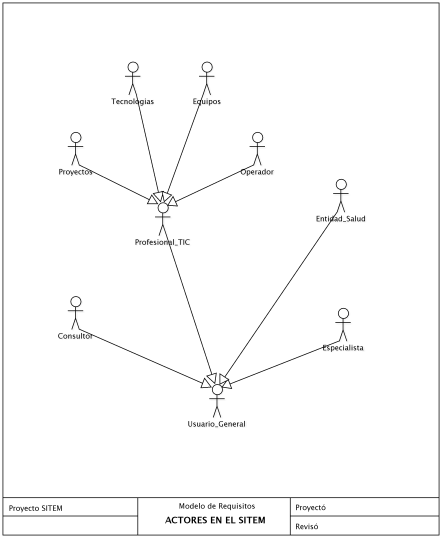
\includegraphics[width=156mm, height=182mm]{actores.png}
 \caption{Conjunto de Actores de OpenSITE;}
 \label{actores}
\end{figure}

\subsection{Casos de Usos}
Los artefactos correspondientes a los casos de uso se han empaquetado de acuerdo al tipo de nodo en el cual se desarrollan. Se incluyen solo los casos que se consideran nucleares y las especificaciones de mayor relevancia e impacto.

\begin{figure}
 \centering
 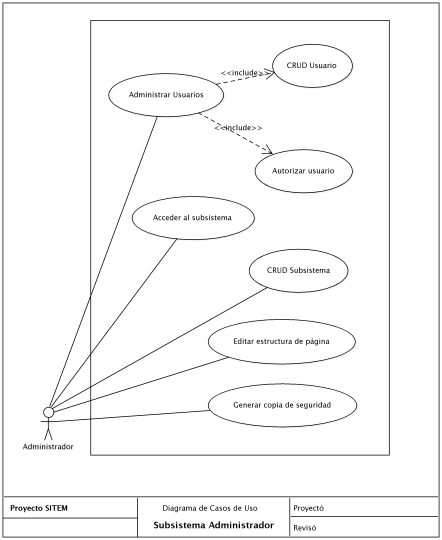
\includegraphics[width=156mm, height=182mm]{casos_admin.png}
 \caption{Casos de uso principales del Actor administrador}
 \label{casos_admin}
\end{figure}

\begin{figure}
 \centering
 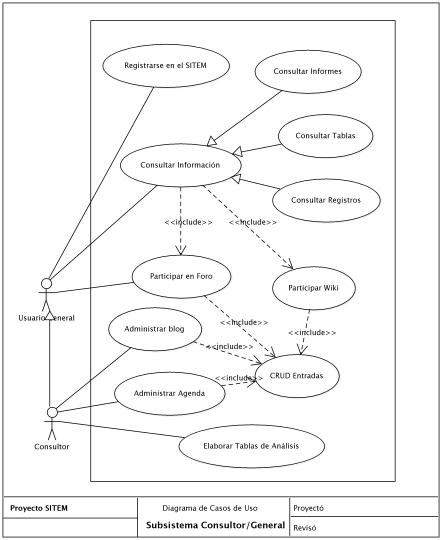
\includegraphics[width=156mm, height=182mm]{casos_consultor.png}
 \caption{Casos de uso principales del Actor Consultor/Usuario General}
 \label{casos_consultor}
\end{figure}

\begin{figure}
 \centering
 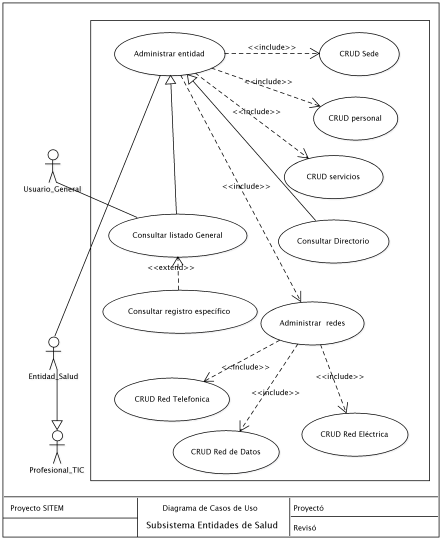
\includegraphics[width=156mm, height=182mm]{casos_entidad.png}
 \caption{Casos de uso principales del Actor Entidad de Salud}
 \label{casos_entidad}
\end{figure}

\begin{figure}
 \centering
 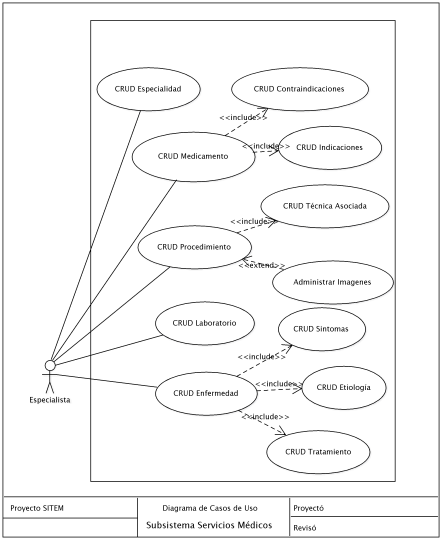
\includegraphics[width=156mm, height=182mm]{casos_servicios.png}
 \caption{Casos de uso principales del Actor Servicios Médicos}
 \label{casos_servicios}
\end{figure}

\begin{figure}
 \centering
 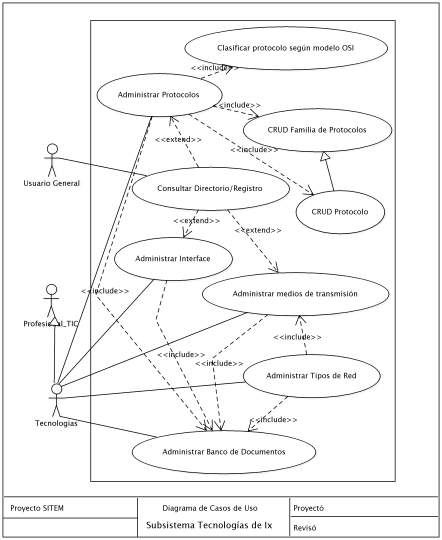
\includegraphics[width=156mm, height=182mm]{casos_tecnologias.png}
 \caption{Casos de uso principales del Actor Tecnologías de Interconexión}
 \label{casos_tecnologia}
\end{figure}

\begin{figure}
 \centering
 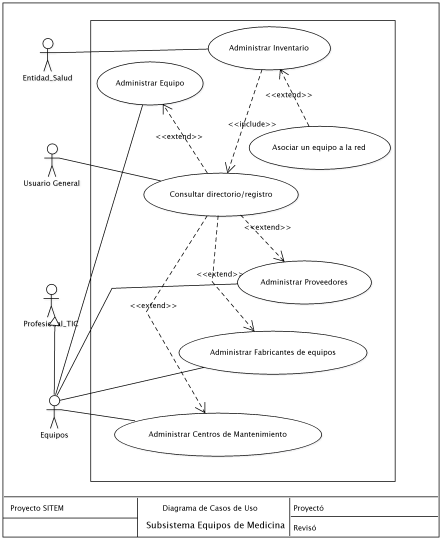
\includegraphics[width=156mm, height=182mm]{casos_equipos.png}
 \caption{Casos de uso principales en el Subsistema Equipos de Medicina}
 \label{casos_equipos}
\end{figure}

\begin{figure}
 \centering
 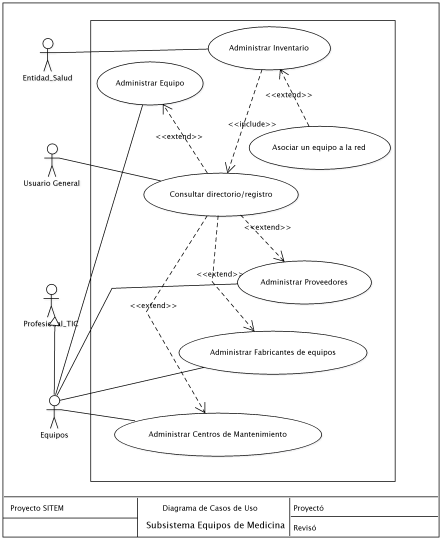
\includegraphics[width=156mm, height=182mm]{casos_equipos.png}
 \caption{Casos de uso principales en el Subsistema de Operadores de Servicios de Telecomunicaciones}
 \label{casos_telecomunicaciones}
\end{figure}

\chapter{Modelo de Análisis y Diseño}
\label{modelo_analisis}
\section{Especificaciones de Casos de Usos}

Para analizar en detalle los requerimientos del sistema se especifica mediante plantillas aquellos casos de uso que se consideran de importancia para el desarrollo base - conocidos como \textit{Casos de Uso Nucleares}. La tabla \ref{tabla_plantilla} muestra las secciones básicas que contiene un caso de uso. En aquellos casos de uso que una o varias secciones carezcan de contenido relevante se omiten por completo su declaración.

\begin{table}
\begin{center}
\begin{tabular}{|l|p{10cm}|}
\hline
\textbf{Caso de Uso}&\\
\hline
Nombre & Nombre que identifica el caso de Uso usualmente es el mismo utilizado en el diagrama de Casos de Uso\\
\hline
Objetivo & Beneficio que obtiene el actor con la ejecución de este caso de uso.\\
\hline
Código Interno & Código único que identifica al Caso de Uso dentro del repositorio de artefactos.\\
\hline
Actores & Usuarios que intervienen en el caso de uso\\
\hline
Precondiciones & Estado en que debe encontrarse el SITEM antes de ejecutarse el caso de uso.\\
\hline
Flujo Básico & Flujo principal de actividades. Ambiente ideal.\\
\hline
Flujo Alternativo y de error & Actividades que bifurcan el flujo básico. Si existe más de un flujo alternativo este debe colocarse en una nueva fila.\\
\hline
Postcondiciones & Estado en que queda el SITEM después de ejecutado el caso de uso.\\
\hline
Puntos de Extensión & Secuencias de acciones que extienden el flujo del caso de uso.\\
\hline
\end{tabular}
\caption{Plantilla Genérica para la Especificación de los Casos de Uso.}
\label{tabla_plantilla} 
\end{center}
\end{table}


\begin{table}
\begin{center}
\begin{tabular}{|l|p{10cm}|}
\hline
\textbf{Caso de Uso}&\\
\hline
Nombre & Registrarse en el SITEM\\
\hline
Objetivo & El actor logra crear una cuenta en el SITEM con un rol específico para poder trabajar en un subsistema dado.\\
\hline
Código Interno & UC-GENERAL-001 \\
\hline
Actores & Usuario General\\
\hline
Precondiciones & Ninguna.\\
\hline
Flujo Básico & 1. El usuario general selecciona la opción de nuevo usuario desde la página principal del SITEM.\\
& 2. El SITEM muestra un formulario con los campos:\\
& Nombres\\
& Apellidos\\
& Correo Electrónico\\
& Teléfono\\
& Nombre de Usuario\\
& Clave\\
& Reescriba la clave\\
& Acceso Requerido\\
& 3. El usuario diligencia uno a uno los campos requeridos y opcionales.\\
& 4. El usuario envía los datos al SITEM.\\
& 5. El SITEM verifica que los datos tengan los formatos esperados.\\
& 6. El SITEM ingresa el registro a la base de datos colocando el campo de estado en 1 - registrado sin autorización.\\
& 7. El SITEM redirecciona a la página de registro exitoso.\\
& 8. El usuario acepta el mensaje.\\
\hline
Postcondiciones & Se agregó un registro en la base de datos con el campo de estado en 1.\\
\hline
Casos de uso relacionados&Seleccionar Rol en el SITEM\\
\hline
\end{tabular}
\caption{Caso de Uso Registrarse en el SITEM}
\label{casouso1} 
\end{center}
\end{table}

\begin{table}
\begin{center}
\begin{tabular}{|l|p{10cm}|}
\hline
\textbf{Caso de Uso}&\\
\hline
Nombre & Administrar autorizaciones de Usuario\\
\hline
Objetivo & Proveer un mecanismo eficaz para que el administrador general del SITEM pueda gestionar el estado de autorización de los usuarios en los diferentes subsistemas.\\
\hline
Código Interno & UC-GENERAL-002 \\
\hline
Actores & Administrador\\
\hline
Precondiciones & Debe existir por lo menos un usuario registrado en el sistema diferente al administrador.\\
& El administrador se encuentra correctamente autenticado y autorizado en el subsistema de administrador.\\
\hline
Flujo Básico & 1. El Administrador selecciona la opción Usuarios desde el menú principal del subsistema Administrador.\\
& 2. El SITEM muestra un listado con los datos básicos de diferentes usuarios registrados:\\
& Nombres\\
& Apellidos\\
& Correo Electrónico\\
& Acceso Requerido\\
& 3. \textit{Punto de Extensión} 1.\\
& 4. \textit{Punto de Extensión} 2.\\
& 5. El administrador verifica que los datos del usuario son reales.\\
& 6. El administrador seleccionada la casilla de verificación y acepta el trámite.\\
& 7. El SITEM procesa el formulario colocando el estado del usuario en valor 2 - Registrado y Autorizado.\\
& 8. El SITEM indica con un mensaje el éxito en la operación de autorización.\\
& 9. El SITEM envía un mensaje de texto al usuario indicando que ha sido autorizado.\\
& 8. El Administrador acepta el mensaje de éxito.\\
\hline
Postcondiciones & Se cambia el valor en el campo estado del registro correspondiente al usuario.\\
\hline
Puntos de Extensión & 1:direccion=“avanzar” o direccion=“retroceder” extend Navegar en listado. \\
& 2:Opción=“buscar” extend Busqueda condicional de registro. \\
\hline
\end{tabular}
\caption{Caso de Uso Autorizar un usuario para acceder al SITEM}
\label{casouso2} 
\end{center}
\end{table}

\begin{table}
\begin{center}
\begin{tabular}{|l|p{10cm}|}
\hline
\textbf{Caso de Uso}&\\
\hline
Nombre & Generar Copia de Seguridad\\
\hline
Objetivo & Generar una copia de seguridad de los datos contenidos en la base de datos asociada al SITEM.\\
\hline
Código Interno & UC-GENERAL-003 \\
\hline
Actores & Administrador\\
\hline
Precondiciones & El administrador se encuentra correctamente autenticado y autorizado en el subsistema de administrador.\\
\hline
Flujo Básico & 1. El Administrador selecciona la opción Copia de Seguridad el menú principal del subsistema Administrador.\\
& 2. El SITEM muestra un listado con las tablas opcionales para la copia de seguridad.\\
& 3. El administrador selecciona la casilla de verificación de las tablas que desea sean copiadas.\\
& 4. \textit{Punto de Extensión} 1.\\
& 5. El administrador acepta la selección.\\
& 6. El SITEM muestra un listado con las tablas que serán copiadas y un formulario con los campos:\\
& Nombre del Archivo.\\
& Ruta de Descarga.\\
& 7. El usuario diligencia uno a uno los campos requeridos.\\
& 8. El usuario envía los datos al SITEM.\\
& 9. El SITEM realiza una copia de los registros escribiéndolos uno a uno en los archivos de destino.\\
& 10. El SITEM redirecciona a la pagina de operación exitosa.\\
& 11. El usuario acepta el mensaje.\\
\hline
Postcondiciones & Se crea n archivos en la carpeta de destino con el contenido de las n tablas seleccionadas para copia de seguridad.\\
\hline
Puntos de Extensión & 1:opcion=“todo” extend Seleccionar todos los cuadros.\\
\hline
\end{tabular}
\caption{Caso de Uso realizar Copia de Seguridad}
\label{casouso3} 
\end{center}
\end{table}

\begin{table}
\begin{center}
\begin{tabular}{|l|p{10cm}|}
\hline
\textbf{Caso de Uso}&\\
\hline
Nombre & Elaborar Tablas de Análisis\\
\hline
Objetivo & Obtener un repositorio de análisis de algún componente del modelo jerárquico de seguimiento a proyectos.\\
\hline
Código Interno & UC-GENERAL-004 \\
\hline
Actores & Consultor\\
\hline
Precondiciones & Existe en el SITEM un modelo jerárquico de seguimiento a proyectos.\\
\hline
Flujo Básico & 1. El Consultor selecciona la opción Seguimiento desde el menú principal del subsistema Consultor.\\
& 2. El SITEM muestra el modelo de seguimiento a proyectos con sus componentes de primer nivel.\\
& 3. \textit{Punto de Extensión} 1.\\
& 4. El Consultor selecciona la opción de Analizar para un componente.\\
& 5. El SITEM muestra un formulario con los campos:\\
& Valoración Cualitativa.\\
& Valoración Cuantitativa.\\
& Juicio.\\
& Diagnóstico.\\
& Fortalezas.\\
& Oportunidades.\\
& Debilidades.\\
& Amenazas.\\
& Directrices de Mejoramiento.\\
& Directrices de Acción.\\
& 6. El usuario diligencia uno a uno los campos requeridos y opcionales.\\
& 8. El usuario envía los datos al SITEM.\\
& 5. El SITEM verifica que los datos tengan los formatos esperados.\\
& 6. El SITEM ingresa el registro a la base de datos.\\
& 7. El SITEM redirecciona a la página de registro exitoso.\\
& 8. El usuario acepta el mensaje.\\
\hline
Postcondiciones & Existe un registro de análisis asociado a un componente y un consultor.\\
\hline
Puntos de Extensión & 1:opcion=“mas” extend Mostrar Componentes de Nivel Inferior\\
\hline
\end{tabular}
\caption{Caso de Uso Elaborar Tablas de Análisis}
\label{casouso4} 
\end{center}
\end{table}

\begin{table}
\begin{center}
\begin{tabular}{|l|p{10cm}|}
\hline
\textbf{Caso de Uso}&\\
\hline
Nombre & Ingresar una Entidad\\
\hline
Objetivo & Registrar una nueva entidad de Salud en el SITEM.\\
\hline
Código Interno & UC-GENERAL-005 \\
\hline
Actores & Entidad Salud\\
\hline
Precondiciones & El usuario Entidad Salud se encuentra autorizado y autenticado en el subsistema Entidades de Salud.\\
\hline
Flujo Básico & 1. Entidad Salud selecciona la opción Nueva Entidad desde el menú principal del subsistema Entidades de Salud.\\
& 2. El SITEM muestra un formulario con los campos:\\
& Nombre de la Entidad.\\
&Nombre Corto.\\
&Logosímbolo.\\
&NIT.\\
&Fecha de Fundación.\\
&Dirección Principal.\\
&Teléfono Principal (PBX).\\
&Misión.\\
&Visión.\\
&Descripción.\\
&Comentarios.\\
& 3. El usuario diligencia uno a uno los campos requeridos y opcionales.\\
& 4. El usuario envía los datos al SITEM.\\
& 5. El SITEM verifica que los datos tengan los formatos esperados.\\
& 6. El SITEM comprueba que no exista otra Entidad registrada con el mismo NIT.\\
& 7. El SITEM ingresa el registro a la base de datos.\\
& 8. El SITEM redirecciona a la página de registro exitoso.\\
& 9. El usuario acepta el mensaje.\\
\hline
Flujo Alternativo & 5.A. Los datos no tienen el formato adecuado. \\
& 6.A. El SITEM informa el error.\\
& 7.A. \textit{Punto de Extensión} 1.\\
\hline
Flujo Alternativo & 6.A. Existe una entidad registrada con el mismo NIT. \\
& 7.A. El SITEM informa el error.\\
& 8.A. \textit{Punto de Extensión} 1.\\
\hline
Postcondiciones & Existe un registro de una entidad de salud.\\
\hline
Puntos de Extensión & 1:opcion=“corregir” extend Mostrar Formulario Corrección.\\
\hline
\end{tabular}
\caption{Caso de Uso Ingresar una Nueva Entidad de Salud.}
\label{casouso5} 
\end{center}
\end{table}

\begin{table}
\begin{center}
\begin{tabular}{|l|p{10cm}|}
\hline
\textbf{Caso de Uso}&\\
\hline
Nombre & Consultar información básica de una entidad de Salud.\\
\hline
Objetivo & Obtener en pantalla los datos básicos de una entidad de salud.\\
\hline
Código Interno & UC-GENERAL-006 \\
\hline
Actores & Entidad Salud, usuario general\\
\hline
Precondiciones & El usuario se encuentra autorizado y autenticado en el subsistema Entidades de Salud.\\
\hline
Flujo Básico & 1. Entidad Salud selecciona la opción Entidades desde el menú principal del subsistema Entidades de Salud.\\
& 2. El SITEM muestra un listado de 25 entidades ordenadas alfabéticamente por nombre.\\
& 3. \textit{Punto de Extensión} 1.\\
& 4. El usuario selecciona una entidad de salud desde el listado.\\
& 5. El SITEM realiza una búsqueda con el id de la entidad.\\
& 6. El SITEM muestra en pantalla el menú secundario para solicitar edición y los datos de la entidad:\\
& Nombre de la Entidad.\\
&Nombre Corto.\\
&Logosímbolo.\\
&NIT.\\
&Fecha de Fundación.\\
&Dirección Principal.\\
&Teléfono Principal (PBX).\\
&Misión.\\
&Visión.\\
&Descripción.\\
& 7. El usuario acepta los datos.\\
\hline
Puntos de Extensión & 1:direccion=“avanzar” o direccion=“retroceder” extend Navegar en listado. \\
\hline
\end{tabular}
\caption{Caso de Uso Consultar información básica de una entidad de Salud.}
\label{casouso6} 
\end{center}
\end{table}

\begin{table}
\begin{center}
\begin{tabular}{|l|p{10cm}|}
\hline
\textbf{Caso de Uso}&\\
\hline
Nombre & Editar un registro en el SITEM.\\
\hline
Objetivo & Editar la información que se encuentra en un registro del SITEM. La actualización puede involucrar más de una entidad en la capa de persistencia\\
\hline
Código Interno & UC-GENERAL-007\\
\hline
Actores & Profesional TIC, entidad salud, administrador, usuario general\\
\hline
Precondiciones & El usuario se encuentra autorizado y autenticado en el subsistema.\\
\hline
Flujo Básico & 1. El usuario selecciona la opción Editar Registro desde el menú secundario del subsistema.\\
& 2. El SITEM muestra un formulario rellenado con los datos del registro correspondiente.\\
& 3. El usuario editada los valores dentro de los controles del formulario.\\
& 4. El usuario envia el formulaenvíal SITEM.\\
& 5. El SITEM verifica que los datos editados no violen alguna regla de integridad referencial.\\
& 6. El SITEM actualiza los registros en la capa de persistencia.\\
& 7. El SITEM muestra al usuairo un mensausuarioxito.\\
& 8. El usuario acepta el mensaje.\\
\hline
Flujo Alternativo & 5.A. Existe un error de integridad referencial. \\
& 7.A. El SITEM informa el error.\\
& 8.A. \textit{Punto de Extensión} 1.\\
\hline
Puntos de Extensión & 1:opcion=“corregir” extend Mostrar Formulario Corrección.\\
\hline
Postcondiciones & Se actualizan los registros correspondientes.\\
\hline
\end{tabular}
\caption{Caso de Uso Editar un registro en el SITEM}
\label{casouso7} 
\end{center}
\end{table}

\begin{table}
\begin{center}
\begin{tabular}{|l|p{10cm}|}
\hline
\textbf{Caso de Uso}&\\
\hline
Nombre & Asociar un protocolo de comunicaciones al modelo OSI.\\
\hline
Objetivo & Asociar un protocolo de comunicaciones al modelo de referencia OSI.\\
\hline
Código Interno & UC-GENERAL-008\\
\hline
Actores & Profesional TIC, Tecnologías.\\
\hline
Precondiciones & El usuario se encuentra autorizado y autenticado en el subsistema.\\
& Existe registrado por lo menos un protocolo de comunicaciones en el SITEM.\\
\hline
Flujo Básico & 1. El usuario selecciona la opción \textbf{Más Información} desde el menú secundario del subsistema.\\
& 2. El SITEM muestra la información del protocolo asociada por áreas temáticas.\\
& 3. El usuario selecciona la opción Clasificar OSI.\\
& 4. El SITEM muestra el grafico de siete capgráficomodelo OSI.\\
& 5. El usuario selecciona una o varias capas del modelo.\\
& 6. El SITEM asocia el id del protocolo a cada una de las capas del modelo OSI seleccionadas por el usuario.\\
& 7. El SITEM muestra el modelo OSI extendido con los demás protocolos registrados en cada capa.\\
& 8. El usuario acepta el registro.\\
\hline
Flujo Alternativo & 5.A. El usuario no selecciona ninguna capa. \\
& 7.A. El SITEM regresa al punto 2 del caso de uso.\\
\hline
Postcondiciones & El conjunto de protocolos asociados a una capa del modelo OSI se incrementa.\\
\hline
\end{tabular}
\caption{Caso de Uso Asociar un protocolo de comunicaciones al modelo OSI.}
\label{casouso8} 
\end{center}
\end{table}

\begin{table}
\begin{center}
\begin{tabular}{|l|p{10cm}|}
\hline
\textbf{Caso de Uso}&\\
\hline
Nombre & Borrar un registro del SITEM.\\
\hline
Objetivo & Eliminar un registro en algún subsistema del SITEM garantizando que solo el experto en información lo realice y se mantenga la integridad referencial en los datos.\\
\hline
Código Interno & UC-GENERAL-009\\
\hline
Actores & Profesional TIC, Entidad Salud, Consultor, Administrador.\\
\hline
Precondiciones & El usuario se encuentra autorizado y autenticado en el subsistema.\\
& Existe un registro en el SITEM.\\
& El usuario a creado el registro y este no tiene información asociada.\\
\hline
Flujo Básico & 1. El usuario selecciona la opción \textbf{Eliminar Registro} desde el menú secundario del subsistema.\\
& 2. El SITEM muestra un mensaje de conformación de eliminación con los datos básicos del registro.\\
& 3. El usuario selecciona la opción de \textbf{Confirmar Borrado}.\\
& 4. El SITEM elimina el registro cumpliento las restrcumpliendoe claves foraneas.\\
& 5. El foráneasestra un mensaje indicando que el registro se ha borrado del sistema.\\
& 6. El usuario acepta el mensaje.\\
& 7. El SITEM redirecciona a la página en donde se encontraba el usuario antes del proceso de borrado.\\
\hline
Flujo Alternativo & 3.A. El usuario no acepta borrar el registro. \\
& 4.A. Continua en el punto 7 del flujo principal.\\
\hline
Postcondiciones & El registro se borra del sistema.\\
\hline
\end{tabular}
\caption{Caso de Uso para Borrar un registro en el SITEM.}
\label{casouso9} 
\end{center}
\end{table}

\begin{table}
\begin{center}
\begin{tabular}{|l|p{10cm}|}
\hline
\textbf{Caso de Uso}&\\
\hline
Nombre & Acceder a una página del SITEM.\\
\hline
Objetivo & Ingresar a una página específica dentro del sistema.\\
\hline
Código Interno & UC-GENERAL-010\\
\hline
Actores & Profesional TIC, Entidad Salud, Consultor, Administrador.\\
\hline
Precondiciones & El usuario está autorizado para acceder a la página.\\
& La página se encuentra registrada en el SITEM.\\
& La página tiene uno o más bloques asociados.\\
\hline
Flujo Básico & 1. El usuario elige un enlace a una página dentro del SITEM.\\
& 2. El SITEM verifica que el usuario tiene una sesión  válida\\
& 3. El SITEM rescata los valores de la página desde la base de datos.\\
& 4. El SITEM verifica que el usuario tenga los privilegios necesarios para ingresar a la página.\\
& 5. El SITEM consulta la estructura de la página desde la base de datos.\\
& 6. El SITEM envía secuencialmente el código HTML correspondiente a cada una de los bloques que constituyen la página.\\
& 7. El SITEM registra el acceso del usuario en la base de datos.\\
& 8. El SITEM actualiza la información de sesión.\\
\hline
Flujo Alternativo & 4.A. El usuario no tiene los privilegios para ver la página. \\
& 5.A. El SITEM registra un atento de ingreso ilegal.\\
& 6.A. El SITEM muestra un mensaje informando el error.\\
\hline
Postcondiciones & El usuario ingresa a una página dentro del SITEM.\\
\hline
\end{tabular}
\caption{Caso de Uso para Acceder a una página del SITEM.}
\label{casouso10} 
\end{center}
\end{table}
\chapter{Modelo de Implementación}
\label{modelo_implementacion}

El modelo de implementación del SITEM esta compuesto básicamente por los siguientes artefactos que en su conjunto representan lo que comunmente se denomina el aplicativo:
\begin{itemize}
\item \textbf{Bloques:} Unidad Básica de funcionalidad. Se pueden pensar en ellos como “instancias” persistentes de clases abstractas. En especial se tienen tres clases:
\begin{itemize}
\item Administración: Con atributos y métodos para mostrar directorios de datos.
\item Menú: Con métodos especializados en la administración de enlaces dentro del SITEM.
\item Registro: Para la realización de casos CRUD.
\end{itemize}
\item \textbf{Clases}: Descriptores para varios tipos de objetos entre las cuales se tiene:
\begin{itemize}
\item DBMS: Interaccción con la bases de datos.
\item Página: Describe objetos que realizan la construcción en tiempo de ejecución de las páginas.
\item Encriptar: Descriptor para objetos que se encargan de codificar y decodificar los datos en el SITEM. El conjunto de operaciones debe ser manipulado en cada implementación del SITEM para garantizar un alto nivel de seguridad.
\item Autenticacion: Con descripción de atributos y operaciones que controlan las rutinas de AAA en el SITEM.
\item Config: Clasificador de objetos que manipulan las variables de configuración globales.
\item Html: Descriptor de controles de formularios en el SITEM.
\item Sesión: Operaciones y atributos para el control de sesiones en el SITEM luego del proceso de AAA.
\item Mensaje: Para objetos que administran mensajes de interacción con los actores.
\item Sql: Clase para describir objetos especializados en gestionar archivos con extensión SQL.
\item Navegacion: Con operaciones específicas para el control de desplazamiento entre conjuntos de registros.
\end{itemize}
\item \textbf{Función:} Métodos JavaScript para la validación y control de navegación en el lado del cliente.
\item \textbf{Estilo:} Para el control de la capa de Interfaz Gráfica.
\end{itemize}

\begin{figure}
 \centering
 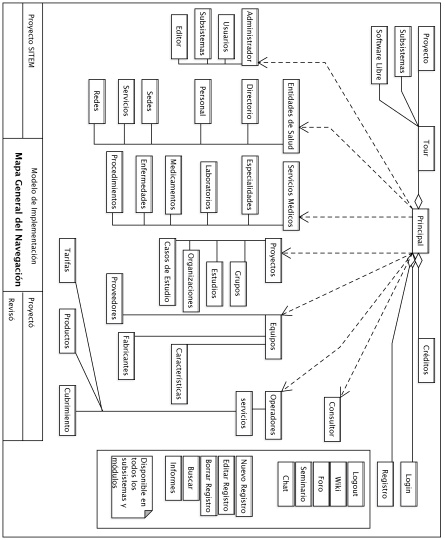
\includegraphics[width=156mm, height=182mm]{mapa_navegacion.png}
 \caption{Modelo General de Navegación}
 \label{mapa_navegacion}
\end{figure}

\section{Código Fuente del SITEM}

La siguiente porción de código fuente representa el formato general que se encuentra en el SITEM. Por patrón general se recomienda a todos los grupos que participan en el desarrollo que mantengan un esquema de codificación claro y documentación \textit{in situ} suficiente para aclarar secciones.

\subsection{Clase Página}

La clase Página tiene las operaciones:
\begin{itemize}
\item pagina: Constructor.
\item especificar pagina: Inicializar variables privadas.
\item procesar pagina: Controlar redireccionamientos.
\item ancho seccion: Implementa control de secciones colapsadas.
\item armar seccion: Para seleccionar los bloques que contiene cada página.
\end{itemize}

Algunos métodos instancian la clase DBMS y HTML. Estas por lo tanto deben ser visibles.
\begin{verbatim*}

class pagina
{

	//Metodo constructor
	function pagina(id_pagina,configuracion)
	{
		//Declaracion de variable parta controlar accesos indebidos
		GLOBALS["autorizado"]=TRUE;
		this->especificar_pagina(id_pagina);
		
		if(!isset(_POST['registro_compuesta']))
		{
			if(!isset(_REQUEST['action']))
			{
				
				this->mostrar_pagina(configuracion);
			}
			else
			{
				//echo 'Procesamiento de la pagina';
				this->procesar_pagina(configuracion);
			}
		}
		else
		{
			this->mostrar_pagina(configuracion);		
		}
	}
	//Fin del metodo constructor
	
	
	
	//Metodo especificar_pagina
	function especificar_pagina(id_pagina)
	{
	
		this->id_pagina=id_pagina;
	
	}
	//Fin del metodo especificar_pagina
.
.
.
} \end{verbatim*}
\chapter{Modelo de Datos}
\label{modelo_datos}

La capa de persistencia en el SITEM esta soportada en una estructura de base de datos de modelo Relacional. La forma normal básica - 3NF, se garantiza mientras que otras formas normales pueden ser omitidas en casos puntuales donde se demuestre, por pruebas de desempeño, que no seguirlas redunda en una mejora significativa de la velocidad en el acceso a los datos sin detrimento de la calidad e integridad de los mismos. A continuación se listan las formas normales tenidas en cuenta como patrón de diseño en el modelo de datos del SITEM:

\begin{itemize}
\item Primera Forma Normal: Cada renglón-columna contiene valores atómicos.
\item Segunda Forma Normal: 1NF y todo campo que no sea clave primaria depende de los campos clave.
\item Tercera Forma Normal: 2NF y no hay dependencias transitivas.
\item Forma Normal de Boyce-Codd: Todos los determinantes de la tabla son clave candidata.
\item Cuarta Forma Normal:  Una fila no debe contener dos o más campos multi-valorados.
\item Quinta Forma Normal: Una tabla puede almacenar atributos dependientes a la clave sólo por unión.
\end{itemize}

\begin{figure}
 \centering
 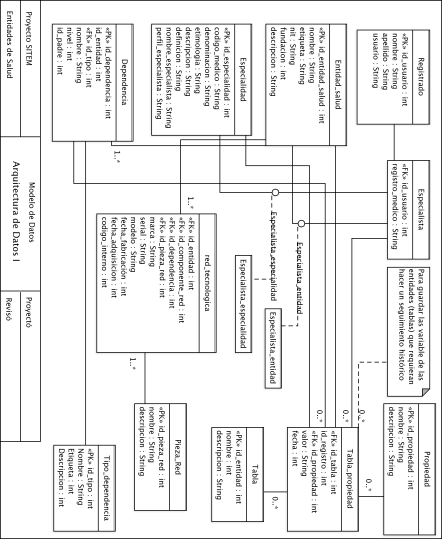
\includegraphics[width=156mm, height=182mm]{datos_entidad.png}
 \caption{Arquitectura de datos Subsistema Entidades de Salud}
 \label{mapanavegacion}
\end{figure}
\chapter{Modelo de Despliegue}
\label{modelo_despliegue}

\begin{figure}
 \centering
 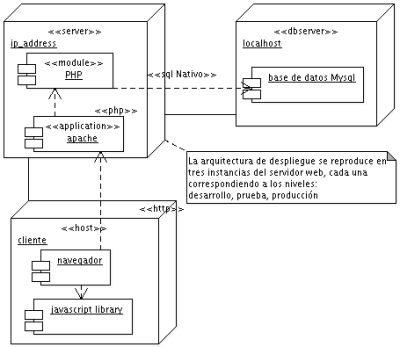
\includegraphics[width=141mm, height=122mm]{despliegue.png}
 \caption{Modelo de Despliegue}
 \label{despliegue}
\end{figure}

El SITEM se despliega sobre un servidor que tenga instalado un programa que acepte peticiones usando el protocolo HTTP - Servidor Web, tenga soporte para el interprete de PHP y un servidor de bases de datos MySQL o PostgreSQL. La figura \ref{despliegue} muestra el diagrama de componentes correspondiente a la arquitectura propuesta.

La arquitectura mostrada se reproduce en tres instancias del servidor web, cada una correspondiendo a los niveles de:

\begin{itemize}
\item \textbf{Desarrollo:} Con las versiones más recientes del sistema que se consideran en versión alfa o inestables. Dentro de la codificación son aquellas que muestran incrementos en el cuarto segmento: AA.XX.YY.\textbf{ZZ}
\item \textbf{Prueba:} Versiones que tienen desarrollos estables pero que aún no han pasado la etapa de revisión de casos de prueba. En la codificación son aquellas que muestran un incremento en el tercer segmento: AA.XX.\textbf{YY}.ZZ 
\item \textbf{Producción:} Versiones que han sido probadas y no tienen errores detectados. De acuerdo a la naturaleza de la funcionalidad alcanzada estas versiones representan un incremento en los segmentos primero o segundo dentro de la codificación. 

Si es el primer segmento el que incrementa se alcanza un ciclo de desarrollo y la versión es bautizada con un nombre específico. Para el SITEM se usan los nombre de los Dioses maya que participaron en alguno de los tres intentos por crear la humanidad.
\end{itemize}

\chapter{Instrumento Preliminar para la Fase de Transición}
\label{formulario_preliminar}

\section{Presentación}

El presente instrumento agrupa de una manera lógica los aspectos necesarios para identificar el estado y potencialidad de los servicios de salud que hacen uso intensivo de las TIC. El contenido está basado en aquel utilizado por el proyecto HERMES, modelo completamente depurado que ha servido de base para la recolección de información de varios proyectos de telemedicina emprendidos en la Comunidad Económica Europea (CEE). Así mismo se le han adicionado algunos ítem aplicables al contexto colombiano.

\subsection{Indicaciones Generales}

El cuestionario deberá ser respondido como fase posterior a la etapa de divulgación del proyecto y una vez se haya conformado un comité, o en su defecto, se haya designado un encargado, por parte de la institución objetivo. Es necesario que en el proceso los miembros del proyecto sirvan de apoyo resolviendo de una manera exacta las dudas que surjan en el ámbito tecnológico (telesalud, estándares de telecomunicaciones y otros). De igual forma se deben realimentar de la información especializada que puedan capturar de los comités. Para apoyar estas tareas podrán hacer uso de las herramientas de trabajo en grupo que se encuentran en el Portal SITEM.

La profundidad con que se respondan las cuestiones garantiza que la institución evalúe su situación actual frente a la posible implementación de servicios de salud prestados en la modalidad de Telemédicina.

El cuestionario esta disponible para ser diligenciado en línea de tal forma que podrá ser resuelto en cualquier orden y anexando cualquier tipo de información que se considere conveniente para aclarar y/o complementar una respuesta. 

Las cuestiones deberán ser manejadas por un especialista en la materia aunque esto conduzca a que los encargados del proyecto jueguen un papel meramente coordinador de actividades. Todas las cuestiones deben ser tenidas en cuenta aunque se hayan tratado tácitamente en respuestas anteriores.

\subsection{Contexto Clínico}

Las preguntas que tienen que ver con los servicios clínicos están incluidos en este cuestionario dado que uno de sus objetivos es dar un conocimiento global del sistema de telemedicina y sus características. 

El cuestionario puede ser usado para ver el estado actual de los aspectos clínicos y para evaluar cuales mejoras deben ser hechas. Las preguntas no pretenden definir competencias clínicas y son por lo tanto abiertas y basadas en la familia de estándares de calidad ISO 9000. Estas características están en consonancia con el concepto de Administración con Calidad Total  (TQM):

\begin{enumerate}
\item Definición de necesidades
\item Planificación para cubrir necesidades.
\item Controles para cubrir los estándares.
\item Mejora continua
\end{enumerate}

Un gran número de factores deben ser tomados en mente en consideración a los tópicos relacionados en esta sección:

Los estándares médicos deben definir el contexto sobre el cual el sistema de telemedicina ha de ser introducido, no solamente las necesidades que han de ser atendidas por dicho servicio. Es decir, la definición de estándares médicos y de un conjunto de directrices para asegurar la más alta calidad en la atención debe ser una actividad independiente del sistema de telemedicina a implementar.

Cualquier servicio medico en la modalidad de telemedicina que se quiera implementar en un ambiente donde existe un conjunto aceptado y aplicado de estándares médicos y directrices, debe estar completamente estructurado para que sea compatible. Si no lo es debe estar lo suficientemente documentado y la necesidad de su aplicación claramente dilucidada.

Es necesario tener en cuenta las siguientes definiciones:

\begin{description}
\item[Evento de Atención en Salud]
Un contacto para el cuidado de la salud que requiere que un servicio clínico sea aplicado.

\item [Servicio Clínico]
Uno a más planes de salud autorizados e implementados para poder llenar los requerimientos del evento de atención en salud.

\item [Plan de salud]
Uno o más procedimientos clínicos asociados a estándares médicos y directrices que se utilizan para poder cubrir un servicio médico.

\item [Procedimiento clínico]
Una o más actividades de tratamiento en salud.

\item [Directriz médica]
Un informe sistemáticamente desarrollado, el cual asiste en la toma de decisiones acerca de los procedimientos a seguir para una condición clínica específica. 

\item [Estándar médico] 
Un documento, establecido por consenso y aprobado por un cuerpo consultor organizado, el cual provee para el uso común y repetido de las pautas o las características de actividades de cuidados clínicos (o sus resultados)  y su objetivo principal es el de alcanzar el grado óptimo de orden en un contexto de medicina dado.
\end{description}

\subsubsection{Unidades de Recolección de Información}


\begin{enumerate}
\item ¿Cuales son los servicios de salud por modalidad telemédicina que deben ser implementados?

Describa sus ideas/necesidades para el uso de la telemedicina en su ambiente de trabajo 
\begin{itemize}
\item ¿Cuales son los servicios clínicos que serán afectados o reemplazados por el nuevo sistema de telemedicina?
\item ¿Cuales organizaciones/departamentos clínicos están directamente involucrados en el servicio? 
\end{itemize}

\item ¿Cuales son los requerimientos de los usuarios?
\begin{itemize}
\item  ¿Quienes son los usuarios? 

Quien está involucrado.

\item ¿Qué hacen ellos?
roles/actividades 
Usuarios Cliente (pacientes) 
Usuarios participantes (doctores, enfermeros, paramédicos,  personal de soporte, etc.) 

\item  ¿Que método era usado para obtener los requerimientos clínicos de los usuarios? 

Ejemplo: ¿ Existe un grupo de usuarios, incluyendo un representante del paciente, donde se use un cuestionario o se realice una encuesta?

\item ¿Cuales son los eventos/episodios clínicos que serán dirigidos en el sistema de telemedicina? 

\item ¿Que señales, incluyendo signos vitales, necesitarán ser monitorizados? 

\item ¿Qué equipo es necesario para monitorizar dichas variables? 

\item ¿Qué procedimientos (incluyendo entrenamiento) son requeridos para implementar la monitoria de las variables? 

\item ¿Quién interpretará la información monitorizada? (Especificar el nivel profesional) 

\item ¿Que factores son requeridos para garantizar la seguridad del paciente, exactitud y funcionalidad de los equipos, y aceptación por parte del usuario en la monitoria y otros procedimientos?

\end{itemize}

\item  ¿Cuales son los procedimientos de servicios clínicos que podrán ser afectados por la implementación de la telemedicina?
 
Ejemplo: El acceso al servicio,  referencia, admisión, descarga y procedimientos de seguimiento. 

Describir los eventos y procedimientos existentes, además de las particularidades del ambiente local (específicas) 

Describir una aproximación al nuevo sistema de telemedicina (tomando en consideración condiciones y directrices locales) 

Describir la estrategia  con la cual se obtendrá la aprobación local y extendida de los cambios. 

\item ¿Cuales son los estándares/ pautas relacionadas con el sistema de telemedicina?

Pautas existentes que deben ser conservadas en el sistema de telemedicina. 

Pautas que deben ser reemplazadas. 

\begin{itemize}
\item ¿Existen nuevas directrices que deban ser creadas para implementar el sistema de telemedicina? 

\item ¿Que proceso de desarrollo de directrices debería ser usado?

\end{itemize}

\item ¿Cuales son los recursos humanos requeridos por el sistema de telemedicina? 

\begin{itemize}
\item ¿El sistema de telemedicina puede ser implementado y operado por el personal existente? 

\item ¿Nuevo personal debe ser entrenado?
\end{itemize}

\item ¿Cuales son las necesidades de entrenamiento para el sistema de telemedicina?

En telemática, telemedicina, procedimientos de calidad, análisis de requerimientos, indicadores de resultados y desempeño, etc. 

Tipo de entrenamiento requerido.

Tipo y grado del personal.
\end{enumerate}

\subsection{ Contexto de servicio / relación con el entorno}

Es necesario definir una estrategia de desarrollo para poder garantizar que la solución en Telemedicina encaje perfectamente en el ambiente existente de servicios en salud. Los servicios Telemédicos usualmente se montan sobre alguno de los siguientes escenarios: Creación de nuevos servicios Telemédicos ó servicio telemédico que reemplazará un servicio no telemédico existente.

\subsubsection{Unidades de Recolección de Información}

\begin{itemize}
\item Restricciones legales. 

La pregunta explora las restricciones legales, éticas y sociales sobre el servicio y aquellos que participan en él. Las restricciones éticas pueden estar enmarcadas en leyes pero no siempre sucede, ej. Los médicos tienen límites éticos promulgados por organismos internacionales pero razones culturales pueden flexibilizar o endurecer dichas directrices,


\begin{enumerate}
\item ¿Cuales son las restricciones legales de los servicios telemédicos?

\begin{itemize}
\item Con respecto a las trasmisiones de datos. 
\item Con respecto a la protección de datos.
\item Con respecto a la responsabilidad en los productos y el seguimiento de estándares.
\item Con respecto a la libertad de información / privacidad 
\item Con respecto a la responsabilidad personal y organizativa. 
\item Con respecto a las entidades en las cuales se siguen responsabilidades legales. 
\item ¿Que organismos son responsables de la dirección legal? 
\end{itemize}

\item ¿Cuales son las consideraciones éticas

\begin{itemize}
\item ¿Para quien están dirigidas las restricciones éticas? 
\item ¿Con respecto a qué se definen dichas restricciones? 
\item ¿Que organismos son los encargados de la dirección en cuanto a cuestiones éticas?
\end{itemize}


\item ¿Cuales son los factores culturales y sociales a ser considerados?

\begin{itemize}
\item Consideraciones relacionadas con las raza. 
\item Consideraciones relacionadas con creencias culturales. 
\item Consideraciones relacionadas con el nivel educativo de los usuarios. 
\item Consideraciones relacionadas con el grupo socio económico al cual pertenece el usuario. 
\item Consideraciones relacionados con la ubicación geográfica de los usuarios. 
\item Consideraciones relacionadas con la edad de los usuarios.
\end{itemize}
\end{enumerate}

\item Consecuencias organizativas del sistema de telemedicina

La siguiente pregunta tiene que ver con los efectos que tendrá la introducción de un servicio de salud por modalidad de Telemedicina en la organización. 


\begin{enumerate}
\item ¿Que consecuencias tendrá en su organización la introducción del sistema de telemedicina? 

\begin{itemize}
\item Sobre la practica actual del trabajo.
\item Sobre los estándares locales. 
\item Sobre las inversiones existentes.
\end{itemize}

\item ¿Que características técnicas u organizativas requieren adaptación? 

\begin{itemize}
\item Practica actual del trabajo.
\item Estándares locales.
\item Inversiones existentes.
\item Políticas administrativas.
\item Maquinaria consultiva.
\end{itemize}

\end{enumerate}

\item ¿Que organizaciones/ contratistas deben interactuar para proveer el servicio de salud por modalidad de Telemedicina? 

\begin{itemize}
\item Organizaciones gubernamentales 
\item Administración regional de salud. 
\item Organizaciones públicas. 
\item Organizaciones profesionales. 
\item Organizaciones voluntarias (cruz roja, defensa civil, etc) 
\item Compañías de telecomunicaciones (Proveedores de servicios de interconexión) 
\item Compañías de seguros.
\item Otras compañías.
\end{itemize}
\end{itemize}

\subsection{Consideraciones Tecnológicas}

Esta sección esta relacionada con la definición de los recursos técnicos y de infraestructura necesarios para la provisión del sistema de telemedicina.

\subsubsection{Unidades de Recolección de Información}

\begin{enumerate}
\item Requerimientos de hardware

\begin{itemize}
\item ¿ Cuales plataformas de hardware son requeridas? (tanto como para proveer el servicio de salud en la modalidad de Telemedicina como para la utilización del mismo)

Ej.  PC, UNIX,  
\item  ¿Que tipo de almacenamiento se requiere? 
\begin{itemize}
\item  De acuerdo a la cantidad de información.
\item  De acuerdo a las políticas de seguridad.
\item  De acuerdo a la velocidad de búsqueda de la información.
\end{itemize}

\item  ¿Que tecnología de visualización se requiere?

\item  ¿Cuales son los requerimientos de procesamiento y como puede ser medido?
 

Ejemplo: Velocidad, procesamiento en paralelo. Medición en MFlops, Mips, Whetstones, Dhrystones o otras medidas estándar. 

\item ¿Que requerimientos especiales deben tener los equipos del usuario final?

Ej. Unidades móviles u otros dispositivos de usuario específicos (para captura de información, análisis, etc)

\item ¿Que puertos de comunicaciones deberán estar disponibles? 

Ejemplo: Ethernet, V32, SCSI, RS 232, USB, conectores especiales a otros equipos.

\item ¿Que tecnologías de adquisición, entrada o salida de datos son requeridas? 

Ej. Dispositivos de monitoria, modems, impresores, OCR, etc.

\item ¿Existen en su institución dispositivos que cumplan los requerimientos?

\end{itemize}


\item  Software 

\begin{itemize}
\item ¿Cuales sistemas operativos se requiere? 
\item ¿ Que herramientas de desarrollo son requeridas para desarrollar aplicaciones específicas para el sistema de telemedicina? 

Ejemplo: Lenguajes de programación, compiladores, enlazadores, depuradores, editores, herramientas CASE.
\end{itemize}

\item  ¿ Que infraestructura de comunicaciones se requiere? 
Ejemplo: Hardware de red, Software de red, 

\item  ¿ Que enlaces de comunicaciones se requiere? 
Ejemplo: Hardware (modems, bridges, switch, router,etc) 

\begin{itemize}
\item ¿ Que formatos? 
\item ¿ Que velocidad en los tiempos de respuesta? 
\item ¿ Que estándares / protocolos?
\item ¿ Que ancho de banda?
\end{itemize}

\item  Software aplicativo. 

\begin{itemize}
\item ¿ Cuales son los requerimientos para KBS, DSS? 
\item ¿ Cuales son los requerimientos para los sistemas de bases de datos? 
\item ¿ Cuales son los requerimientos para otro tipo de software aplicativo?
Ejemplo: ¿Existe software comercial, GNU, GPL que cubra las necesidades? 
\end{itemize}

\item  Requerimientos en infraestructura. 

\begin{itemize}
\item ¿ Que mobiliario se requiere? 
\item ¿ Que requerimientos eléctricos deben ser cumplidos?

Voltaje, corrientes, regulación, aislamiento, sistemas de tierra, etc.

\item ¿ Que temperatura, iluminación o humedad se requiere? 
\item ¿ Que cambios deben realizarse a los sitios existentes?
Ejemplo: Cableado, requerimientos de espacio, etc.
\end{itemize}

\item  ¿ Cuales metodologías están implementadas (o deben ser adoptadas) para cumplir los requerimientos tecnológicos y de infraestructura del servicio?                                                                                          \end{enumerate}


\subsection{Consideraciones de Calidad}

Esta sección contiene preguntas que deben ser contestadas para garantizar un servicio que tome en cuenta los factores de calidad en todas las etapas del proyecto.

\subsubsection{Unidades de Recolección de Información}

\begin{enumerate}
\item Aseguramiento de la calidad.
\begin{itemize}
\item ¿Cuales son las consideraciones de calidad a tener en cuenta en el sistema tele médico?

Ejemplo:. Mejoramiento de los mecanismos de cuidados para el paciente, mejoramiento de la eficiencia, reducción de costos, etc.

\item ¿Cuales métodos de administración con calidad total (TQM) existen o deben ser implementados? 

\item ¿Quien es responsable de la supervisión de los servicios médicos / de enfermería,  servicios técnicos, servicios administrativos y cuales son sus roles en el servicio telemédico?

\item ¿Como podría ser validado el sistema de telemedicina? 

Definir factores, variables, criterios e indicadores.

\item ¿Existen manuales y políticas de calidad implementadas para el sistema de telemedicina?

\item ¿Como podría obtenerse aprobación de la autoridades? 

Ejemplo: Legislación Local, Nacional o certificación ISO 
\end{itemize}


\item Grupo de usuarios

\begin{itemize}
\item ¿Está o estará un grupo de usuarios establecido para el sistema de telemedicina? 
\item ¿Esta o estará disponible un manual de usuario para el sistema de telemedicina? 
\item ¿Existirá enlaces entre los diversos grupos de usuarios nacionales/mundiales de servicios de salud similares brindados por la modalidad de telemedicina?
\end{itemize}


\item Describa las estrategias que se seguirán para dar conocimiento al público del nuevo servicio telemédico

\begin{itemize}
\item Estrategias para promocionar los objetivos del servicio y la forma de acceder a él.
\item Estrategias para el material educativo que será usado en el servicio. 
\item Estrategia para la mejora, promoción de resultados e impacto del servicio.
\end{itemize}

\item ¿Como podrían evaluarse las variables de calidad?
\item ¿Cuales son los valores aceptables para las variables de calidad seleccionadas ?
\item ¿Quien es el responsable de definir las estrategias de calidad?
\item ¿ Que tipo de documentación y procedimientos son usados (o se necesitan) para asegurar que la calidad total esta implementada?
\item ¿Que criterios pueden ser utilizados para demostrar que la calidad en el servicio es máxima? 
\end{enumerate}


\subsection{Aceptación del servicio de salud brindado en la modalidad de telemedicina}

\subsubsection{Unidades de Recolección de Información}

\begin{enumerate}
\item ¿ Qué tipos de intereses (beneficios) son inherentes al establecimiento de un sistema de telemedicina y que variables deben ser consideradas? 

Tipos de interés cuyos valores deben ser considerados: 

\begin{itemize}
\item Clínicos : Doctores, enfermeras, etc.
\item Tecnológicos: Técnicos, investigadores, doctores, desarrolladores, etc.
\item Éticos.
\item Económicos.
\item Industriales: Empresas, institutos de investigación/universidades, sociedad en general.
\end{itemize}

\item  ¿Qué hace que el sistema de telemedicina sea aceptado por las personas envueltas en el proyecto?

\item ¿Cual es el costo proyectado para establecer el sistema de telemedicina?

\begin{itemize}
\item Costos Capitales Tangibles: Equipos, instalación/pruebas, Cambios estructurales (Edificios/cuartos), cambios en la organización (Procedimientos), depreciación. 
\item Costos operativos: Personal, Servicio de Comunicaciones, mantenimiento y servicio, control de calidad, capacitación de personal, jornadas de socialización.
\end{itemize}

\item ¿Quien debería pagar por el establecimiento / implementación del sistema de telemedicina? 

Entre otros puede estar:

\begin{itemize}
\item Hospital, centros atención de salud.
\item Universidad.
\item Empresas de Telecomunicaciones.
\item Fundaciones de investigación. 
\item Proveedores de servicios de salud bajo la modalidad de telemedicina, compañías de aseguramiento.
\end{itemize}


\item ¿Cómo debe ser evaluado el sistema de telemedicina?

\begin{itemize}
\item Evaluación económica.
\item Evaluación de impacto social.
\item Evaluación de impacto médico.
\item Evaluación clínica.
\item Evaluación a las comunidades de práctica.
\end{itemize}

\item ¿Que técnicas de evaluación están disponibles?

\begin{itemize}
\item Investigación Evaluativa.
\item Evaluación Integral.
\item Etnografía.
\item Análisis de costos.
\item Análisis costo/beneficio.
\item Ingeniería económica.
\end{itemize}

\end{enumerate}


\subsection{Aspectos de Construcción y Persistencia del sistema de telemedicina}

\subsubsection{Unidades de Recolección de Información}

\begin{enumerate}
\item Tiempo de vida del proyecto

\begin{itemize}
\item ¿ Cual es el tiempo de vida proyectado para el sistema de telemedicina?
\item ¿ Que etapas pueden identificadas en dicho tiempo de vida?
\item ¿Cuánto tiempo tardaría en implementarse el servicio en una nueva ubicación?
\item ¿ Cuando y cuales mejoras pueden ser anticipadas / planeadas?
\end{itemize}
\item  ¿ Que recursos son o deben estar disponibles para establecer el sistema de telemedicina? 

\begin{itemize}
\item Recursos de información ( manuales, educación, soporte)
\item Recursos financieros.
\item Personal (Habilidades, incentivos, educación, entrenamiento) 
\item Espaciales (arquitectónicos)
\end{itemize}

\item  ¿ Que recursos deben ser re – evaluados?

\begin{itemize}
\item Financieros.
\item De personal.
\item Espaciales.
\item De cultura en la organización.
\item De mecanismos de interacción con el entorno.
\end{itemize}


\item Disponibilidad de los recursos para la operación del sistema de telemedicina. 

\begin{itemize}
\item ¿En que sitios? 
\item ¿En que tiempo?.
\item ¿Quien los suple?
\item ¿A quien o que van dirigidos?
\end{itemize}

\end{enumerate}


\subsection{Políticas de la Organización}

Esta sección es relacionada con la formulación de políticas administrativas con respecto a la prestación de servicios Tele médicos.

Las políticas versan sobre los objetivos de la compañía, prácticas estandarizadas, regulaciones, estatutos, manuales de procedimientos, manuales de seguridad, códigos de ética, etc.

\begin{enumerate}
\item ¿ Que políticas / regulaciones administrativas pueden tener efecto sobre el sistema de telemedicina?

\begin{itemize}
\item Con relación con la disponibilidad y distribución de recursos.
\item Con relación a las estructuras de la organización.
\item Con relación a las personas que son afectadas
\item Con relación a la calidad (norma ISO 9000 o similares)                                                      \end{itemize}

\item ¿Que implicaciones pueden tener para el sistema de telemedicina?

\begin{itemize}
\item Con relación con la disponibilidad y distribución de recursos.
\item Con relación a las estructuras de la organización.
\item Con relación a las personas que son afectadas.
\end{itemize}

\item ¿ Cómo deben ser definidas las políticas de seguridad, manejo de información y calidad para el sistema de telemedicina?

\begin{itemize}
\item Con respecto a políticas administrativas.
\item Con respecto a la disponibilidad de fuentes de información.
\item Con respecto a la libertad de uso de la información, a la protección de datos y la confidencialidad.
\item Con respecto a la legislación.
\item Con respecto a consideraciones éticas y sociales.
\item Con respecto a la distribución de privilegios en el acceso al sistema de telemedicina. 
\item Con respecto a las políticas de calidad definidas.
\end{itemize}

\end{enumerate}

\subsection{Consideraciones acerca de la información}

Esta sección cubre la información que ha de ser parte del sistema de Telemedicina, incluye cuestiones sobre flujo de datos, estructura de datos y archivos, almacenamiento de datos, entre otras. 

Las necesidades de información del sistema y el procesamiento que se haga de ella tienen una gran implicación cuando se pretende elegir la tecnología a ser utilizada.

\subsubsection{Unidades de Recolección de Información}

\begin{enumerate}
\item ¿Que tipos de información son necesarios para el sistema telemédico? 
\begin{itemize}
\item texto, numérico, imagen, video.
\item Imágenes de rayos X, MRI.
\end{itemize}

\item Formatos de archivos y estándares de codificación. 

\begin{itemize}
\item ¿Cuales estándares de codificación deberán ser usados para tipos genéricos de datos? 

Ejemplo. MPEG, JPEG, MHEG, IA5, etc.
\item ¿Que estándares de codificación médica deberán ser usados para los elementos de información? 

Ej. Códigos READ, ICD9, ICD10, WHO.
\end{itemize}
\item ¿ Cuales son las actividades en las cuales la información está involucrada? ¿ Como y donde está siendo utilizada?
\item Calidad de la información 

\begin{itemize}
\item ¿ Con que calidad la información debe ser utilizada en las diferentes etapas del servicio. (recolección, procesamiento, transmisión y visualización)?
\item ¿Que tan relevante es la calidad en esas etapas para la exactitud de la conclusión final?
\item ¿Como puede ser maximizado el nivel de exactitud del diagnóstico final?
\end{itemize}

\item ¿Que procedimientos de control de calidad en la información son necesarios?
\item ¿ Como es el flujo de la información en el sistema de Telemedicina (dentro de las fronteras del sistema)?
\item ¿Cual es la información que fluye desde y hacia el sistema de Telemedicina?
\item ¿ que pasos deben ser tomados en cuenta para garantizar la seguridad de los datos?
\end{enumerate}
\subsection{Procesamiento de información}

\subsubsection{Unidades de Recolección de Información}

\begin{enumerate}
\item ¿Que conversiones en la información son (o deberían ser hechos) antes de su presentación ¿ (Si los datos originales son transmitidos entonces ninguna conversión deberá ser necesaria)

Ej. De-comprensión  de imágenes, decodificación, etc.

\item ¿Que procesamiento de señal es requerido?
\item ¿Cuales son las implicaciones de tales transformaciones / procesamientos?
\begin{itemize}
\item Con respecto a responsabilidades legales. 
\item Con respecto a consideraciones de calidad.
\end{itemize}

\item ¿ Cómo deberá ser presentada la información al usuario? 
\begin{itemize}
\item Requerimientos en interfase de usuario.\end{itemize}
\end{enumerate}

\chapter{Otros Entregables Nucleares del SITEM}
\label{entregables}

\section{Visión - Resumen Ejecutivo}

\subsection{Propósito}

\textbf{SITEM }es un \textit{Portal Web} especializado en la gestión de datos e información de diferentes componentes estructurales de los sistemas de telemedicina. Provee un ambiente de apoyo a las tareas de las comunidades de práctica involucradas en la investigación, el diseño, mantenimiento, desarrollo e implementación de redes de Telemedicina. Tuvo su génesis conceptual en el año 2000, en la primera fase del Proyecto Telemedicina Bogotá, como solución a la necesidad de administrar los resultados del estudio de campo realizado a las entidades e instituciones de salud y los operadores de Telecomunicaciones en la ciudad de Bogotá.

Su principal objetivo es apoyar las actividades básicas de los denominados \textit{trabajadores del conocimiento} en el área de la telemedicina ofreciendoles, además de un repositorio de datos, herramientas que facilitan las tareas de capturar, extraer, organizar, analizar, encontrar, sintetizar, distribuir y compartir información y conocimiento. El ideal es actualizar el estado de ciertos nodos interesantes del Sistema de Salud de Bogotá Distrito Capital, haciendo énfasis en la posibilidad de interacción a nivel nacional e internacional y en los requerimientos que en Telemedicina tengan las diferentes entidades que participan o no en el proyecto de Telemedicina auspiciado por el grupo GITEM.

\subsection{Alcance}

El SITEM es principalmente \textit{un concepto}, su estado actual es una representación del potencial real del sistema que debe ser socializado y entregado a la comunidad. La base de desarrollo principal es el grupo GITEM y será responsable de la versión oficial del producto. Sin embargo, dada la dinámica en el mundo del software libre, el grupo GITEM no limitará el trabajo independiente que sobre su desarrollo realice cualquier persona o grupo de personas. En este sentido la funcionalidad original del sistema podrá ser modificada pero no avalada directamente por el grupo.\footnote{Salvo en casos en que no se trasgredan directamente los objetivos primarios del desarrollo. En tales casos las contribuciones serán asociadas al hilo oficial de desarrollo.}. 

El SITEM ha sido creado con el fin de apoyar a los grupos de trabajo que realizan labores en el área de proyección de sistemas de Telemedicina. La información que en él se encuentra debe ser ingresada por personas autorizadas para asegurar en un alto grado la veracidad e idoneidad de la misma. Sin embargo no se puede garantizar, y no se garantiza, la exactitud, disponibilidad, integridad y oportunidad de dicha información: LA INFORMACIÓN CONTENIDA EN EL SITEM NO ES UNA FUENTE OFICIAL DE DATOS. El uso de la misma es responsabilidad de quien lo realiza. La información que se encuentre en el SITEM no ha sido necesariamente revisada por expertos profesionales. Todos los contenidos que se ingresen al SITEM deben ser de licencia pública o de libre uso; los contenidos que no cumplan estos criterios serán eliminados.

\subsection{Posicionamiento}

\begin{itemize}
\item \textbf{Definición del problema}

La mayoría de los estudios base de conocimiento se encuentran disgregados y en idiomas diferentes al español por lo cual su consulta es compleja y no existe un mapa seguro de navegación que guíe al investigador hacia las fuentes confiables de información.

\item \textbf{Afecta a}

Investigadores, consultores, usuarios y proveedores de servicios en el área de la salud.

\item \textbf{El impacto asociado es}

Estudios abandonados, e inconclusos, junto con la complejidad innecesaria del proceso de determinación del estado del arte, están abocando a los grupos universitarios a competir codo a codo - a pesar de todas sus limitaciones - contra grandes empresas multinacionales interesadas en “sacar del camino” a estos facilitadores de procesos.

\item \textbf{Una solución parcial adecuada sería}

Un Sistema Informático que en un ambiente integrado ofrezca posibilidades a los usuarios para la administración de información sobre varios componentes tecnológicos de las redes de telemedicina así como la posibilidad de realizar seguimiento al cumplimiento de ciertos indicadores en los proyectos de Telemedicina.

Un sistema que sea fácilmente adaptable a las necesidades novedosas y que este basado en software libre para concentrar la inversión en su desarrollo y no en le pago de licencias de uso o de compra de herramientas de programación.

\item \textbf{Para}

Investigadores, estudiantes, usuarios, prestadores de servicios de salud, prestadores de servicios de telecomunicaciones, programadores.

\item \textbf{Quienes}

Son los beneficiarios directos del despliegue de servicios médicos por la modalidad de Telemedicina.

\item \textbf{Nuestro producto}

Sistema de Información para el Apoyo de Grupos de Trabajo en Proyectos de Telemedicina. SITEM

Disminuye el tiempo de adquisición, análisis y despliegue de la información. Es construido guiado por adaptaciones de procesos de desarrollo ampliamente conocidos y siguiendo el paradigma de la orientación a objetos con lo que se garantiza su facilidad de mantenimiento, escalabilidad e indirectamente su permanencia en el medio.

Contiene módulos para la generación de estadísticas e informes pormenorizados de cada uno de los componentes y logra obtener en unos pocos segundos los datos necesarios para apoyar la labor de análisis, diseño e implementación de proyectos telemédicos o de telesalud. Usa un esquema modular de crecimiento a la medida en donde el esfuerzo para la creación de instrumentos nuevos de consulta se minimiza por el uso de plantillas prediseñadas. En lugar de ser un Sistema estático, SITEM contiene características de adaptación dinámica para cubrir las necesidades que tengan los próximos proyectos emanados del GITEM y otras entidades que hagan uso del sistema.
\end{itemize}

\subsection{Participantes en el Proyecto y Usuarios}

Perfil de los participantes del SITEM. En nuestro desarrollo nos unimos al manifiesto de los metodólogos ágiles manteniendo ciertas pautas del Proceso Unificado para poder dar fe de la calidad en el proceso y el producto:

\begin{table}
\begin{center}
\begin{tabular}{|p{4cm}|p{5cm}|p{5cm}|}
\hline
\textbf{Nombre} & \textbf{Descripción} & \textbf{Responsabilidades}\\
\hline
Director de Proyecto. & Directora Grupo GITEM & Garantiza el flujo de recursos para el desarrollo del proyecto.\\
&&Seguimiento del desarrollo del proyecto.\\
&&Aprueba requisitos y funcionalidades Generales\\
\hline
Arquitectos del Sistema & Se encarga de Definición, modelado del Problema – Arquitectura del Sistema Solución Engloba las funciones de los antiguos analistas, diseñadores e ingenieros de Proceso &Caso de desarrollo aplicando en parte el Proceso Unificado.\\
&&Determinar las necesidades de los usuarios del Sistemas.\\
&&Generar los niveles más altos de requerimientos del sistema.\\
&&Asegurar los criterios de consistencia, pertinencia y completitud del modelo de requisitos.\\
&&Particionar el SITEM en subsistemas y componentes.\\
&&Generar artefactos del modelo de requisitos, análisis y diseño.\\
\hline
Ingenieros de Prueba & Se encargan de desplegar los casos de prueba para garantizar que los ejecutables cumplen con los requisitos de los usuarios.& Diseñar Casos de Prueba\\
&&Realizar pruebas.\\
&&Proponer modificaciones en los componentes.\\
&&Depurar componentes.\\
\hline
Programador& En el SITEM representa el integrante de mayor jerarquía dentro del proceso de desarrollo. Engloba las funciones asociadas a los demás participantes. & Desarrollar componentes\\
\hline
\end{tabular}
\caption{Perfil de los participantes del SITEM.}
\label{participantes_sitem} 
\end{center}
\end{table}

\subsection{Entorno de usuario}

El usuario opera una interfaz web a través de un navegador HTTP, con soporte para HTML 4.0, XML 2.0, javascript, XSL y Cascada Style Sheet 1.0. 

Para acceder a las diferentes secciones del SITEM se requiere que el usuario ejecute un proceso de Autenticación, Autorización y Registro (AAA) – asociados a una sesión. Hasta la versión 3.0 se mantendrá un entorno gráfico básico centrado especialmente en hipervínculos y diseño gráfico mínimo.

\subsection{Suposiciones y dependencias}
\begin{itemize}
\item La plataforma tecnológica sobre la que se implementa el módulo tiene una disponibilidad superior al 99 por ciento del tiempo.
\item Las herramientas de desarrollo son Software Libre.
\item El SITEM podrá integrar en su arquitectura otras aplicaciones de Software Libre o Público.
\item El hilo principal de desarrollo estará en la Universidad Distrital pero no se restringirá la distribución del producto a usuarios interesados.
\item El grupo de participantes en el SITEM es indefinido. Los procesos se potenciaran en la medida que se produzcan “explosiones” de desarrollo fomentadas por usuarios interesados.
\end{itemize}

\subsection{Descripción Global del SITEM}

SITEM es implementado sobre una arquitectura multicapa que distribuye los diferentes componentes en tres capas principales: Presentación, aplicación y datos, estando presente una capa transversal tácita de seguridad. A nivel de usuario el SITEM está compuesto por siete subsistemas autónomos que prestan servicios a sus pares. Estos agrupan seis componentes claves en todo proyecto de telemedicina: entidades de salud, operadores de telecomunicaciones, tecnologías de interconexión, equipos y tecnologías de captura de datos, proyectos e instituciones relacionadas con la telemedicina y servicios médicos - incluyendo módulos de vademécum, consulta de procedimientos, enfermedades y especialidades médicas.

\subsection{Otros Requisitos del Producto}

Estándares Aplicables

\begin{itemize}
\item Unified Process
\item Unified Modeling Language versión 2.0
\item Extensible Markup Language Versión
\item SOAP
\item OWL
\end{itemize}


El sistema debe ser:

\begin{itemize}
\item Multiplataforma.
\item Multiusuario.             
\end{itemize}

Requisitos de Desempeño

\begin{itemize}
\item Velocidad de acceso promedio interior a 10 s.
\item Ayudas contextuales y contenidos autoexplicativos.
\item Disponibilidad superior al 99 por ciento.
\item Manejo de conexiones concurrentes.
\item Integridad referencial en la capa de persistencia.
\end{itemize}

\subsection{Lineamientos de codificación para la organización de los módulos}

Para asegurar una codificación eficiente. que permita realizar búsquedas rápidas dentro de la organización documental, se tienen las siguientes reglas de obligatorio cumplimiento en todos los artefactos:

El nombre del artefacto deberá estar antecedido de un identificador del tipo:

\begin{center}
\textbf{aaa-bbb-ccc}
inicialesmodulo-tipoartefacto-versiónartefacto
\end{center}

Así, para la primera versión del documento de especificaciones de casos de uso, del módulo de administración de instrumentos para la recolección de información ha de tenerse una codificación similar a:

\begin{center}
\textbf{MAI-ECU-001}
\end{center}

Siendo MAI y ECU los identificadores únicos tomados del artefacto Códigos
\chapter{Manual Básico de Usuario}
\label{manual_usuario}
\end{appendices}
\end{document}
